\chapter{Structural Perturbation on Lipid Bilayers Due to Tat Peptide}
As discussed in chapter 2, the two main techniques employed in this thesis 
were molecular dynamics (MD) simulation and low angle X-ray scattering (LAXS).
First, we discuss the results and analysis of diffuse X-ray scattering. The
general protocol was the following; LAXS data were fitted to a model X-ray
scattering pattern from a stack of fluctuating membranes via NFIT program,
the analysis of which yielded the bending modulus, $K_C$, and the bulk
modulus, $B$. Dividing the experimental data by the model, then, gave the 
absolute X-ray form factor, $|F(q_z)$, which is the Fourier transform
of bilayer electron density profile along the bilayer normal direction, $z$. 
We fitted $|F(q_z)|$ to a model density profile using the scattering density
profile (SDP) program. The SDP program allows us to model a bilayer density
according to volumetric spacing constraint. The advantage of this program is
that we can see fine details of bilayer structure such as an individual
head group, terminal methyl, and so on. The model requires many parameters
that are not so well determined. We then constrain many parameters from
the past experimental data and MD simulations. This is discussed in 
section ?.

The second main method is MD simulation. From simulation trajectory, we 
calculated the so called simulated X-ray form factor using the SIMtoEXP
program (ref). The best matching simulation result was chosen as the best
prediction of the bilayer structure. We, then, calculated many structural
details from the trajectory that were not accessible experimentally.   

Section X discusses the implication of the results obtained in the proceeding 
sections. While this study does not probe dynamics of Tat translocation,
it supports Tat's ability to interact with neutral membranes. This finding
is compared with recent studies on a single arginine molecule.

%%%%%%%%%%%%%%%%%%%%%%%%%%%%%%%%%%%%%%%%%%%%%%%%%%%%%%%%%%%%%%%%%%%%%%%%%%%%%%%
\section{Introduction}\label{sec:Tat_intro}
The name cell-penetrating peptide (CPP) connotes a peptide that 
easily penetrates cell membranes (for Reviews see [1-3]). 

This thesis focuses on 
the transactivator of translation, Tat, from the HIV-1 virus, which plays a 
role in AIDS progression. Earlier work showed that the HIV-Tat 
protein (86 amino acids) was efficiently taken up by cells, and concentrations 
as low as 1 nM were sufficient to transactivate a reporter gene expressed from 
the HIV-1 promoter [4, 5]. It has been reported that Tat protein uptake does not 
require ATP [6]. Studies using inhibitors of different types of endocytosis, 
including clathrin and caveolae-mediated, or receptor-independent 
macropinocytosis reached the same conclusion that ATP mediated endocytosis is 
not involved in Tat protein permeation [7-10]. However, this issue is 
controversial, as other studies found evidence for endocytosis in Tat protein 
import [11-19]. Still other studies have concluded that an ATP requirement for 
Tat protein entry depends on the size of the cargo attached to Tat protein, or 
on the specific cell type [20-22]. The part of the Tat protein responsible for 
cellular uptake was assigned to a short region Tat (48-60), G48RKKRRQRRRPPQ60, 
which is particularly rich in basic amino acids [6]. Deletion of three out of 
eight positive charges in this region caused loss of its ability to translocate 
[6]. In this thesis, short basic regions will be called Tat, while the 
entire 86-
amino acid protein will be called Tat protein. Tat was shown to be responsible 
for the Tat
protein’s permeation into the cell nucleus and the nucleoli [6], and this was 
confirmed using live
cell fluorescence in SVGA cells [23]. Tat (48-60) was shown to have little 
toxicity on HeLa
cells at 100 μM concentration [6], but the longer Tat protein (2-86) was toxic 
to rat brain glioma
cells at 1-10 μM [24]. Interestingly, no hemolytic activity was found when 
human erythrocytes
were incubated with a highly neurotoxic concentration (40 μM) of Tat (2-86) 
[24]. These results
prompt the question, what is the mechanism of Tat’s translocation through 
membranes?
To address this question, many biophysical studies have used simple models of
biological membranes composed of a small number of lipid types. These studies 
are valuable
because there is no possibility for ATP-dependent translocation, thus ruling 
out endocytosis if
translocation occurs. For example, Mishra et al. reported that the rate of 
entry into giant
unilamellar vesicles (GUVs) composed of PS/PC (1:4 mole ratio) lipids of 
rhodamine-tagged Tat
is immeasurably slow, but it crosses a GUV composed of PS/PC/PE (1:2:1) lipids 
within 30
seconds [25]. This study suggests that negative curvature induced by the 
inclusion of PE
facilitates translocation. In a subsequent study using much smaller unilamellar 
vesicles (LUVs),
Tat did not release an encapsulated fluorescent probe in LUVs composed of 
lipids modeling the
outer plasma membrane, PC/PE/SM/Chol (1:1:1:1.5), but did release the probe in 
LUVs
composed of BMP/PC/PE (77:19:4) [26]; BMP (bis(monoacylglycero)-phosphate) is 
an anionic
lipid specific to late endosomes. In that study [26], the inclusion of PE did 
not suffice to cause
leaky fusion in LUVs in the absence of a negatively charged lipid. The 
contrasting results in
these two experiments may also be due to the use of LUVs instead of GUVs since 
it was reported
that Tat does not translocate across LUVS of PC/PG (3:2) but does translocate 
across GUVs of
the same lipid composition [27]. In a similar experiment, Tat did not 
translocate into egg PC
LUVs [28]. In another experiment confirming these results, Tat did not 
translocate into GUVS
containing only PC with 20 mol\% cholesterol, but when PS or PE was included 
with PC, then
rapid translocation of Tat was observed [29]. These experiments demonstrate 
that the choice of
lipids and model systems influences Tat translocation.

Is a pore formed during Tat translocation? Although direct conductance 
measurements of
Tat and lipid membranes have not been carried out, two studies measured 
conductance with the
somewhat similar CPP oligoarginine R9C peptide. Using single-channel 
conductance of
gramicidin A in planar lipid membranes consisting of anionic, neutral or 
positively charged
lipids, R9C did not increase conductance, even in anionic lipid membranes [30]. 
By contrast, in
a similar experiment using planar lipid membranes, a current was induced by R9C 
in PC/PG
(3:1) membranes, with increasing destabilization over time [31]. Thus questions 
remain about
pore formation of Tat in membranes. In the GUV experiment with Tat mentioned 
above [29],
Ciobanasu et al., using size exclusion methods, suggested a pore in the 
nanometer range, which
could only be passed by small dye tracer molecules. Thus, if a true pore forms, 
it is likely to be
small and transitory.

The secondary structure of Tat have been characterized by many researchers. 
Ref.[27] carried out Circular dichroism (CD) spectroscopy on a variation of Tat
where the penultimate proline on Tat (48-60) was replaced by a
tryptophan [27]. Their study found a random coil secondary structure in aqueous 
solution as well as when Tat was mixed with PC/PG/PE (65:35:5) LUVs. 
Ziegler et al.[10] obtained the same result using CD in PC/PG (3:1) vesicles. 
In addition, solid state NMR has identified a random coil structure of Tat in
DMPC/DMPG (8:7 mole ratio) multibilayers [32]. In the larger Tat-(1-72)-protein 
NMR 
measurements at pH 4 have determined there is no secondary structure, with a 
dynamical basic
region [33]. Similarly, NMR was used to study the full Tat protein and found a 
highly flexible
basic region [34].
These previous studies indicate that 
an alpha helix is not required for Tat’s translocation ability. 

Regarding the mechanism of translocation of this randomly structured, short 
basic
peptide, many models have been proposed based on the conflicting results listed 
above.
Molecular dynamics simulations offer some insight into the molecular details of 
translocation.
Herce and Garcia simulated the translocation of Tat (Y47GRKKRRQRRR57) across 
DOPC at
various lipid:peptide molar ratios [35]. Their simulations indicated that Tat 
binds to the
phosphate headgroups, with 1 Tat binding with 14 lipids, each positive charge 
on Tat associated
with nearly 2 phosphate groups [35]. Translocation involved a localized 
thinning, and
snorkeling of arginine side chains through the hydrophobic layer to interact 
with phosphates on
the other side of the membrane. This allowed some water molecules to penetrate 
the membrane
along with Tat, forming a pore [35]. In this simulation, performed without 
inclusion of
counterions, pore formation was only observed at high ratios of peptide:lipid (1:18) 
or at
elevated temperature. However, a subsequent Gromacs simulation with counterions 
found no
thinning and no pore formation when Tat was added to DOPC membranes [36]. 
Instead it found
a membrane invagination associated with a cluster of Tat peptides. From their 
findings, the authors suggested that
micropinocytosis could be the model for Tat translocation across membranes [36].

In this work we combine experimental low-angle X-ray scattering (LAXS) 
data
with MD simulations to obtain the structure of fully hydrated, oriented lipid 
bilayers with Tat
(47-57) added at several mole ratios. The lipid systems were DOPC, DOPC/DOPE 
(3:1 mole
ratio), DOPC/DOPS (3:1), DOPC/DOPE (1:1) and a mimic of the nuclear membrane
(POPC/POPE/POPS/SoyPI/Chol, 69:15:2:4:11). Accessory techniques, densitometry, 
wideangle
X-ray scattering (WAXS), neutron scattering, CD spectroscopy were also applied 
to
further characterize Tat/membrane interactions.

%%%%%%%%%%%%%%%%%%%%%%%%%%%%%%%%%%%%%%%%%%%%%%%%%%%%%%%%%%%%%%%%%%%%%%%%%%%%%%%
\section{Materials and Methods}
\subsection{Volume Measurement}
Multilamellar vesicles (MLVs) were prepared by mixing dried lipid mixtures with 
MilliQ
water to a final concentration of 2-5 wt\% in nalgene vials and cycling three 
times between 20 \textcelsius\ 
and 60 \textcelsius\ for ten minutes at each temperature with vortexing. 
Pure Tat was dissolved in water at 0.4 wt\%.

Volumes of lipid mixtures with and without peptides in fully hydrated multilamellar
vesicles (MLV) were determined at 37$\pm$ 0.01 \textcelsius\ using 
an Anton-Paar USA DMA5000M (Ashland, VA) vibrating tube densimeter 
\cite{ref:}. This instrument measures the average density of a solution. 

The Tat peptide sequence used in X-ray experiements and MD simulations was 
YGRKKRRQRRR. 
Table~\ref{tb:aa} lists the chemical formulas and molecular weights of
these amino acids for convenience. The molecular 
weight of this sequence is 
$181.2+75.1+146.1+2 \times 146.2+6\times 174.2-10\times 18=1560$.
%------------------------------------------------------------------------------
\begin{table}[ht]
  \centering
  \begin{tabular}{c c c c}
    Code & Amino acid & Chemical Formula & Molecular weight (g/mol) \\
    K & Lysine & $\mathrm{C_6H_{14}N_2O_2}$ & 146.2 \\
    R & Arginine & $\mathrm{C_6H_{14}N_4O_2}$ & 174.2 \\
    G & Glycine & $\mathrm{C_2H_5NO_2}$ & 75.1\\
    Y & Tyrosine & $\mathrm{C_9H_{11}NO_3}$ & 181.2 \\
    Q & Glutamine & $\mathrm{C_5H_{10}N_2O_3}$ & 146.1  
  \end{tabular}
  \caption{Some Amino Acids Data}
  \label{tb:aa}
\end{table}
%------------------------------------------------------------------------------
The Tat peptides were synthesized in trifluoroacetic acid, which has 
the chemical formula $\mathrm{CF_3CO_2H}$, and made into a powder form by the 
freeze-dry method. Therefore, each positively charged amino acid such as 
an arginine and lysine was counter-balanced by a trifluoroacetate (TFA)
($\mathrm{C_2F_3O_2}$). Since Tat has six arginines and two lysines, it came 
with eight trifluoroacetates. This complex has a molecular weight of 
$1560+113\times 8=2464$. We used the 
molecular weight of this complex in order to calculate the molarity of a Tat
in water solution correctly.

The Tat volume $\VTat$ was calculated from the measured average density of a 
Tat-water solution in the following way. Assuming that Tat
molecules in water does not change the volume of water molecules, the density
of Tat-water solution is equal to the mass of Tat-water solution divided
by the sum of volumes of water and Tat, 
\begin{equation}
  \rho_\textrm{sol} = \frac{\mw+\mc}{\Vw+\Vc\Nc},
\end{equation}
where $\mw$ and 
$\mc$
are the total mass of water and Tat-TFA complex, $\Vw$ is the total volume of 
water, $\Vc$ is the molecular volume of a Tat-TFA complex, and $\Nc$ is the total number 
of this complex in the solution. 
Denoting $\Vw=\mw/\rho_\textrm{w}$ 
and $\Nc=N_\textrm{A}\mc/\Wc$, 
where $\Wc$ is the molecular weight of the complex, 
$N_\textrm{A}$ is the Avogadro's number,
and $\rho_\textrm{w}$ is the density of water, we have
\begin{equation}
  \Vc = \frac{\Wc}{\rho_\textrm{sol}N_\textrm{A}} \left( 
        1 + \frac{\mw}{\mc}\left(1-\frac{\rho_\textrm{sol}}{\rho_\textrm{w}}\right) 
        \right),
\end{equation}
which allows us to calculate the molecular volume of a Tat-TFA complex 
from the experimentally measured quantities. 
Assuming that the molecular
volume scales with the molecular weight gives the volume of Tat, 
$\VTat$ = $1560/2464\times\Vc$ \AA$^3$. 

\subsection{Analysis of Diffuse Scattering}
During an X-ray exposure, the sample was continuously rotated. A different
approach to diffuse scattering analysis is proposed in 
appendix \ref{sec:fixed_angle_analysis}. An advantage of the alternative
analysis is our experimental ability to collect very precise background
scattering data by tilting the sample at the negative angle. While
the results look promising, this method was not used for getting 
Tat perturbed bilayer structure.

Another proposed improvement in the analysis is to include mosaic spread
properly. This is discussed in appendix \ref{sec:mosaic_spread}.

The analysis of diffuse X-ray scattering pattern begins with separating 
$|F(q_z)|$ from $S(\mathbf{q})$. To this end, we used an analysis program
called NFIT. The derivation is described in Yufeng Liu's thesis in detail. 
In this section, we describe the theoretical model for $S(\mathbf{q})$ to 
outline the theory. 

We assume that a stack of bilayers can be accurately
described by the smectic liquid crystal theory, so that the free energy of 
the system is
\begin{equation}
  F = 
\end{equation}
where $K_C$ and $B$ are the bending and bulk modulus, respectively. 
Writing the membrane height profile in terms of the Fourier modes,
$u=\sum \mathrm{exp}(i\mathbf{q} \cdot \mathbf{r})$, 
\begin{equation}
  F
\end{equation}


%%%%%%%%%%%%%%%%%%%%%%%%%%%%%%%%%%%%%%%%%%%%%%%%%%%%%%%%%%%%%%%%%%%%%%%%%%%%%%%
\newpage
\subsection{Modeling the Bilayer Structure}\label{sec:SDP_method}
In the case of X-rays, the features with the most contrast are the 
electron-dense headgroups, providing the head-head spacing $\DHH$,
as well as the terminal methyl groups in the bilayer center.
Modeling of the bilayer structure was done similarly to the SDP model 
\cite{ref:Kucerka08}. 

Parsing of DOPC into lipid components is shown in
Fig~\ref{fig:dopc_schematic}. The phosphate/choline (PC) and 
carbonyl/glycerol (CG) components together make up the lipid headgroup
whereas the hydrocarbon chain region
is divided into two components, the methylene (CH$_2$) and methine (CH) group
combination ($\CH{2}$+CH) and terminal methyl group ($\CH{3}$). 
We combine methylene (CH$_2$) and methine groups (CH) in order to avoid 
proliferation of fitting parameters.
%------------------------------------------------------------------------------
\begin{figure}[htbp]
  \centering
  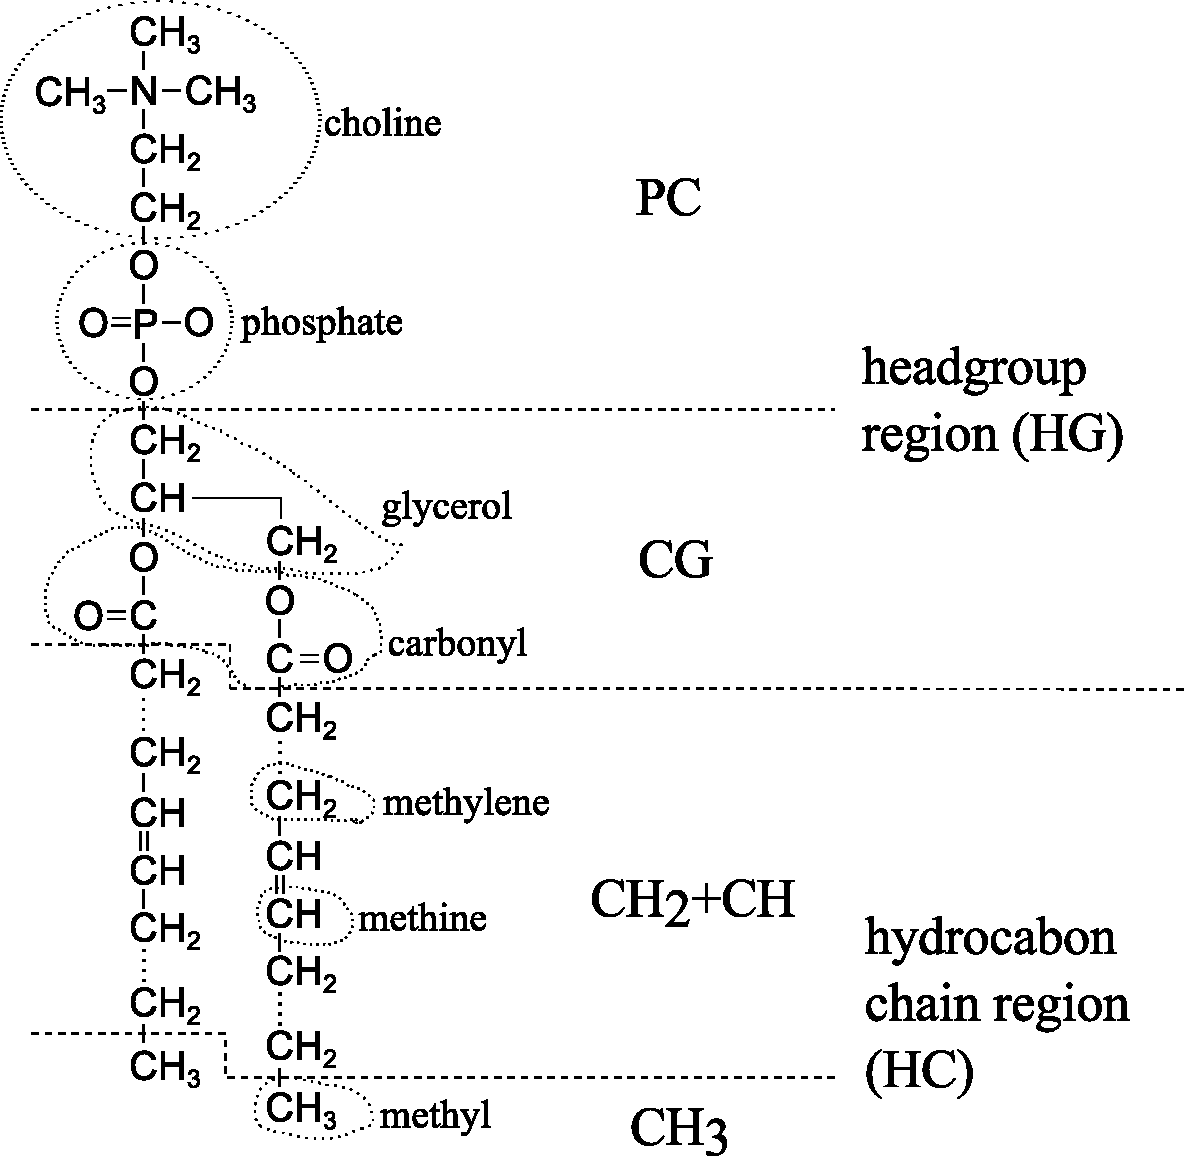
\includegraphics[scale=0.7]{./figures/Tat/dopc_schematic.pdf}
  \caption{Schematic of DOPC showing each lipid component. The dash lines 
           show where the lipid is divided into different components. 
           The lipid headgroup
           is divided into two components, phophate-choline and carbonyl-glycerol. 
           The hydrocarbon chain region is also divided
           into two components, methelence+methine and terminal methyl groups.}
  \label{fig:dopc_schematic}
\end{figure}
%------------------------------------------------------------------------------

%%%%%%%%%%%%%%%%%%%%%%%%%%%%%%%%%%%%%%%%%%%%%%%%%%%%%%%%%%%%%%%%%%%%%%%%%%%%%%%
\subsubsection{Functional forms}
Our model for electron density profile (EDP)
of Tat/lipid bilayer system consists of five structural subgroups: PC, CG,
CH$_2$+CH, CH$_3$, and Tat. 
(Fig.~\ref{fig:DOPC_EDP1}).
\begin{figure}[htbp]
  \centering
  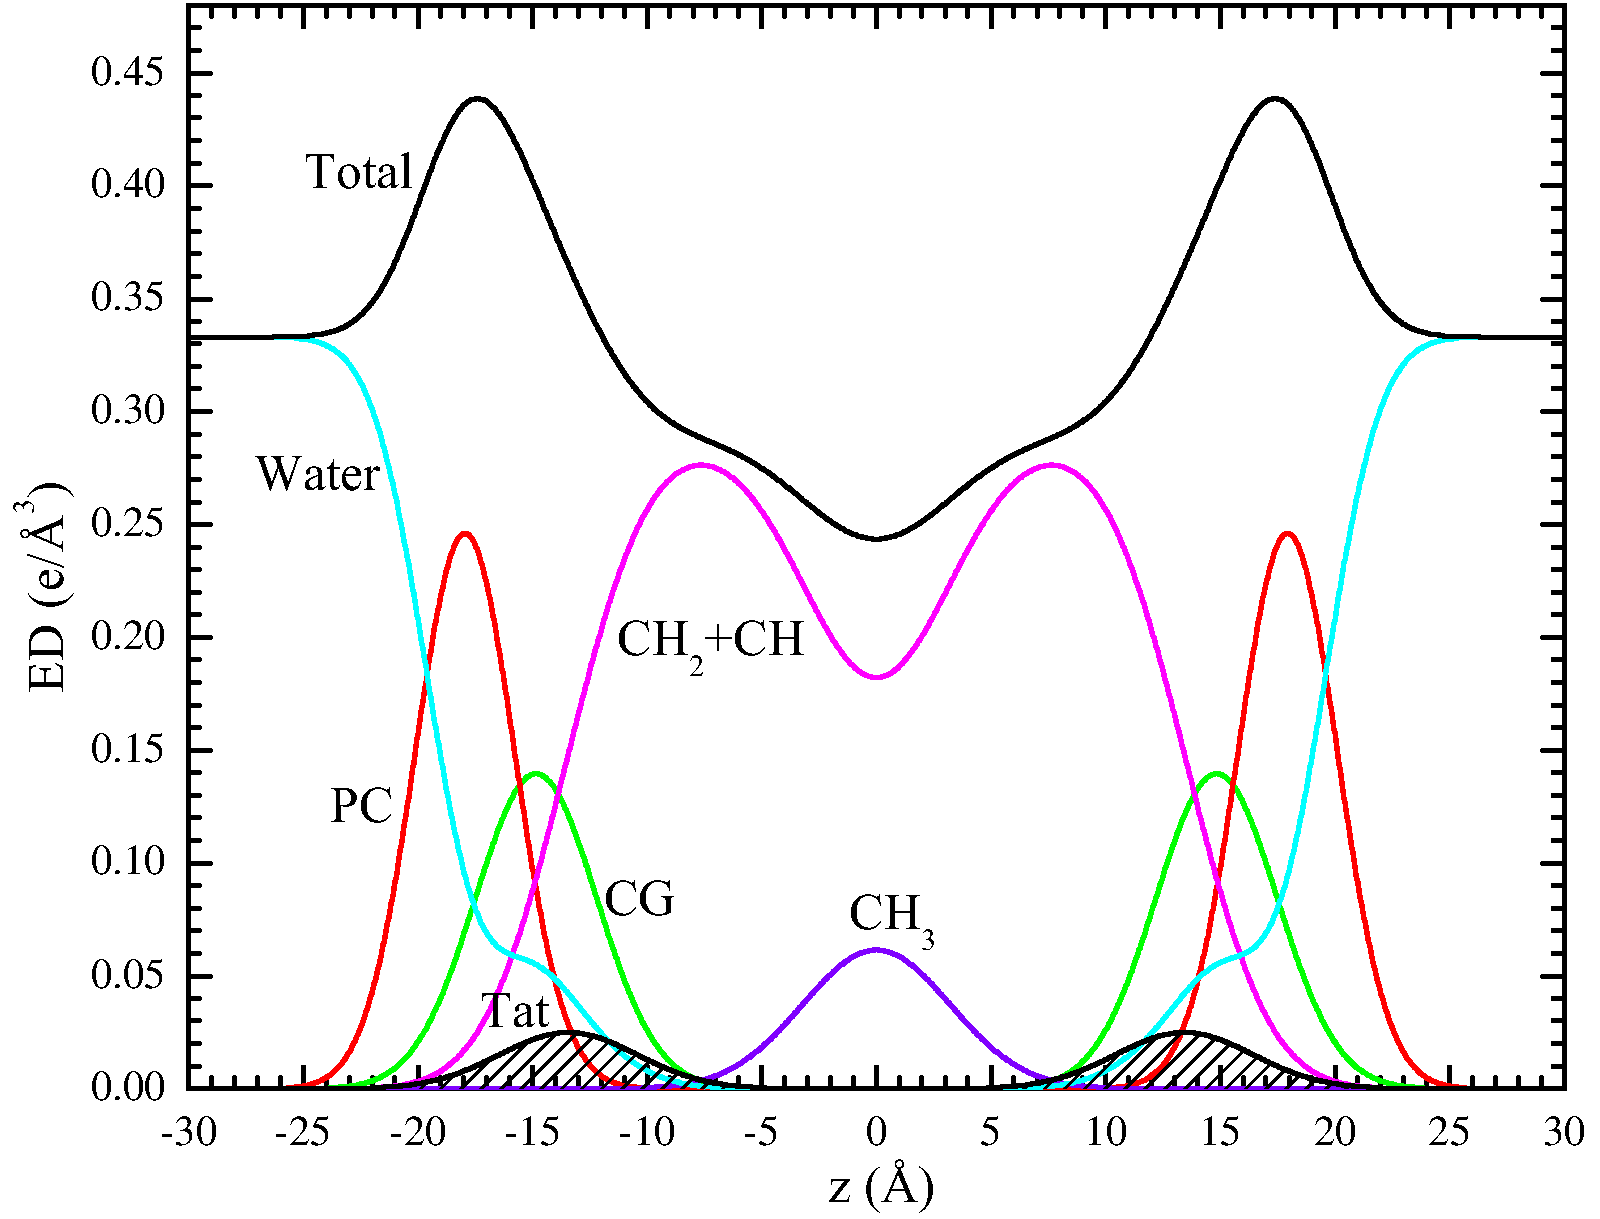
\includegraphics[width=\textwidth]{figures/Tat/SDP_Results/EDP/DOPC_Tat_model_EDP}
  \caption{A model electron density profile for DOPC with Tat.}
  \label{fig:DOPC_EDP}
\end{figure}
The volume probability distributions of components PC, CG, CH$_3$, and Tat 
are described by Gaussian functions,
\begin{equation}
  P_i(z)=\frac{c_i}{\sqrt{2\pi}}\pars{
    \exp\braces{-\frac{(z+z_i)^2}{2\sigma_i^2}}
	+ \exp\braces{-\frac{z-z_i)^2}{2\sigma_i^2}}
  },
\end{equation}
where $c_i$ is an integrated area underneath the curve and the two parts of the 
expression describe the two bilayer leaflets. 

The hydrocarbon chain region (HC) is represented by error functions,
\begin{equation}
  \PHC(z) = \frac{1}{2}\bracks{
    \mathrm{erf}(z,-\z{HC},\sigmaHC) - \mathrm{erf}(z,\z{HC},\sigmaHC)
  },
\end{equation}
where
\begin{equation}
  \mathrm{erf}(z,z_i,\sigma_i)=\frac{2}{\sqrt{\pi}}
    \int_0^{\frac{z-z_i}{\sqrt{2\sigma}}} \dx e^{-x^2}.
\end{equation}
The volume probability distribution for the methylene and methine group
combination can then be expressed as
\begin{equation}
  \PCHtwoCH(z) = \PHC(z)-\PCHthree(z).
  \label{eq:modelA}
\end{equation}
This definition enforces the total probability $\PHC$ in the hydrocarbon
chain region to equal one, which in turn means that placement of Tat in the  
chain region is prohibited. We call the model defined by Eq.~(\ref{eq:modelA})
model A (better name?). To allow Tat to be placed inside the hydrocarbon
chain region, we also consider an alternative definition,
\begin{equation}
  \PCHtwoCH(z) = \PHC(z)-\PCHthree(z) - \PTat(z),
\end{equation}
where the volume probability of CH$_2$+CH combined component is reduced by 
the Tat volume probability distribution. We call this model B.
The spatial conservation requires the water volume probability distribution 
to be
\begin{equation}
  \PW(z) = 1-\PPC(z)-\PCG(z)-\PTat(z)-\PHC(z)
\end{equation}
for model A and
\begin{equation}
  \PW(z) = 1-\PPC(z)-\PCG(z)-\PHC(z)
\end{equation}
for model B. 

Because X-rays measure the contrast between the bilayer and surrounding solvents, 
water, the experimental form factor is compared to the water subtracted model
form factor,
\begin{equation}
  F(q_z) = 2\int_0^{\frac{D}{2}} \dz \pars{
    \sum_i(\rho_i-\rhoW)P_i(z)
  } \cos(q_zz),
\end{equation}
where $i$ = PC, CG, Tat, CH+CH$_2$, and CH$_3$.

%%%%%%%%%%%%%%%%%%%%%%%%%%%%%%%%%%%%%%%%%%%%%%%%%%%%%%%%%%%%%%%%%%%%%%%%%%%%%%%
\subsubsection{Constraints}
The height of the hydrocarbon chain error function is fixed to one by imposing
spatial conservation, whereas the mean position of the terminal methyls is
fixed to $\zCHthree=0$ by symmetry arguments. The total lipid volume
$\VL$ is fixed to the experimentally measured value. 
The headgroup volume $\VHL$ was determined to be 331 \AA$^3$ for 
gel phase phosphatidylcholine bilayers \cite{ref:Tristram-Nagle02},
and we assume the same volume for the fluid phase phosphatidylcholine bilayers.
The volumes of PC and CG components satisfy
\begin{equation}
  \VPC + \VCG = \VHL,
\end{equation}
and the volumes of CH$_3$ and CH$_2$+CH components satisfy
\begin{equation}
  2\left(16\VCHtwoCH + \VCHthree\right) = \VL-\VHL.
\end{equation}
These component volumes constrain the height of the Gaussians as
\begin{align}
  \cPC &= \frac{\VPC}{\AL\sigmaPC} \\
  \cCG &= \frac{\VCG}{\AL\sigmaCG} \\
  \cCHthree &= \frac{2\VCHthree}{\AL\sigmaCHthree} \\
  \cTat &= \frac{\VTat}{\AL\sigmaTat}
\end{align}
where $\AL$ is area per lipid.

The ratio of 
the carbonyl/glycerol volume to the headgroup volume $\VHL$ was
reported to be 0.41 \cite{ref:Braun13}, so we constrain the CG
component volume to 135.7 \AA$^3$ and the PC component volume to 
195.3 \AA$^3$. 

The most detailed structural study on DOPC to date was published 
by Braun \textit{et al.} \cite{ref:Braun13}, 
and many of constraints on our model parameters can be derived
from their study. However, in that work, the authors used the 
SDP model \cite{ref:Kucerka08}, which is specifically tailored for
combined analysis of neutron and X-ray form factors. 
Therefore, we need to convert their structural results to the 
corresponding parameters in our simpler model. For example, 
from the reported values of the ratio of the volumes of the chain terminal
methyl (CH$_3$) to the chain methylenes (CH$_2$) and the ratio of 
the volumes of the chain methines (CH) to the chain methylenes, we can
calculate the ratio $\rCHthree$ of the volumes of CH$_3$ to the CH$_2$ and
CH combined component.  
Furthermore, the study by Braun \textit{et al.} was at 30 \textcelsius\
while our study was at 37 \textcelsius, so our
measured volume of DOPC was slightly higher.

At 30 \textcelsius, the volume of DOPC was reported to be 1303 \AA$^3$, 
so the volume of hydrocarbon chain region at the same temperature is 
$1303 - 331 = 972$ \AA$^3$. The ratio $r$ of the volumes
of the chain terminal methyl (CH$_3$) to the chain methylenes (CH$_2$) was 
reported to be 1.95, and the ratio $r_{12}$ of the volumes of the chain
methines (CH) to the chain methylenes 0.91 at 30 \textcelsius. 
Because there are 14 CH$_2$ groups,
2 CH groups, and 1 CH$_3$ group in each DOPC hydrocarbon chain, we have
$2\times(14\VCHtwo+2\VCH+\VCHthree)=972$ \AA$^3$. 
Using $\VCHthree/\VCHtwo=1.95$ 
and $\VCH/\VCHtwo=0.91$, we get $\VCHtwo=27.3$ \AA$^3$, 
$\VCH=24.9$ \AA$^3$, and $\VCHthree=53.3$ \AA$^3$. 
These calculated volumes lead to $\VCHthree/\VCHtwoCH=1.97$  for 30 \textcelsius. 

At 37 \textcelsius, the volume of DOPC was measured to be 1313.5 \AA$^3$, so
we have $2\times(16\VCHtwoCH+\VCHthree)=1313.5-331$. Assuming that the ratio 
$\VCHthree/\VCHtwoCH$ at 37 \textcelsius\ is the same as that at 30 \textcelsius\ 
gives $\VCHtwoCH=27.3$ \AA$^3$ and $\VCHthree=53.9$ \AA$^3$. We constrain
the components for the hydrocarbon chain region in our model 
to these calculated values.
%------------------------------------------------------------------------------
\begin{table}[htbp]
  \centering
  \begin{tabular}{ cc }
  \hline
    number of e/lipid & 434 \\ 
    volume/lipid (\AA$^3$) & 1313.5 \\
  \hline
  \end{tabular}
  \quad
  \begin{tabular}{ cccc }
    \hline
    component & $n^e_i$ & $V_i$ (\AA$^3$) & $\rho_i$ (e/\AA$^3$) \\
    \hline 
    PC & 97 & 195.3 & 0.497 \\  
    CG & 67 & 135.7 & 0.494 \\  
    CH$_2$+CH & 7.875 & 27.3 & 0.288 \\
    CH$_3$ & 9 & 53.9 & 0.167 \\
    \hline
  \end{tabular}
  \caption{DOPC basic structural parameters. $n^e_i$ and $\rho_i$ are
  the number of electrons and average electron density per component, 
  respectively.}
  \label{tb:DOPC_basic_params}
\end{table}
%------------------------------------------------------------------------------
\begin{table}[htbp]
  \centering
  \begin{tabular}{ cc }
  \hline
    number of e/lipid & 410 \\ 
    volume/lipid (\AA$^3$) & 1212.3 \\
  \hline
  \end{tabular}
  \quad
  \begin{tabular}{ cccc }
    \hline
    component & $n^e_i$ & $V_i$ (\AA$^3$) & $\rho_i$ (e/\AA$^3$) \\
    \hline 
    PE & 73 & 94.1 & 0.776 \\  
    CG & 67 & 135.7 & 0.494 \\  
    CH$_2$+CH & 7.875 & 27.3 & 0.288 \\
    CH$_3$ & 9 & 53.9 & 0.167 \\
    \hline
  \end{tabular}
  \caption{DOPE basic structural parameters. The notations are the same
  as in Table~\ref{tb:DOPC_basic_params}.}
  \label{tb:DOPE_basic_params}
\end{table}
%------------------------------------------------------------------------------
\begin{table}[htbp]
  \centering
  \begin{tabular}{ cc }
  \hline
    number of e/lipid & 428 \\ 
    volume/lipid (\AA$^3$) & 1288.2 \\
  \hline
  \end{tabular}
  \quad
  \begin{tabular}{ cccc }
    \hline
    component & $n^e_i$ & $V_i$ (\AA$^3$) & $\rho_i$ (e/\AA$^3$) \\
    \hline 
    PC/PE & 91 & 170 & 0.535 \\  
    CG & 67 & 135.7 & 0.494 \\  
    CH$_2$+CH & 7.875 & 27.3 & 0.288 \\
    CH$_3$ & 9 & 53.9 & 0.167 \\
    \hline
  \end{tabular}
  \caption{DOPC:DOPE (3:1) basic structural parameters. The notations are the same
  as in Table~\ref{tb:DOPC_basic_params}.}
  \label{tb:PCPE3:1_basic_params}
\end{table}
%------------------------------------------------------------------------------
\begin{table}[htbp]
  \centering
  \begin{tabular}{ ccc }
    \hline
    number of e/Tat & 838 \\ 
    volume/Tat (\AA$^3$) & 1877 \\
    $\rho_\textrm{Tat}$ (e/\AA$^3$) & 0.446 \\
    \hline
  \end{tabular}
  \quad
  \begin{tabular}{ ccc }
    \hline
    ratio & $n^e_\textrm{Tat}$ & $\VTat$ (\AA$^3$) \\    
    \hline
    62:1 & 13.6 & 30.5 \\
    28:1 & 29.5 & 66.1 \\
    16:1 & 53.0 & 118.8 \\
    \hline
  \end{tabular}
  \caption{Tat basic structural parameters. The notations are the same
  as in Table~\ref{tb:DOPC_basic_params}.}
  \label{tb:Tat_basic_params}
\end{table}
%------------------------------------------------------------------------------
\begin{table}[htbp]
  \centering
  \begin{tabular}{ |c|c|c|c|c|c|c|c| }
    \hline
     & DOPC & \multicolumn{2}{c|}{62:1} & \multicolumn{2}{c|}{28:1} & \multicolumn{2}{c|}{16:1} \\
    \cline{3-8}
     & & A & B & A & B & A & B \\
    \hline
    $\VL$ & 1314 & 1344 & 1344 & 1380 & 1380 & 1432 & 1432 \\    
    $\VHL$ & 331 & 362 & 331 & 397 & 331 & 450 & 331 \\  
    $\VTat$ & 0 & 30.5 & 30.5 & 66.1 & 66.1 & 119 & 119 \\  
    $\RPC$ & 0.59 & 0.54 & 0.59 & 0.49 & 0.59 & 0.43 & 0.59 \\
    $\RCG$ & 0.41 & 0.38 & 0.41 & 0.34 & 0.41 & 0.30 & 0.41 \\
    $\RTat$ & 0   & 0.08 & 0    & 0.17 & 0    & 0.27 & 0 \\ 
    $r_{12}$ & 0 & 0 & 0.558 & 0 & 1.21 & 0 & 2.17 \\
    $r$ & 1.97 & 1.97 & 1.97 & 1.97 & 1.97 & 1.97 & 1.97 \\ 
    \hline
  \end{tabular}
  \caption{Volumetric constraints. A and B refer to two different models 
  described in the text.}
  \label{tb:model_constraints}
\end{table}
%------------------------------------------------------------------------------

%%%%%%%%%%%%%%%%%%%%%%%%%%%%%%%%%%%%%%%%%%%%%%%%%%%%%%%%%%%%%%%%%%%%%%%%%%%%%%%
\subsection{Molecular Dynamics Simulation}
This section describes the MD simulations performed by Dr. Kun Huang.
Systems with different DOPC/Tat mole ratios (128:0, 128:2 and 128:4, corresponding to
0, 0.015 and 0.030 mole fractions) were simulated atomistically using the Gromacs 4.6.1
package \cite{ref:Hess08}. 
DOPC was modeled by the Slipid force field 
\cite{ref:Jambeck12_JPCB,ref:Jambeck12_JCTC} 
and HIV Tat was modeled by Amber 99SB \cite{ref:Hornak06}. 
Tip3p water was used [53]. The number of Tats was divided equally on
each side of the bilayer to mimic experimental conditions. All systems were simulated at 310 K
with a constant area in the $x$-$y$ plane and 1 atm constant pressure in the $z$ direction. Each
system was simulated for 100 ns and the last 50 ns was used as the production run.
At each DOPC/Tat mole ratio, we studied systems with three different area/lipid ($\AL$).
For the DOPC system, we fixed $\AL$ = 68, 70, 72 \AA$^2$; 
DOPC/Tat (128:2), we fixed the $\AL$ = 72, 74, 76 \AA$^2$; 
DOPC/Tat (128:4), we fixed the $\AL$ = 72, 74, 76 \AA$^2$. 
For each DOPC/Tat system at fixed $\AL$, 
we then conducted seven independent simulations with the center of mass (COM) of
each Tat constrained at different bilayer depths from the bilayer center 
(18, 16, 14, 12, 10, 8 and 5 \AA). 
In total, 45 independent simulations were conducted. 
The goal of constrained simulations is to find the best match between 
experimental and MD simulation form factors. Comparison to
the X-ray form factors was performed using the SIMtoEXP software [54]. 
Additional details concerning the MD simulations are in Supplementary Data 6.

The center of mass (COM) distance between each peptide and the bilayer was 
constrained by an umbrella potential with a force constant $k$ of 3000 kJ/mol/nm$^2$. 
Essentially, this potential acts as a spring, 
where its potential energy depends on the deviation of the distance 
between the center of mass of Tat and DOPC from a prefered value, $z_0$,
\begin{equation*}
  U(z_1^{\textrm{Tat}},\ldots,z_1^{\textrm{DOPC}},\ldots) = 
  -\frac{1}{2} k 
  \pars{z_{\textrm{cm}}^{\textrm{Tat}} - z_{\textrm{cm}}^{\textrm{DOPC}} - z_0}^2.
\end{equation*}
Then, $-\partial U/\partial z_i$ is the external force acting 
on atom, $i$. Before applying this constraint, Tats were attached to 
the bilayer from the water region. During the first 20 ns for 
pre-equilibration, Tats were allowed to change their configuration,
which resulted in different configurations for each Tat when attached
to the bilayer. With this COM constraint, each Tat was allowed to move
laterally and rotate, changing its configuration during simulations.

%%%%%%%%%%%%%%%%%%%%%%%%%%%%%%%%%%%%%%%%%%%%%%%%%%%%%%%%%%%%%%%%%%%%%%%%%%%%%%%
\newpage
\section{Analysis of Molecular Dynamics Simulation Data}
\subsection{SIMtoEXP program}
This section briefly describes the SIMtoEXP program
developed by Dr. Norbert Kucerka \cite{ref:Kucerka10}. 

\subsection{Local Thinning of Membranes}
The SIMtoEXP program only gives the average quantities for each leaflet. 
While our x-ray data are sensitive to the bilayer avarage electron density,
local information of Tat-DOPC interactions can be obtained from MD simulations.
In this section, we discuss a method to extract a local membrane thickness
around the Tat peptides.

The presence of Tat may result in compression of lipid bilayer along 
$z$-direction. If so, the phosphorus-phosphorus distance $D_\textrm{PP}'$ 
of the bilayer near Tat may be different from the distance
$D_\textrm{PP}$ away from Tat.  
For small Tat concentration, $D_\textrm{PP}$ would be the same as that of 
pure DOPC if the 
distance from all Tats is large enough.  For our concentrations, 
the thinning effect may extend throughout the bilayer because the lateral
effect of Tat might have a larger lateral decay length than the distance 
between Tats. Whether that is the case or not, one would expect that the 
thickness near the Tats is smaller than the average thickness, and
$D_\textrm{PP}'$ is what we want to measure. 
%------------------------------------------------------------------------------
\begin{figure}[htbp]
  \centering
  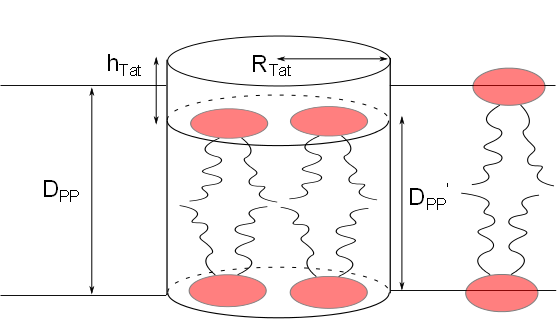
\includegraphics[scale=0.5]{./figures/Tat/cylinder_model}
  \caption{test}
  \label{fig:cylinder_model}
\end{figure}
%------------------------------------------------------------------------------
 
First, let us define what we mean by lipids close to Tat.  
As in Fig.~\ref{fig:cylinder_model}, we imagine a cylinder around Tat and 
pick up all the phosphorus atoms within it.  
Approximating Tat as a cylinder 
with its height given by the FWHM of its electron density distribution, 
its 
radius $R_\textrm{Tat}$ = 9 \AA comes from the volume of Tat = 1876 \AA$^3$ and 
$\hTat$ = 7.6 \AA
measured from one of the simulations. 
Let us define the lateral center of the 
cylinder in some way - a crude approximation would put it at the arginine in 
the middle of the amino acid sequence. Then let us define $D\textrm{PP}'$ 
using only 
those lipids whose phosphorus atoms lie within these 9 \AA cylinders around the 
Tats. Then $D_\textrm{PP} = \zphos^+ - \zphos^-$ where $\zphos^+$ and $\zphos^-$ 
are the 
average $Z$ of the n1 (n2) lipids in the upper and lower monolayer, respectively.  
To be more precise, assume that the arginine in the middle of the amino acid 
sequence is at the center of the cylinder. For a refined method, we could find 
the center of mass of each Tat and use them as the lateral center of cylinders 
(instead of a particular carbon atom in an arginine). 

The algorithm for doing this is straightforward.  For each time frame, 
the positions ($x_i$ ,$y_i$, $z_i$) of each Tat, $i$, are listed.   
We choose phosphorus atoms whose ($x$, $y$) lateral position lies within 
9 \AA of any one of the Tat's lateral position. Then, $z$ position
of the chosen phosphorus atoms are placed in a 
list. Then, $\zphos$ are calculated from the list. 
The number of selected phosphorus atoms in each monolayer was also 
recorded. This value gives local lateral depletion if the Tat cylinders 
are assumed not to overlap. We averaged over many snapshots to gain 
better statistics. 

\subsection{Lateral Decay Length of Membrane Thinning}
This section describes a method to measure the lateral decay length
of membrane thinning due to Tat-lipid interactions. 
As in the previous section, Tat is modeled here as a cylinder with 
its radius equal to $R_1$, height $\hTat$,
and volume $\VTat$ such that $R_1=\sqrt{\VTat/(\pi \hTat)}$. 
Let $h(r)$ represent the phosphorus height profile
of a leaflet. The two leaflets are assumed to be decoupled.
In our model, lipids are separated into three regions: 
suppressed, boundary, and unperturbed region . 
%------------------------------------------------------------------------------
\begin{figure}[htbp]
  \centering
  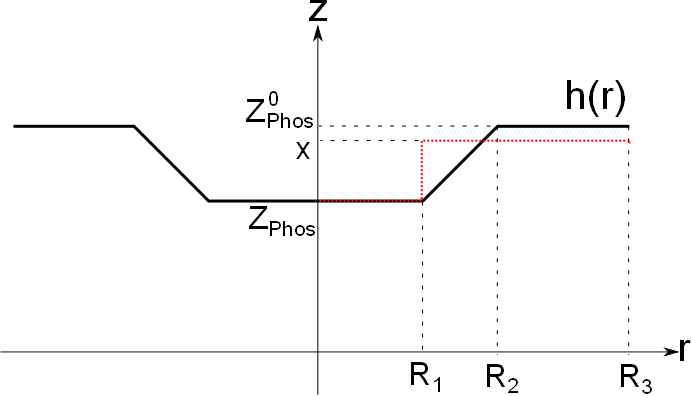
\includegraphics[scale=0.5]{./figures/Tat/linear_model.png}
  \caption{test}
  \label{fig:linear_model}
\end{figure}
%------------------------------------------------------------------------------
The suppressed region extends from $r=0$ to $R_1$ and is directly beneath 
(above) Tat in the top (bottom) leaflet. In this region, lipids are uniformly 
compressed by Tat toward the 
center of the bilayer, so that $h(r)$ is a constant equal to $\zphos$. 
From $r=R_1$ to $R_2$ is the boundary region, where $h(r)$ is assumed to 
linearly increase with the lateral distance $r$. The lateral decay length
of membrane thinning is given by $R_2-R_1$. 
In the unperturbed region ($r>R_3$), lipids do not interact with 
Tat, behaving identically to DOPC, so the phosphorus position is the same as that of 
DOPC. A continuous $h(r)$ that 
satisfies the above criteria is
\begin{equation}
  h(r) = \left\{ 
  \begin{array}{lcr}
    \zphos   & \text{if} & 0   \leq r < R_1 \\
    mr+b     & \text{if} & R_1 \leq r < R_2 \\
    \zphos^0 & \text{if} & R_2 \leq r < R_3 
  \end{array}\right.  
\end{equation}     
with $m=(\zphos-\zphos^0)/(R_1-R_2)$ and $b=(\zphos^0R_1-\zphos R_2)/(R_1-R_2)$. 
Assuming that the simulation box is a cylinder gives 
$R_3=\sqrt{N\AL/\pi}$. 
$\zphos$ can be measured directly from simulation trajectories.
$\zphos^0$ is a half of the average phosphorus-phosphorus distance 
in a DOPC simulation,
which can be easily obtained from the SIMtoEXP program. 
The average height profile over
the monolayer, $\langle h(r) \rangle$, can be also obtained from the program 
in the same manner. 
The only unknown is $R_2$.

Let us calculate $\langle h(r) \rangle$. In the cylindrical coodinates, 
\begin{equation}
  \langle h(r) \rangle 
  = \frac{1}{\pi R_3^2} \int_0^{2\pi}d\phi \int_0^{R_3}\dr rh(r)
\end{equation}
The $\phi$ integration is trivial. The $r$ integration is
\begin{align}
  & \int_0^{R_3}\dr rh(r) \nonumber\\
  &= \int_0^{R_1}\dr \zphos r + \int_{R_1}^{R_2}\dr (mr+b)r + \int_{R_2}^{R_3}\dr \zphos^0r \nonumber\\
  &= \frac{1}{2}\left[\zphos R_1^2+\zphos^0(R_3^2-R_2^2)\right] + 
     \frac{1}{3}m\left(R_2^3-R_1^3\right) + 
     \frac{1}{2}b\left(R_2^2-R_1^2\right) \nonumber\\        
  &= \frac{1}{2}\left[\zphos R_1^2+\zphos^0(R_3^2-R_2^2)\right] +
     \frac{1}{3}\left(\zphos^0-\zphos\right)\left(R_2^2+R_1R_2+R_1^2\right) \nonumber\\
  &  + \frac{1}{2}\left(\zphos R_2-\zphos^0 R_1\right)\left(R_1+R_2\right) \label{eq:r_integ}
\end{align}
Using Eq.~(\ref{eq:r_integ}), we get 
\begin{equation}
  \langle h(r) \rangle 
  = \frac{\left(\zphos-\zphos^0\right)\left(R_1^2+R_1R_2+R_2^2\right)+3\zphos^0R_3^2}{3R_3^2}
  \label{eq:quadR2}
\end{equation}
Eq.~\ref{eq:quadR2} is a quadratic equation in terms of $R_2$. 
Solving for $R_2$ gives
\begin{equation}
  R_2 = \frac{-R_1+\sqrt{R_1^2+4C}}{2} 
\end{equation}
with
\begin{equation}
  C = \frac{3R_3^2\left(\zphos^0-\langle h(r)\rangle\right)}{\zphos^0-\zphos} - R_1^2
\end{equation}

%%%%%%%%%%%%%%%%%%%%%%%%%%%%%%%%%%%%%%%%%%%%%%%%%%%%%%%%%%%%%%%%%%%%%%%%%%%%%%%
\section{Results}
\subsection{Bending and Bulk Modulus}\label{sec:Kc_results}
Show X-ray data. Show fitting boxes.
Show the Kc values.
Also, show the resultant
form factors, which qualitatively show the membrane thinning.
Fig. XX shows the scattering intensity pattern from DOPC/DOPE (1:1) with mole 
fraction
x=0.034 Tat. The diffuse lobes are due to equilibrium fluctuations that occur 
in these fully
hydrated, oriented lipid/peptide samples. The intensity $I(q)$ in the diffuse 
patterns provide the
absolute values of the form factors $F(q_z)$, which are the Fourier transforms 
of the electron density
profile, through the relation $I(\mathbf{q})=S(\mathbf{q})|F(q_z)|2/q_z$, 
where $q=(q_r,q_z)$, $S(q)$ is 
the structure
interference factor, and $q_z^{−1}$ is the usual LAXS approximation to the 
Lorentz factor [39, 55, 56].
The first step in the analysis takes advantage of the $q_r$ dependence of the 
scattering to obtain the
bending modulus $K_C$ with results shown in Fig. 2. As positively charged Tat 
concentration was
increased, the lamellar repeat spacing $D$ generally increased in neutral lipid 
bilayers and
decreased in negatively charged bilayers, consistent with changes in 
electrostatic repulsive
interactions. With few exceptions, the water space between bilayers exceeded 
20 \AA.

The analysis that obtains $K_C$ also obtains the structure factor $S(\mathbf{q})$ 
and then the unsigned
form factors $|F(q_z)|$ are obtained from the intensity $I(q)$ by division. 
Results for five different
membrane mimics are shown in Fig. 3. Vertical lines indicate the “zero” position 
between the
lobes of diffuse data where $F(qz)$ change sign. In every sample, the zero 
positions shift to larger
$q_z$, indicating a thinning of the membranes.

%%%%%%%%%%%%%%%%%%%%%%%%%%%%%%%%%%%%%%%%%%%%%%%%%%%%%%%%%%%%%%%%%%%%%%%%%%%%%%%
\subsection{Volume results}\label{sec:volume_results}
(Should probably include this info in appendix)
First, the mass of Tat and water were measured to be 
3.7 and 1212.6 mg via a digital balance. The density of water and 
Tat-water solution were measured to be 0.993325 and 0.99418 $\mathrm{g/cm^3}$,
respectively. The measured values of these quantities
are shown in Table \ref{tb:values}.
%------------------------------------------------------------------------------
\begin{table}[ht]
  \centering
  \begin{tabular}{c c c}
    Molecule & Molecular Weight & Volume \\
    Tat (YGRKKRRQRRR) & 1560 & 1876 \\ 
    Tat + TFA & 2464 & 2964
  \end{tabular}
  \caption{Important Quantities for Tat Peptide}
  \label{tb:Tat}
\end{table}
%------------------------------------------------------------------------------
\begin{table}[ht]
  \centering
  \begin{tabular}{c c}
    $\rho_{sol}$ & 0.994180 $\mathrm{g/cm^3}$\\
    $\rho_w$ & 0.993325 $\mathrm{g/cm^3}$\\
    $m_w$ & 1212.6 mg \\
    $m_T$ & 3.73 mg \\ 
  \end{tabular}
  \caption{Measured Quantities in }
  \label{tb:values}
\end{table}
%------------------------------------------------------------------------------
This value is in a good agreement with the 
value calculated from a peptide calculator website \cite{}. 

Experimental and simulated volumes are given in Table 2. The simulated volume was
obtained using the volume app in the SIMtoEXP program. The experimental Tat volume was
calculated from the measured density assuming that the lipid volume was the same as with no
Tat. In general, there may be an interaction volume between the peptide and the lipid membrane
as we found previously for bacteriorhodopsin [57]. As lipid was present in excess to Tat, the
partial molecular volume of the lipid should be the same as with no Tat, so this way of
calculating includes all the interaction volume in VTat. Comparison of VTat in water with the
result for 5:1 Lipid:Tat suggests that the interaction volume may be negative, consistent with a
net attractive interaction with lipid. Understandably, values of VTat were unreliable for small
mole ratios of Tat:Lipid. Therefore we used simple additivity for those mimics not shown in
Table 2 for the volumes used in the SDP program. All volumes obtained from the Gromacs MD
simulations were somewhat smaller than the measured volumes, but it supports the Tat volume
being closer to 1822 Å3 than the outlying values obtained experimentally at small Tat
concentrations.

%%%%%%%%%%%%%%%%%%%%%%%%%%%%%%%%%%%%%%%%%%%%%%%%%%%%%%%%%%%%%%%%%%%%%%%%%%%%%%%
\subsection{Electron Density Profile Modeling}\label{sec:SDP_results}
Using the model described in section \ref{sec:SDP_method}, 
we fitted our measured X-ray form factors. In all fits,
the positions of component groups were free parameters, but we 
assumed that the lipid headgroup is somewhat rigid so that it cannot compress
or expand. This assumption led to fixing the distance
$\zPC-\zCG$ between the PC and CG components as well
as the distance $\zCG-\zHC$ between the CG component and the Gibbs dividing
surface for the hydrocarbon chains. 
We also constrained the width of Tat 
Gaussian. We fitted with three different values of widths,
2.5, 3.0, and 3.5, to study the range of variation due to the Tat width. 
The choice was made based on MD simulation results. (Check this again)
We constrained the Tat width 
because we found that this parameter tended to become very small
when it was free. This tendency to a unphysically small value was due to 
lack of higher $q_z$ data points. A very narrow feature in an electron density profile
led to large magnitude of the form factor at larger $q_z$. Because data 
points at larger $q_z$ were not available, this narrow feature did not get penalized. 
In wide angle X-ray scattering, which probes much larger $q_z$ than LAXS does,
we did not see much diffuse scattering for $q_z > 1.0$ \AA$^{-1}$ (data not shown).
Also, from a stereochemical point of view, a peptide width cannot be too small either.
These arguments allowed us to disregard the best fits with a too small value
of $\sigmaTat$.

Figure~\ref{fig:DOPC_Tat_XFF1} shows the results for DOPC with Tat. 
As shown, the fits were generally very good.  
Table~\ref{tb:DOPC_fit_results} shows the best fit parameters for DOPC bilayers.
It is clear that the area per lipid $\AL$ increased as the Tat concentration was
increased. An increase in $\AL$ implies thinning of the bilayer which is an 
incompressible membrane. The results for DOPC:DOPE (3:1) are shown in 
Fig.~\ref{fig:DOPCDOPE3to1_Tat_XFF1} and 
Table~\ref{tb:DOPCDOPE3to1_fit_results}, and the results for DOPC:DOPE (1:1) 
in Fig.~\ref{fig:DOPCDOPE1to1_Tat_XFF1} and 
Table~\ref{tb:DOPCDOPE1to1_fit_results}.
%------------------------------------------------------------------------------
\begin{figure}[htbp]
  \centering
  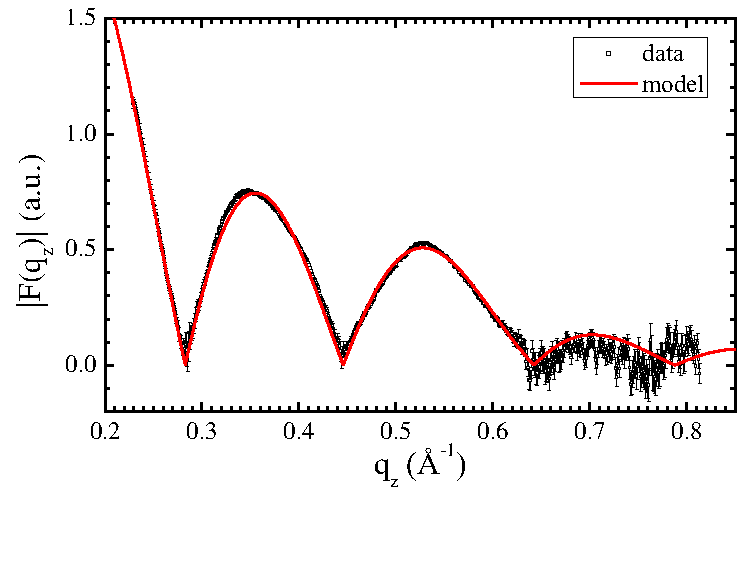
\includegraphics[width=0.45\textwidth,valign=t]{figures/Tat/SDP_Results/XFF/DOPC_XFF1} 
  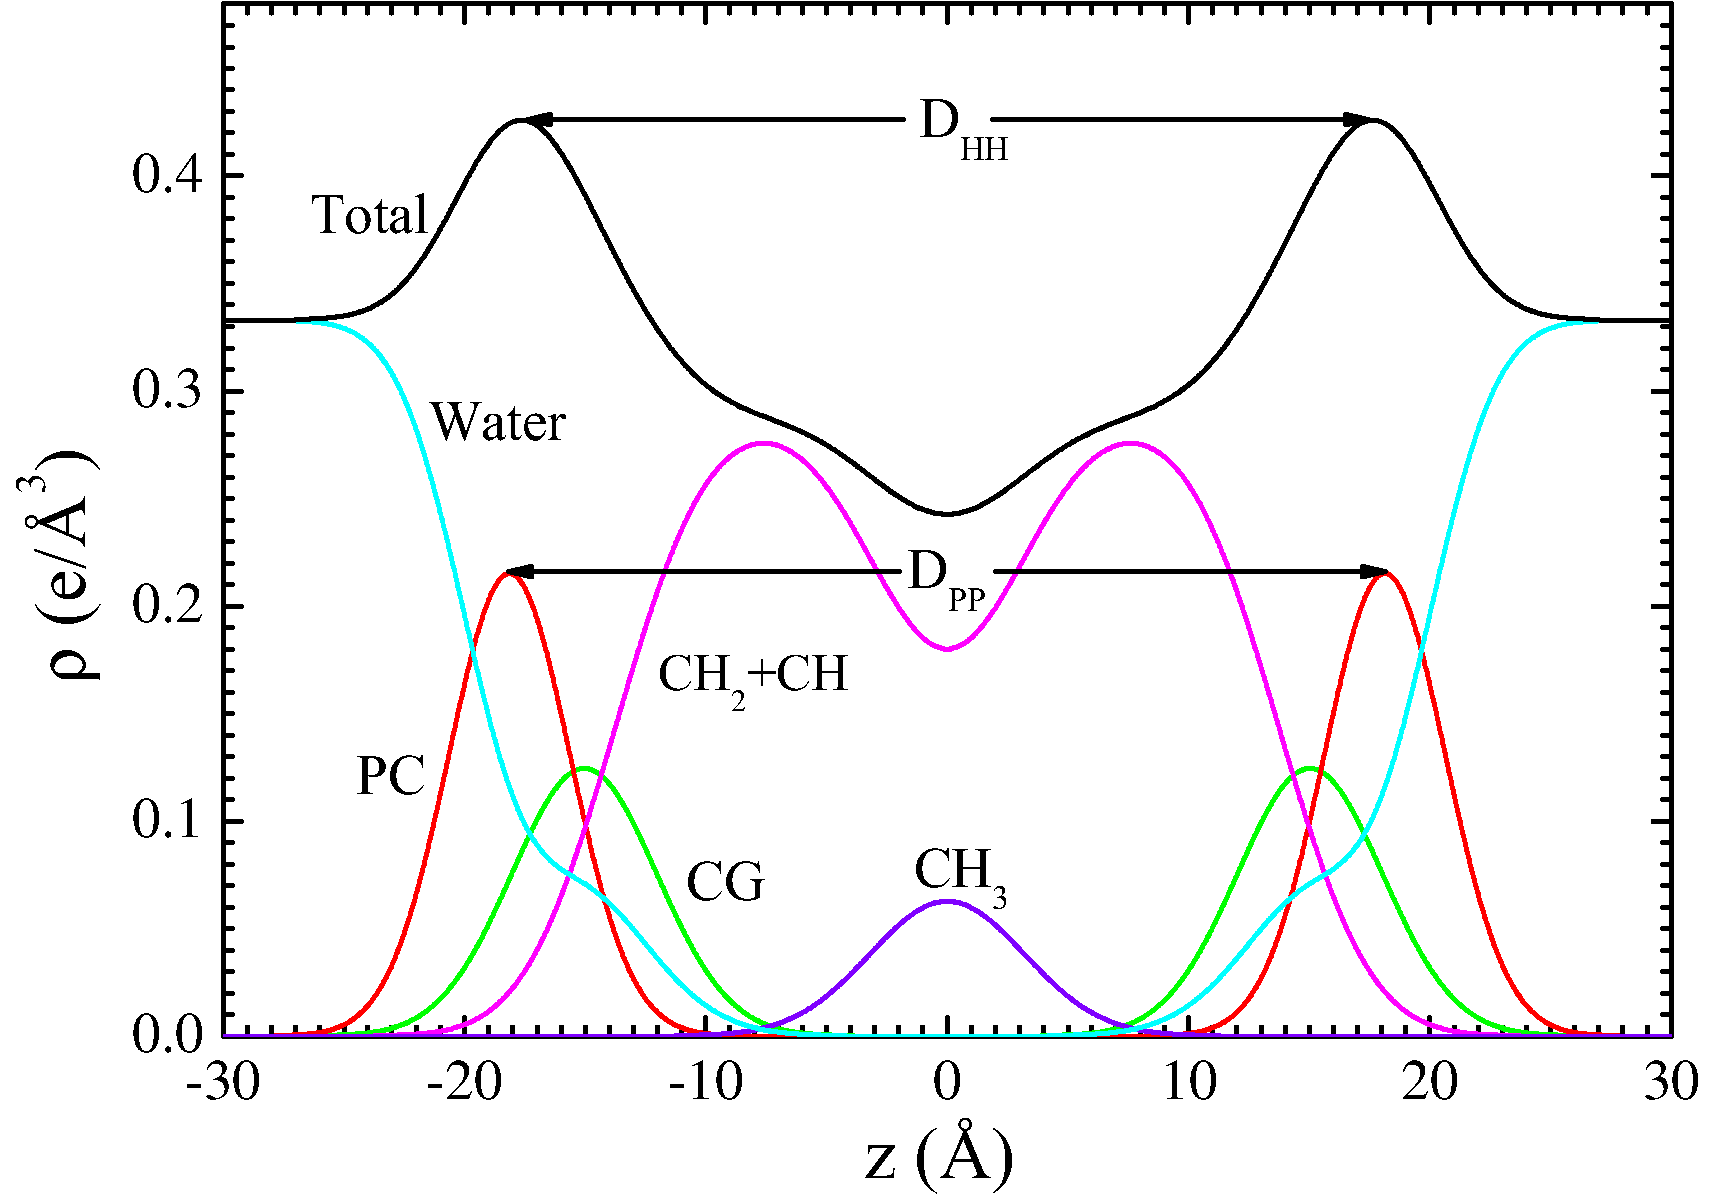
\includegraphics[width=0.45\textwidth,valign=t]{figures/Tat/SDP_Results/EDP/DOPC_EDP1} 
  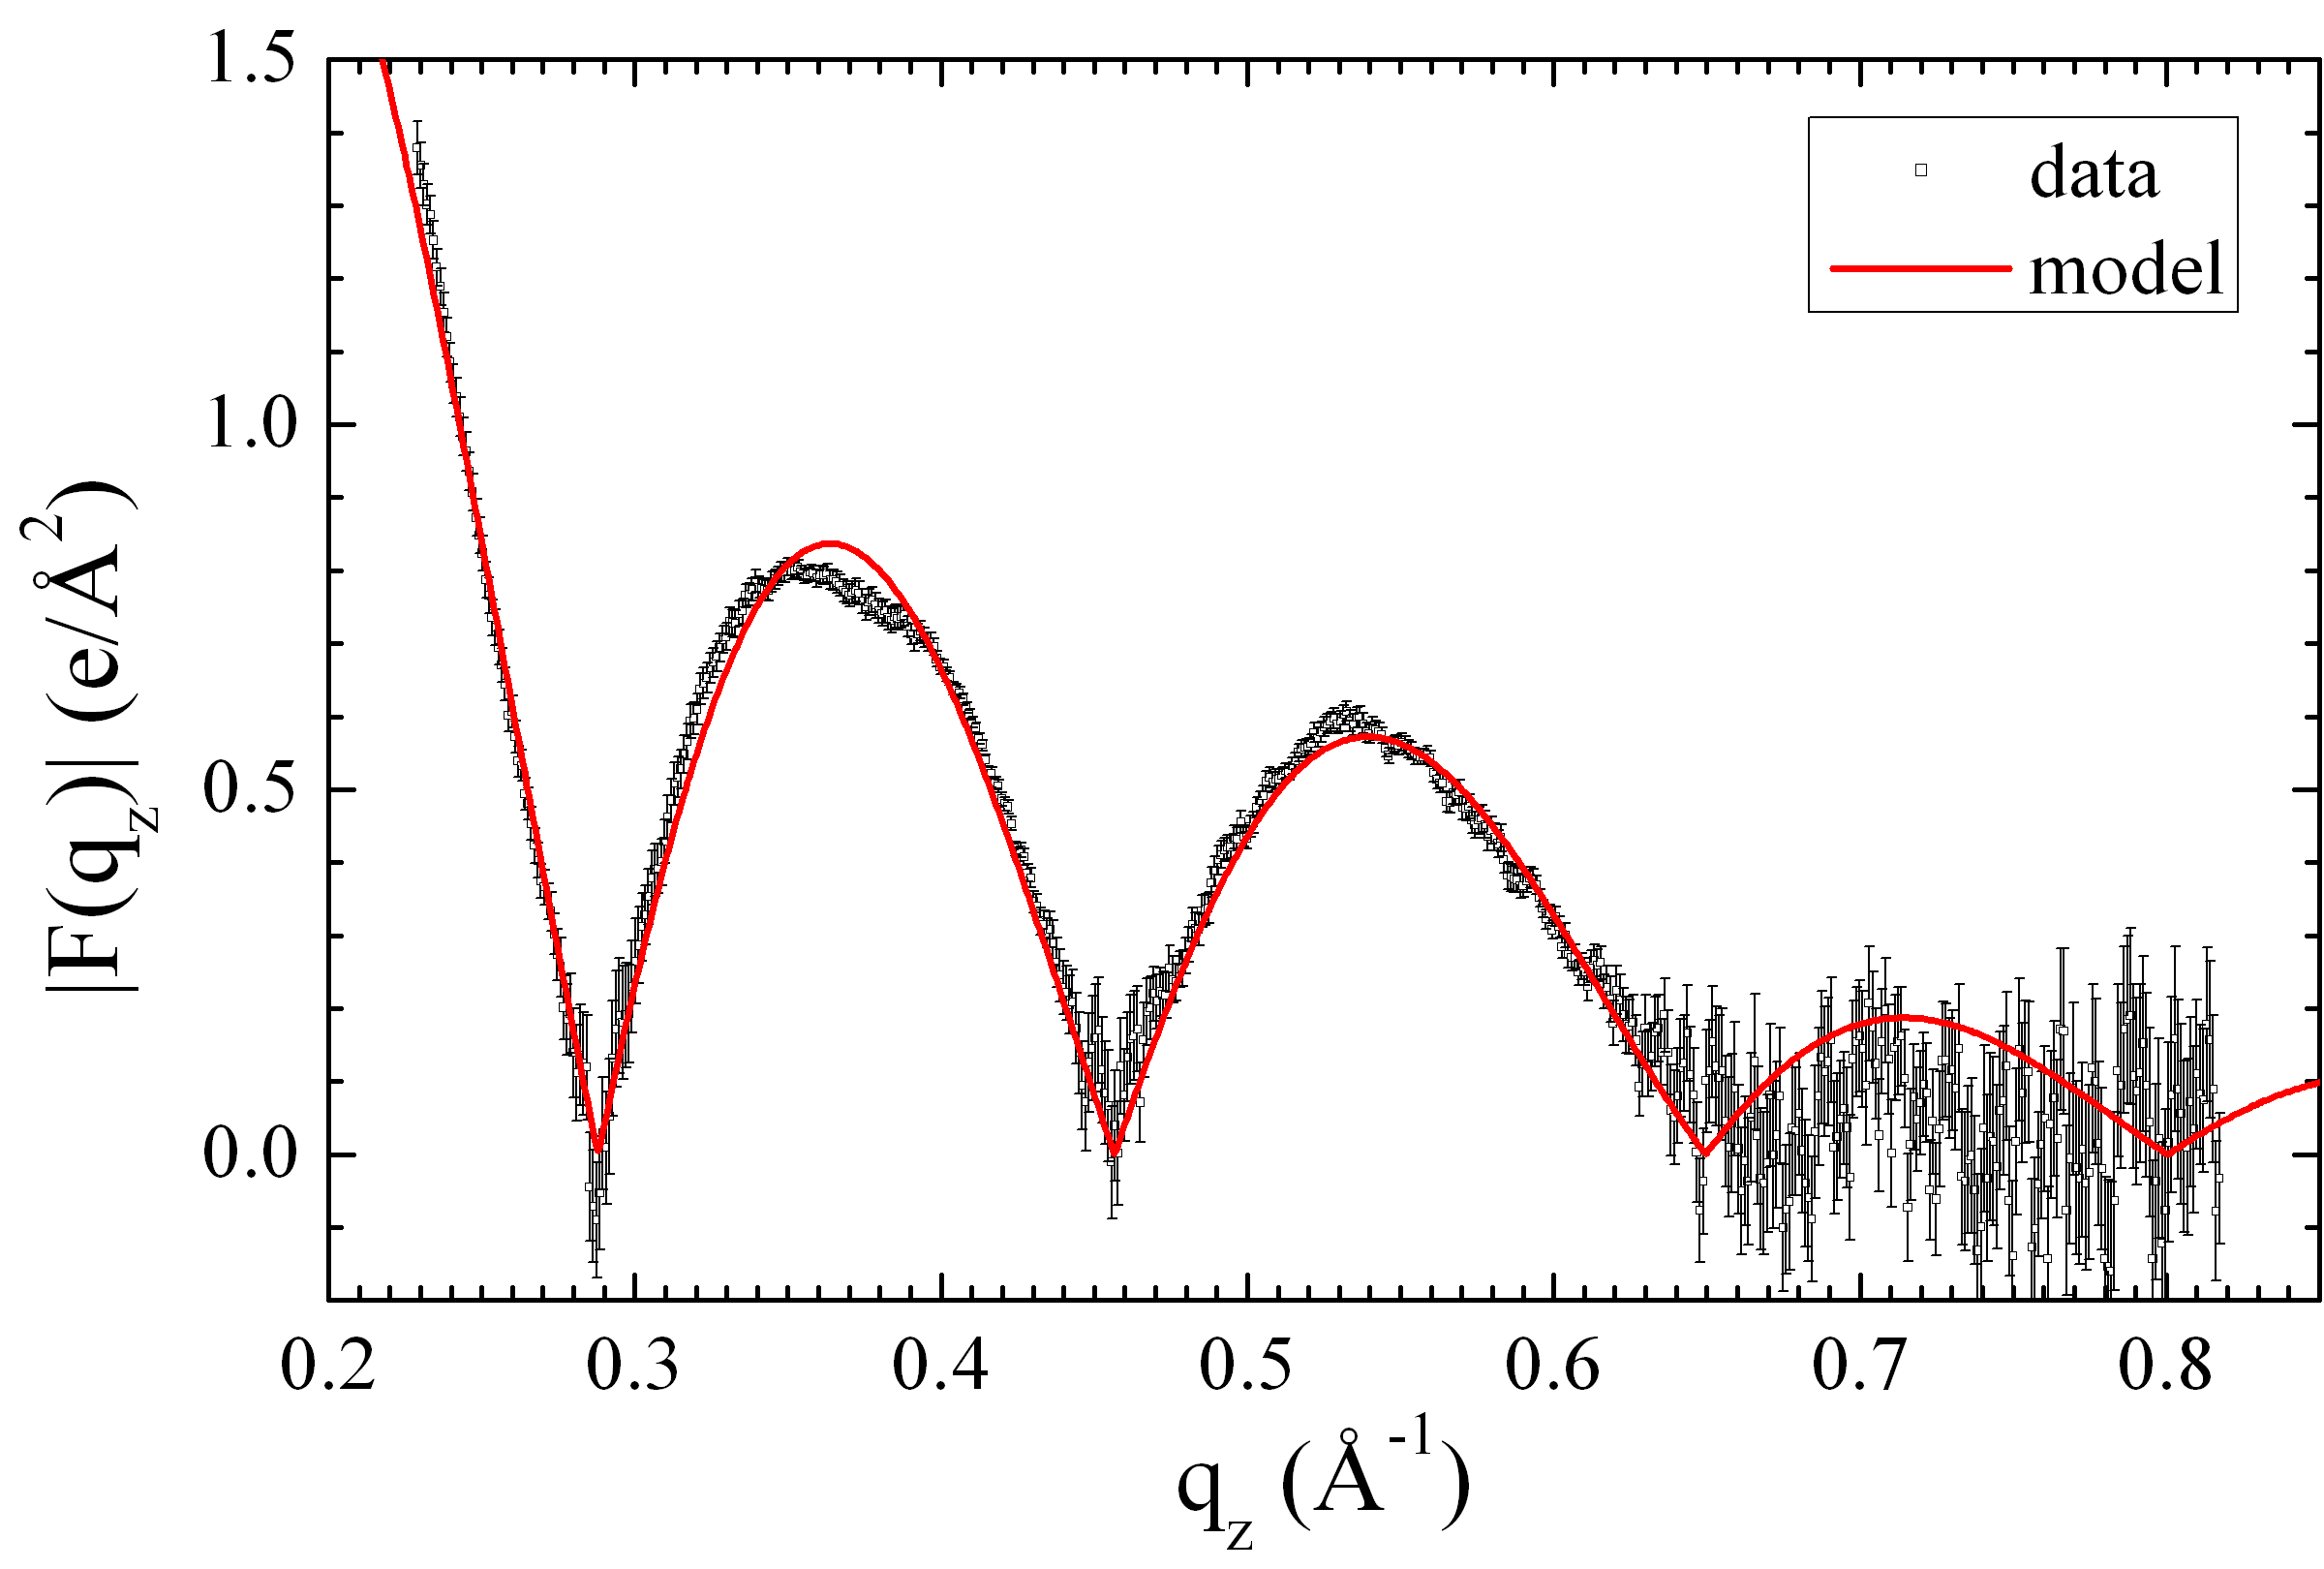
\includegraphics[width=0.45\textwidth,valign=t]{figures/Tat/SDP_Results/XFF/DOPC_Tat_62to1_3p0_XFF1}
  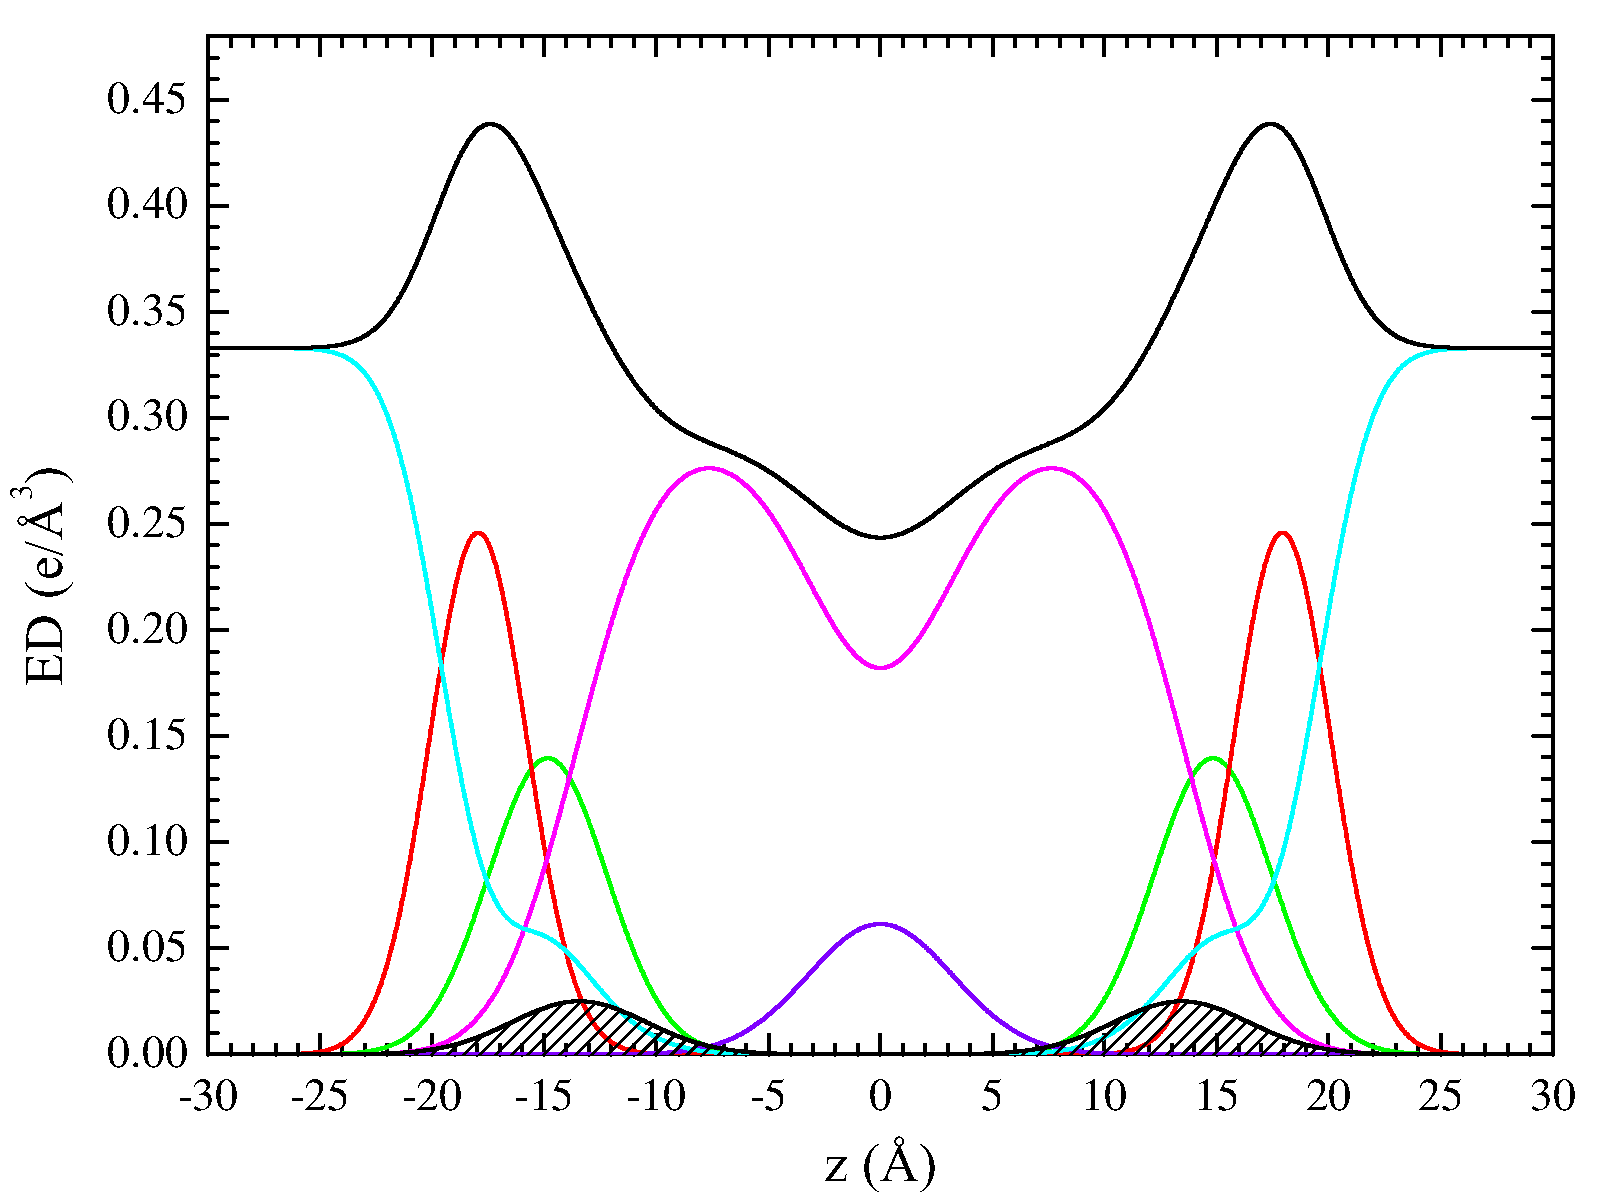
\includegraphics[width=0.45\textwidth,valign=t]{figures/Tat/SDP_Results/EDP/DOPC_Tat_62to1_3p0_EDP1} 
  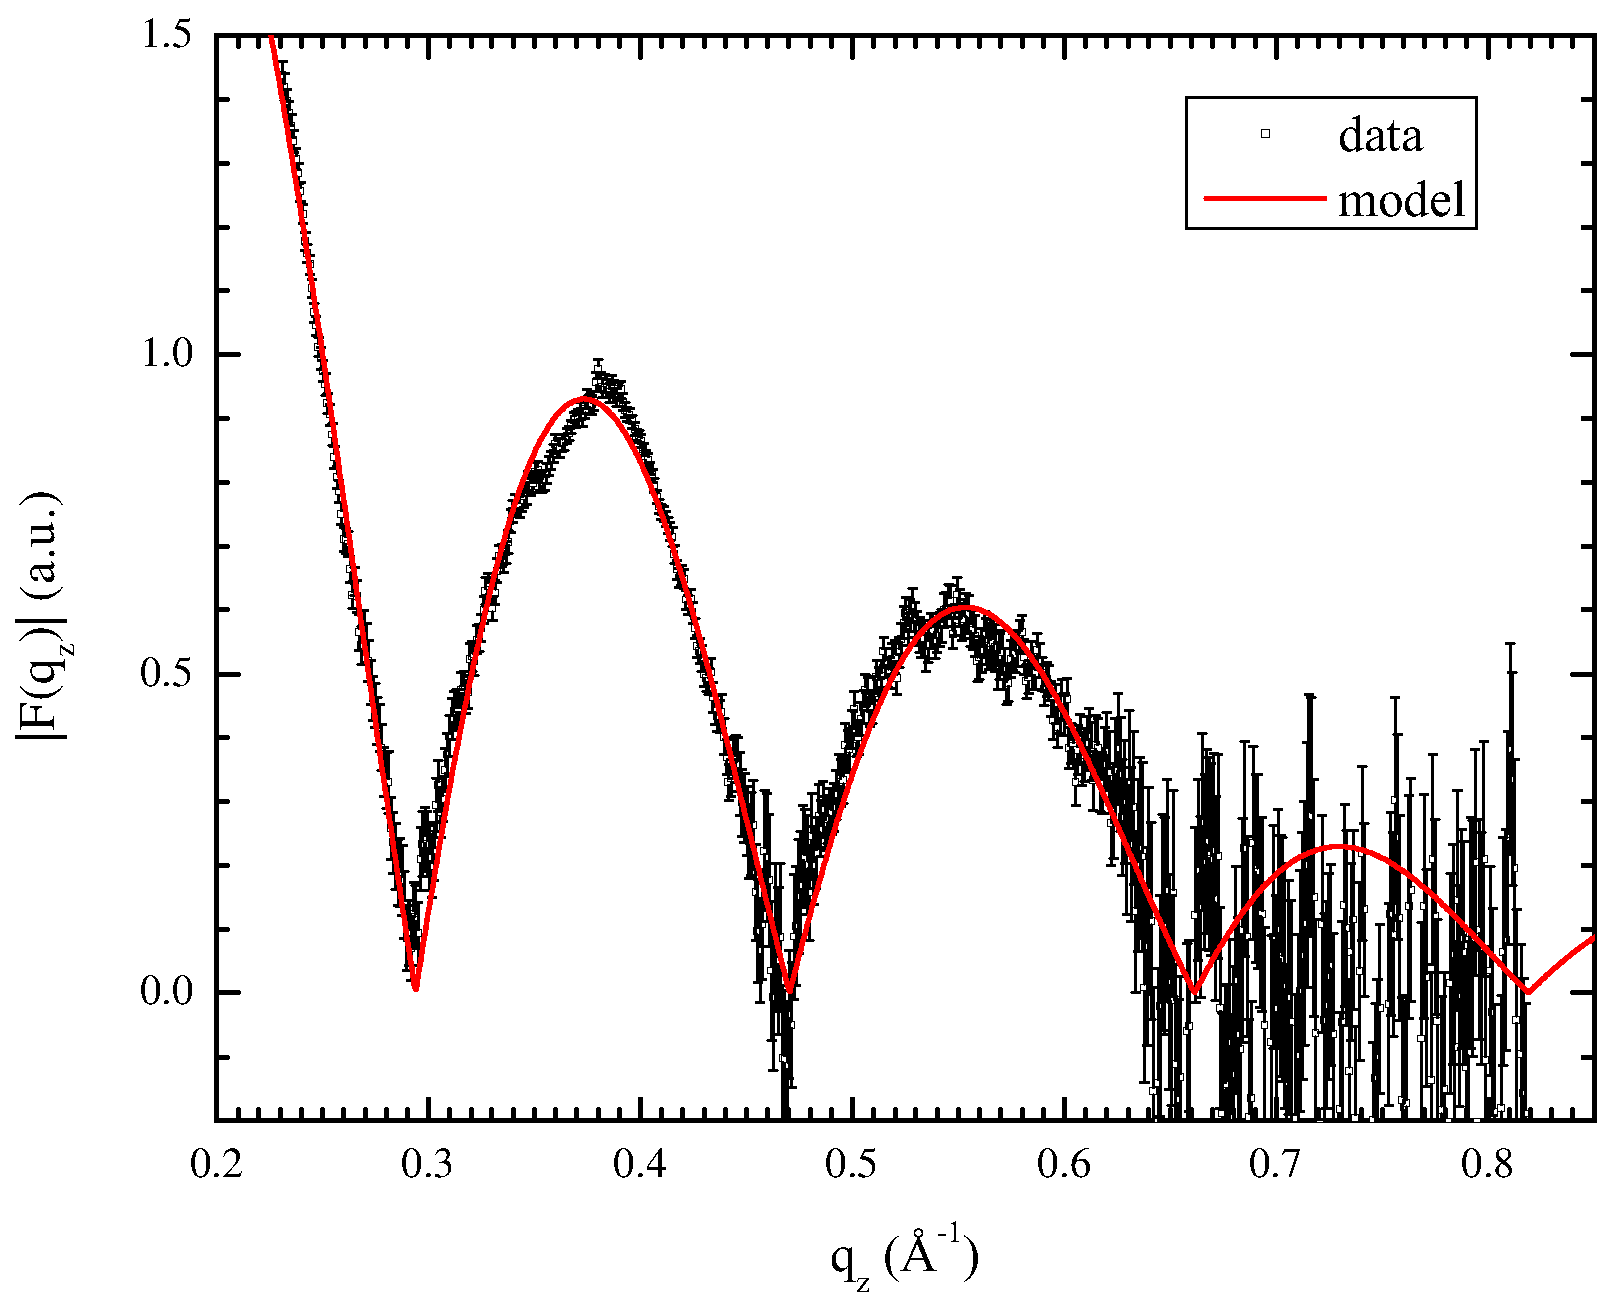
\includegraphics[width=0.45\textwidth,valign=t]{figures/Tat/SDP_Results/XFF/DOPC_Tat_28to1_3p0_XFF1}
  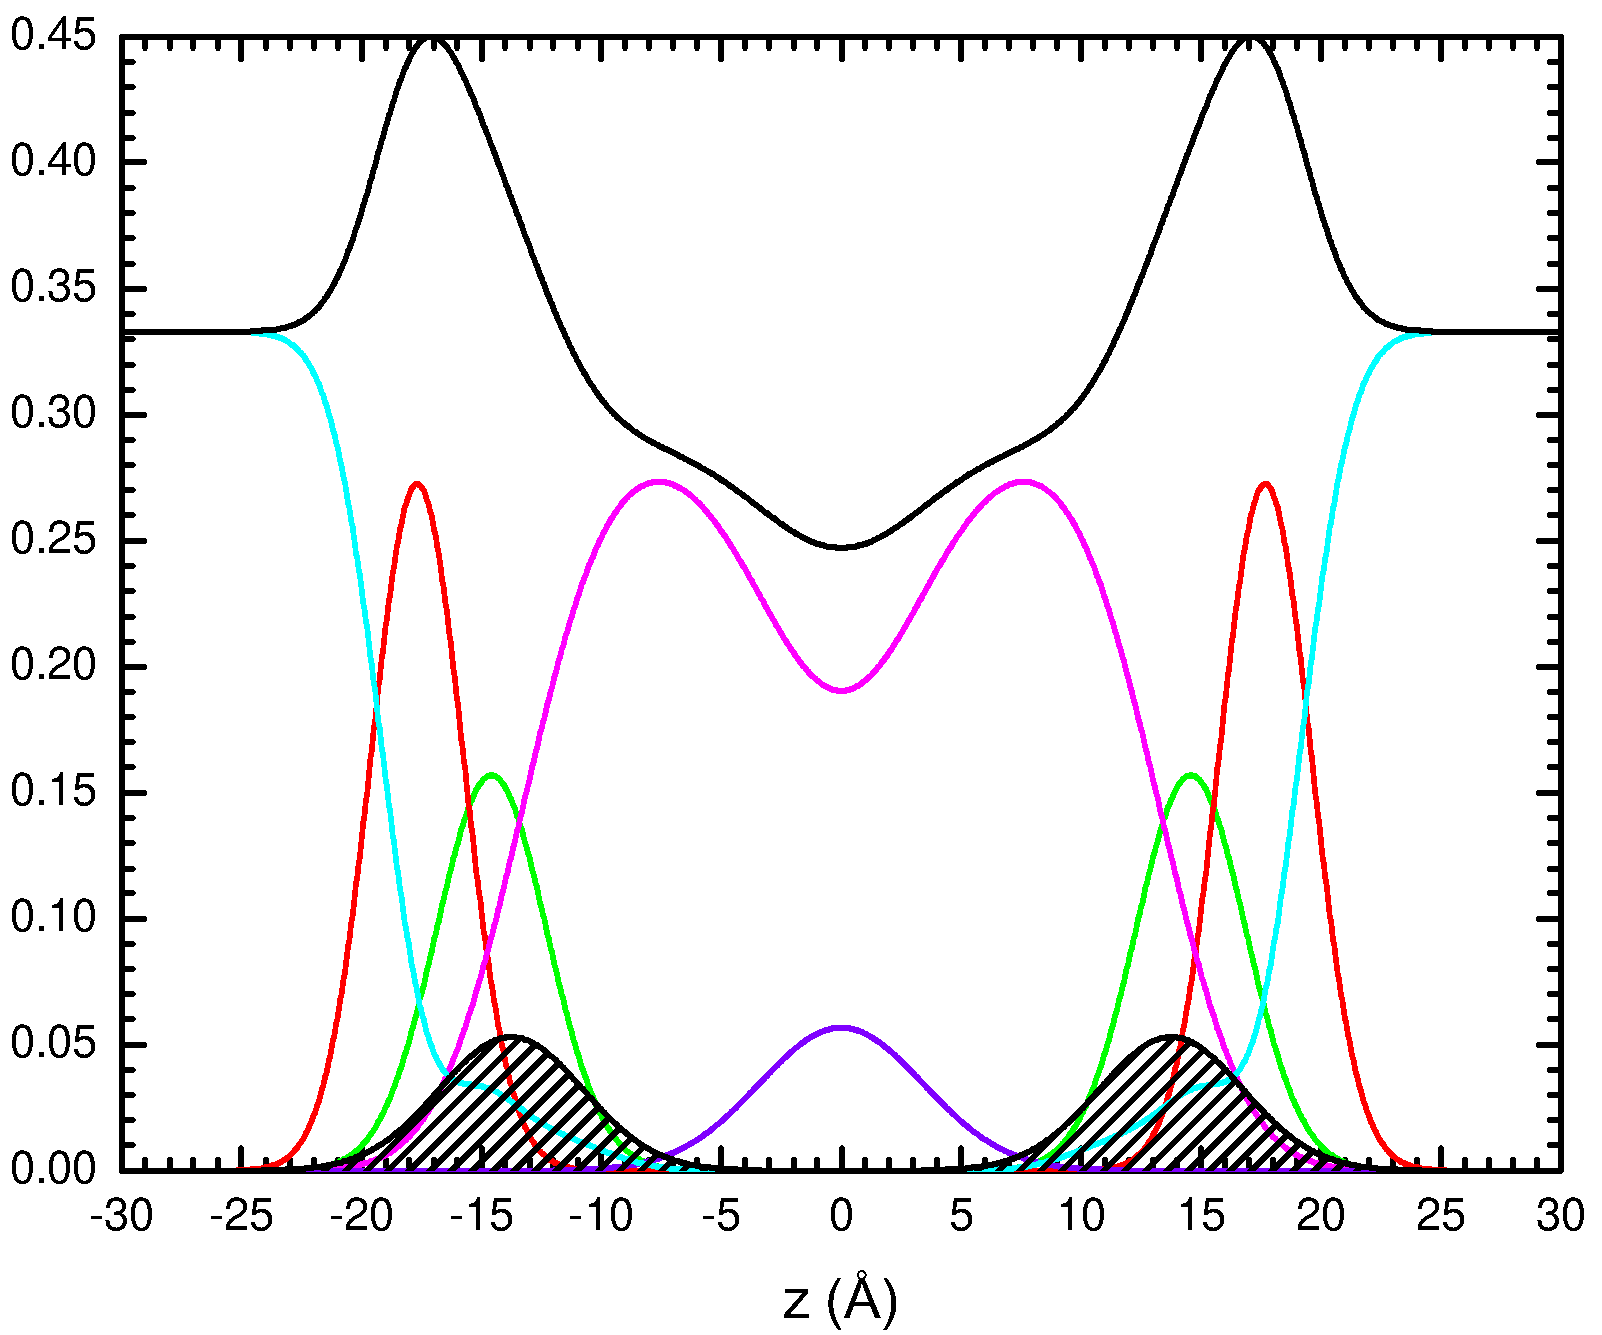
\includegraphics[width=0.45\textwidth,valign=t]{figures/Tat/SDP_Results/EDP/DOPC_Tat_28to1_3p0_EDP1}
  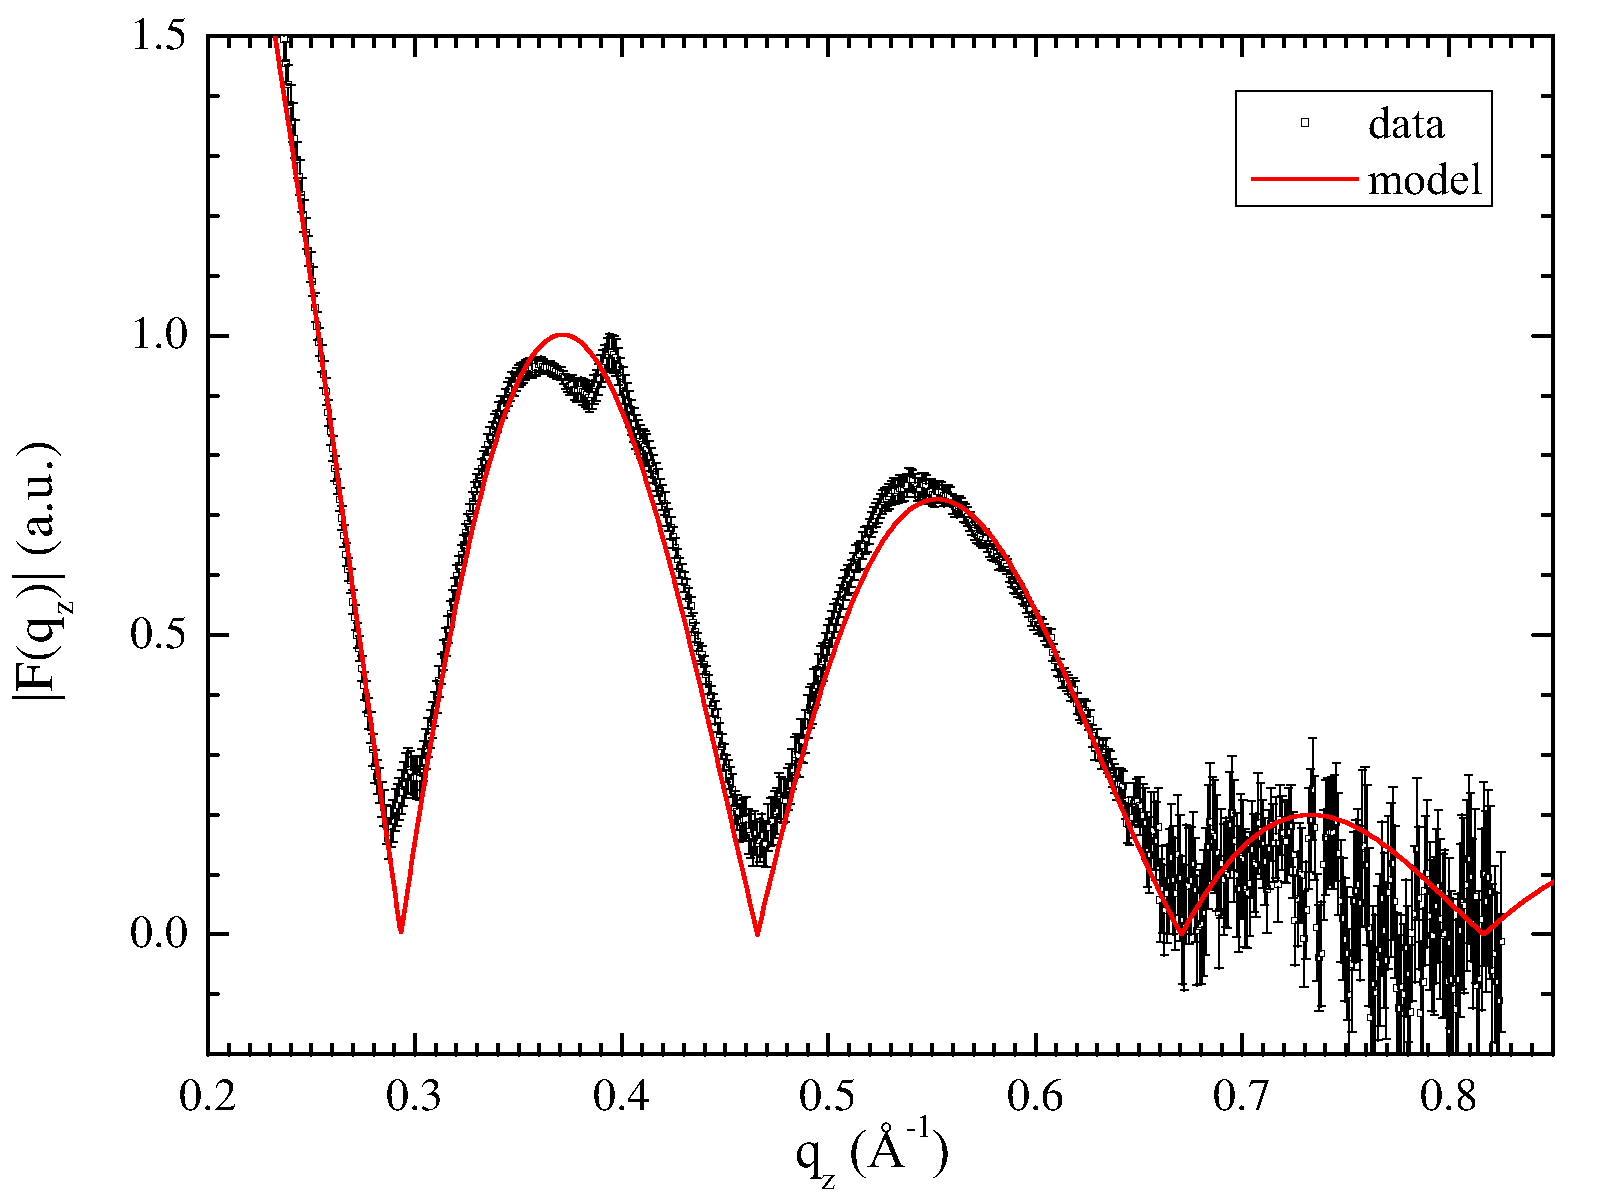
\includegraphics[width=0.45\textwidth,valign=t]{figures/Tat/SDP_Results/XFF/DOPC_Tat_16to1_3p0_XFF1}
  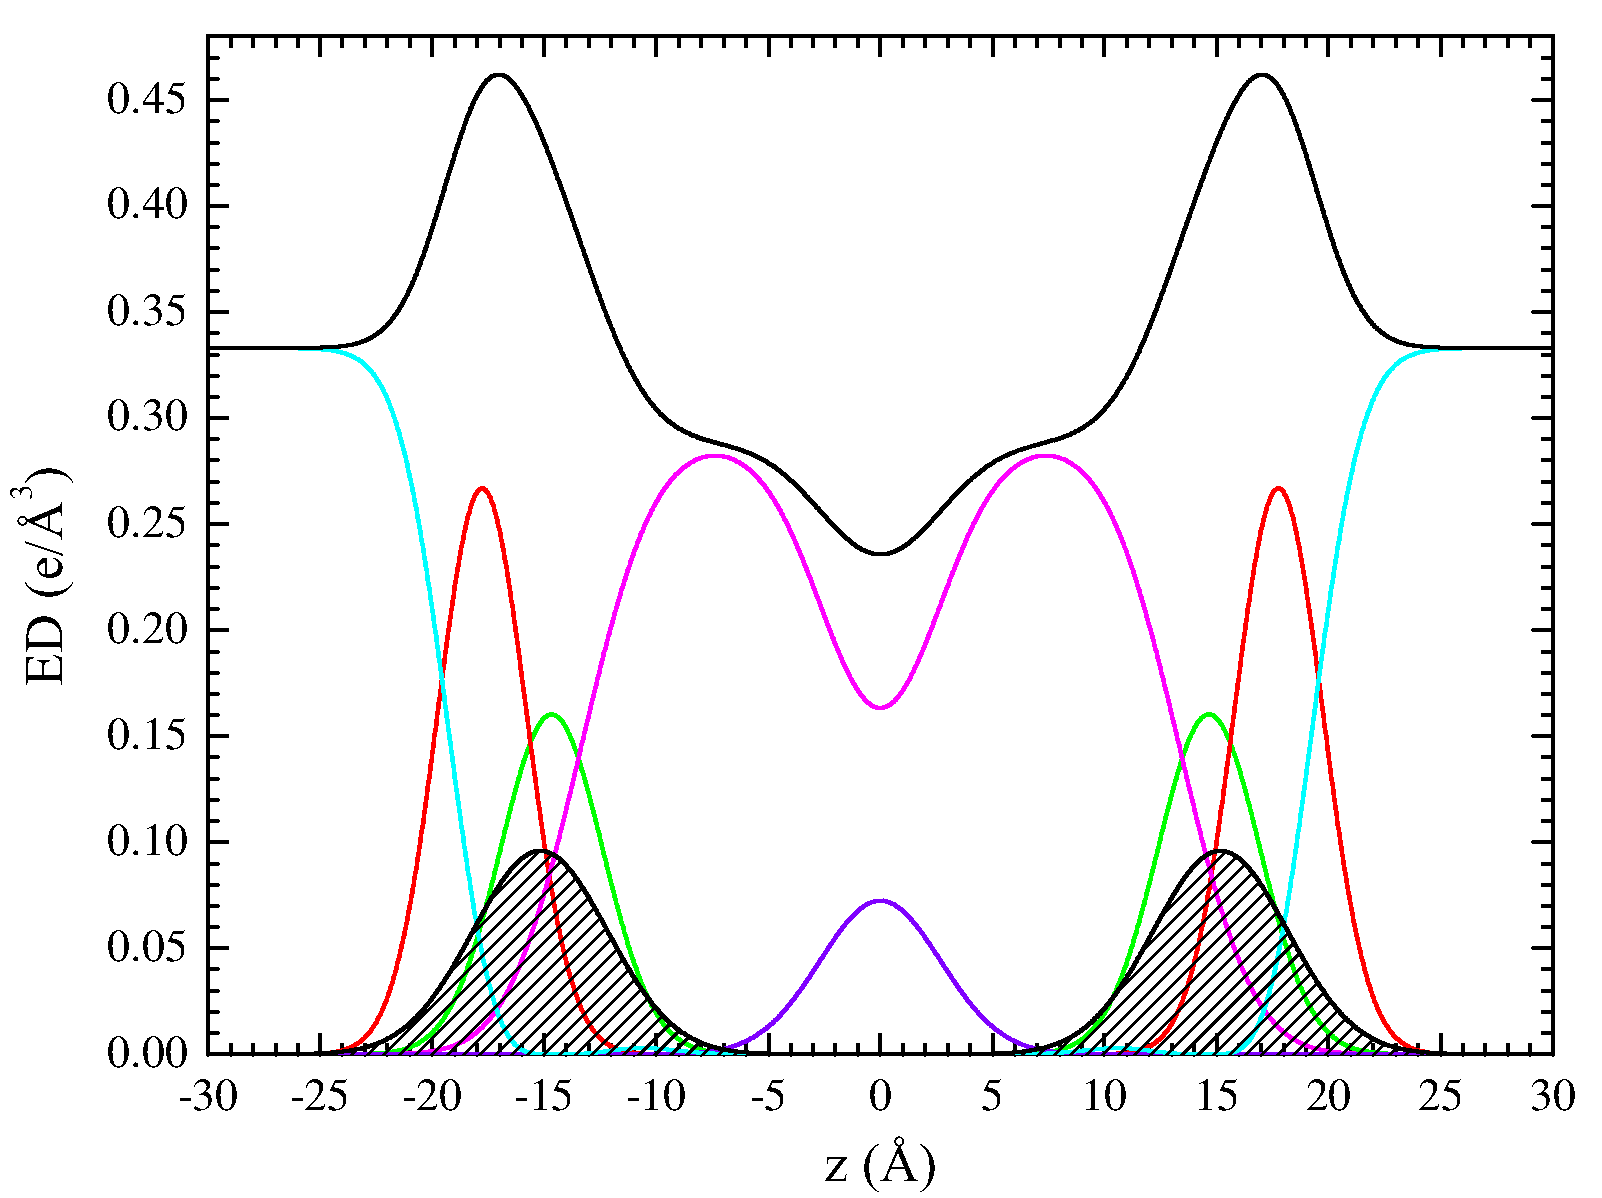
\includegraphics[width=0.45\textwidth,valign=t]{figures/Tat/SDP_Results/EDP/DOPC_Tat_16to1_3p0_EDP1}
  \caption{The best fits to DOPC form factors (left) and the corresponding 
  electron density profiles (right) with $\xTat$ = 0, 0.016, 0.034, 
  and 0.059 (from top to bottom).}
  \label{fig:DOPC_Tat_XFF1}
\end{figure}
%------------------------------------------------------------------------------
\begin{table}[htbp]
  \centering
  \begin{tabular}{|c|c|c|c|c|c|c|c|c|c|c|}
    \hline
    $\xTat$ & 0 & \multicolumn{3}{c|}{1/63} & \multicolumn{3}{c|}{1/29} & \multicolumn{3}{c|}{1/17} \\
    \hline
    $\chi^2$ & 2961 & 1554 & 1570 & 1581 & 1563 & 1587 & 1607 & 2342 & 2338 & 2363 \\ 
    $\chi^2_\textrm{red}$ & 5.307 & 2.785 & 2.813 & 2.833 & 2.807 & 2.849 & 2.885 & 4.197 & 4.189 & 4.235 \\
    \hline
    $\zPC$ & 18.1 & 18.0 & 17.9 & 17.9 & 17.8 & 17.7 & 17.6 & 17.8 & 17.8 & 17.7 \\
    $\sigmaPC$ & 2.52 & 2.14 & 2.17 & 2.18 & 1.86 & 1.92 & 1.93 & 2.02 & 1.97 & 1.93 \\
    $\zCG$ & 15.0 & 14.9 & 14.8 & 14.8 & 14.7 & 14.6 & 14.5 & 14.7 & 14.7 & 14.6 \\
    $\sigmaCG$ & 3.00 & 2.62 & 2.64 & 2.66 & 2.22 & 2.30 & 2.31 & 2.58 & 2.27 & 2.14 \\
    $\zHC$ & 13.7 & 13.6 & 13.5 & 13.5 & 13.4 & 13.3 & 13.2 & 13.4 & 13.4 & 13.3 \\ 
    $\sigmaHC$ & 3.00 & 2.69 & 2.84 & 2.95 & 2.65 & 2.82 & 3.01 & 2.47 & 2.58 & 2.83 \\
    $\sigmaCHthree$ & 3.20 & 3.19 & 3.22 & 3.24 & 3.37 & 3.43 & 3.47 & 2.70 & 2.70 & 2.74 \\
    $\zTat$ & NA & 12.9 & 13.4 & 14.2 & 13.1 & 13.8 & 14.4 & 15.2 & 15.2 & 15.7 \\
    $\sigmaTat$ & NA & 2.5 & 3.0 & 3.5 & 2.5 & 3.0 & 3.5 & 2.5 & 3.0 & 3.5 \\ 
    \hline
    $\VL$ & 1314 & \multicolumn{3}{c|}{1344} & \multicolumn{3}{c|}{1380} & \multicolumn{3}{c|}{1432} \\ 
    $\VHL$ & 331 & \multicolumn{3}{c|}{362} & \multicolumn{3}{c|}{397} & \multicolumn{3}{c|}{450} \\
    $\VTat$ & 0 & \multicolumn{3}{c|}{30.5} & \multicolumn{3}{c|}{66.1} & \multicolumn{3}{c|}{118.8} \\
    $\RPC$ & 0.59 & \multicolumn{3}{c|}{0.54} & \multicolumn{3}{c|}{0.49} & \multicolumn{3}{c|}{0.43} \\
    $\RCG$ & 0.41 & \multicolumn{3}{c|}{0.38} & \multicolumn{3}{c|}{0.0.34} & \multicolumn{3}{c|}{0.30} \\
    \hline
    $\Delta z_1$ & \multicolumn{10}{c|}{3.1} \\
    $\Delta z_2$ & \multicolumn{10}{c|}{1.3} \\
    $\rCHthree$ & \multicolumn{10}{c|}{1.97} \\
    $\rTat$ & \multicolumn{10}{c|}{0} \\
    \hline
    $\AL$ & 71.5 & 72.4 & 72.5 & 72.7 & 73.6 & 74.0 & 74.4 & 73.6 & 73.5 & 73.9 \\
    \hline
  \end{tabular}
  \caption{Fitting Results for DOPC membranes. $\Delta z_1 = \zPC-\zCG$
  and $\Delta z_2 = \zCG-\zHC$.}
  \label{tb:DOPC_fit_results}
\end{table}
%------------------------------------------------------------------------------

As shown in Fig.~\ref{fig:DOPC_Tat_XFF1}, the membrane thickness can be defined
as the distance $\DPP$ between the PC components in the opposing leaflets
or the distance $\DHH$ between the maxima in the opposing leaflets. $\DHH$
is more reliable than $\DPP$ because it is a property of the total 
electron density of a bilayer and, therefore, does not depend strongly on the 
specific model employed for fitting the data. Indeed, the total electron
density profile can be determined independently of a bilayer model 
by writing the electron density profile in terms of Fourier series, Fourier transforming
the profile, and fitting the resulting model independent
form factor to the data. On the other hand, $\DPP$ is a property that
depends on lipid components, which are influenced by how the lipid is parsed 
and what assumptions and constraints go into the specific model.
A disadvantage of using $\DHH$ as a measure of the membrane thickness is
that $\DHH$ is influenced by the electron density of Tat because 
the total electron density profile has a contribution from the electron density of Tat. 
Especially when the mole fraction of Tat in a system becomes large, 
the Tat electron density contributes significantly to the total electron 
density profile. If the Tat resided slightly 
outside of the PC component, the apparent membrane thickness measured by $\DHH$
would be larger than $\DPP$. Then, even if the actual bilayer thickness defined by $\DPP$ 
was reduced by the presence of Tat, the effect of thinning might not be obvious. 
With the above caveat in mind, we report both quantities in what follows
since they can be easily calculated from the model.

%------------------------------------------------------------------------------
\begin{figure}[htbp]
  \centering
  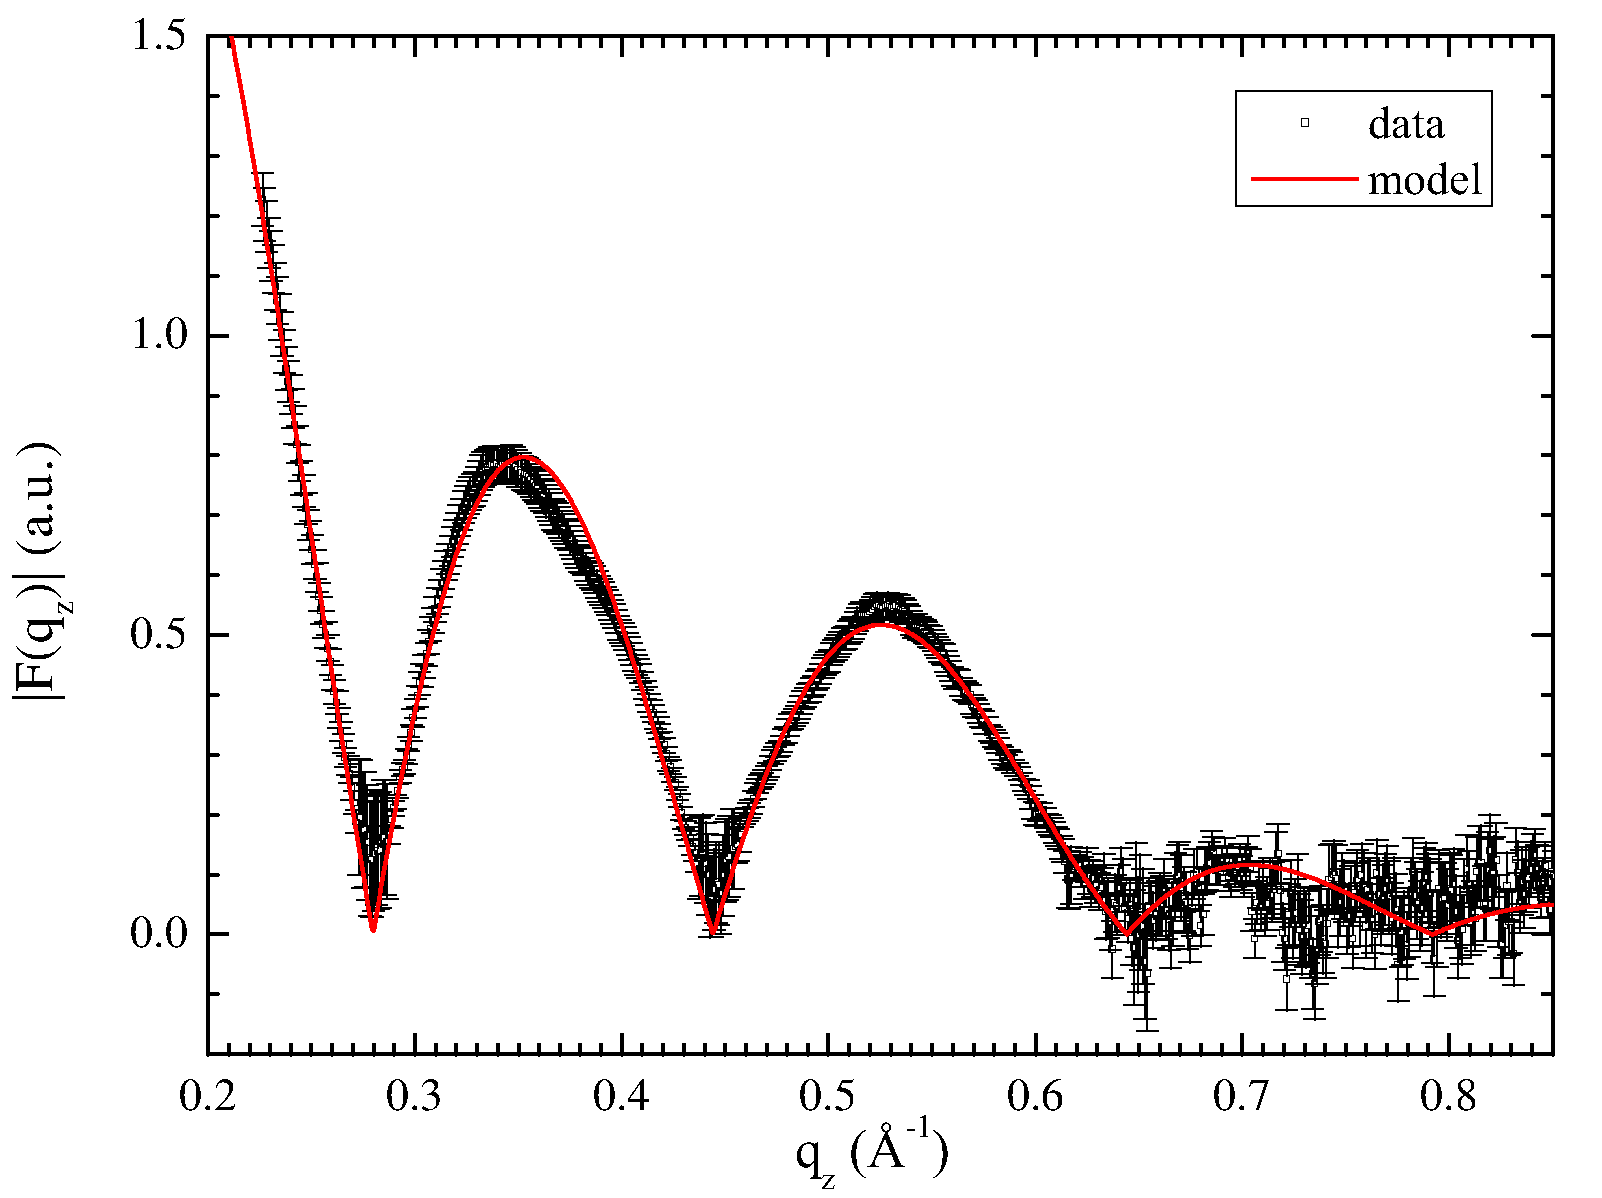
\includegraphics[width=0.45\textwidth,valign=t]{figures/Tat/SDP_Results/XFF/DOPCDOPE3to1_XFF1}
  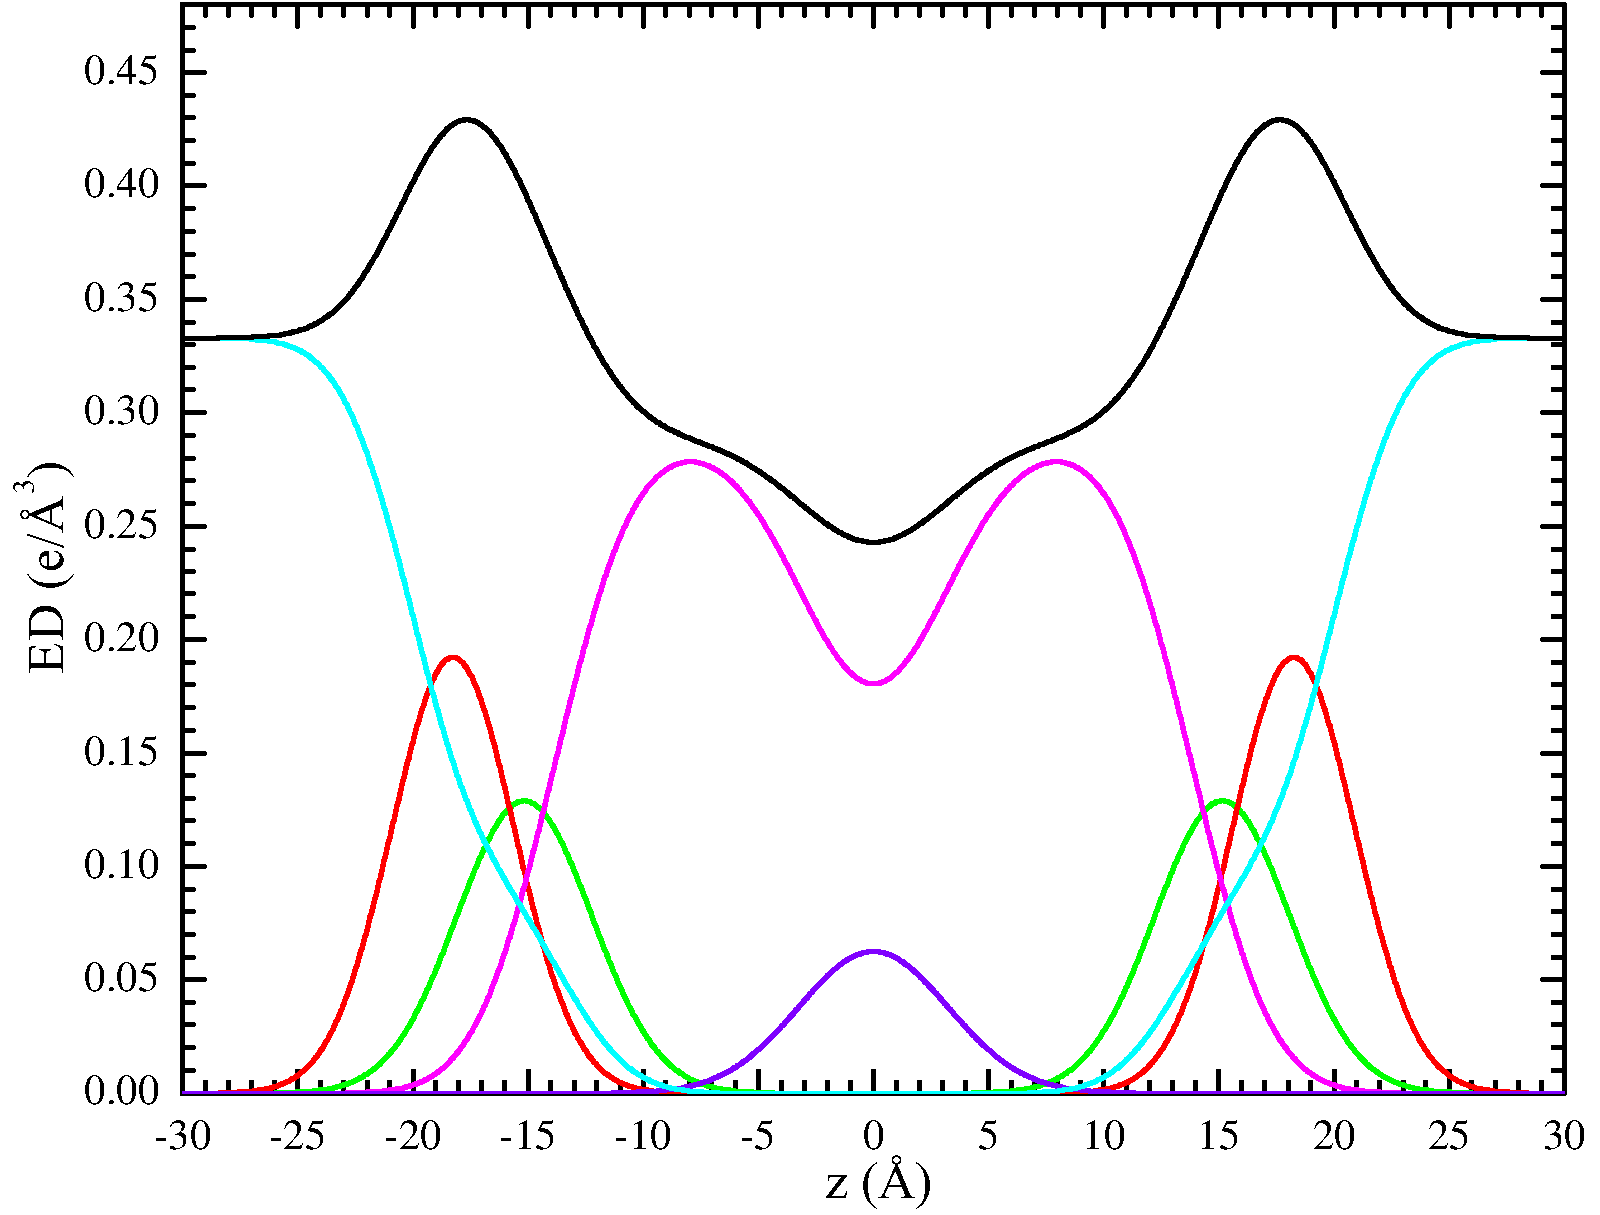
\includegraphics[width=0.45\textwidth,valign=t]{./figures/Tat/SDP_Results/EDP/DOPCDOPE3to1_EDP1}
  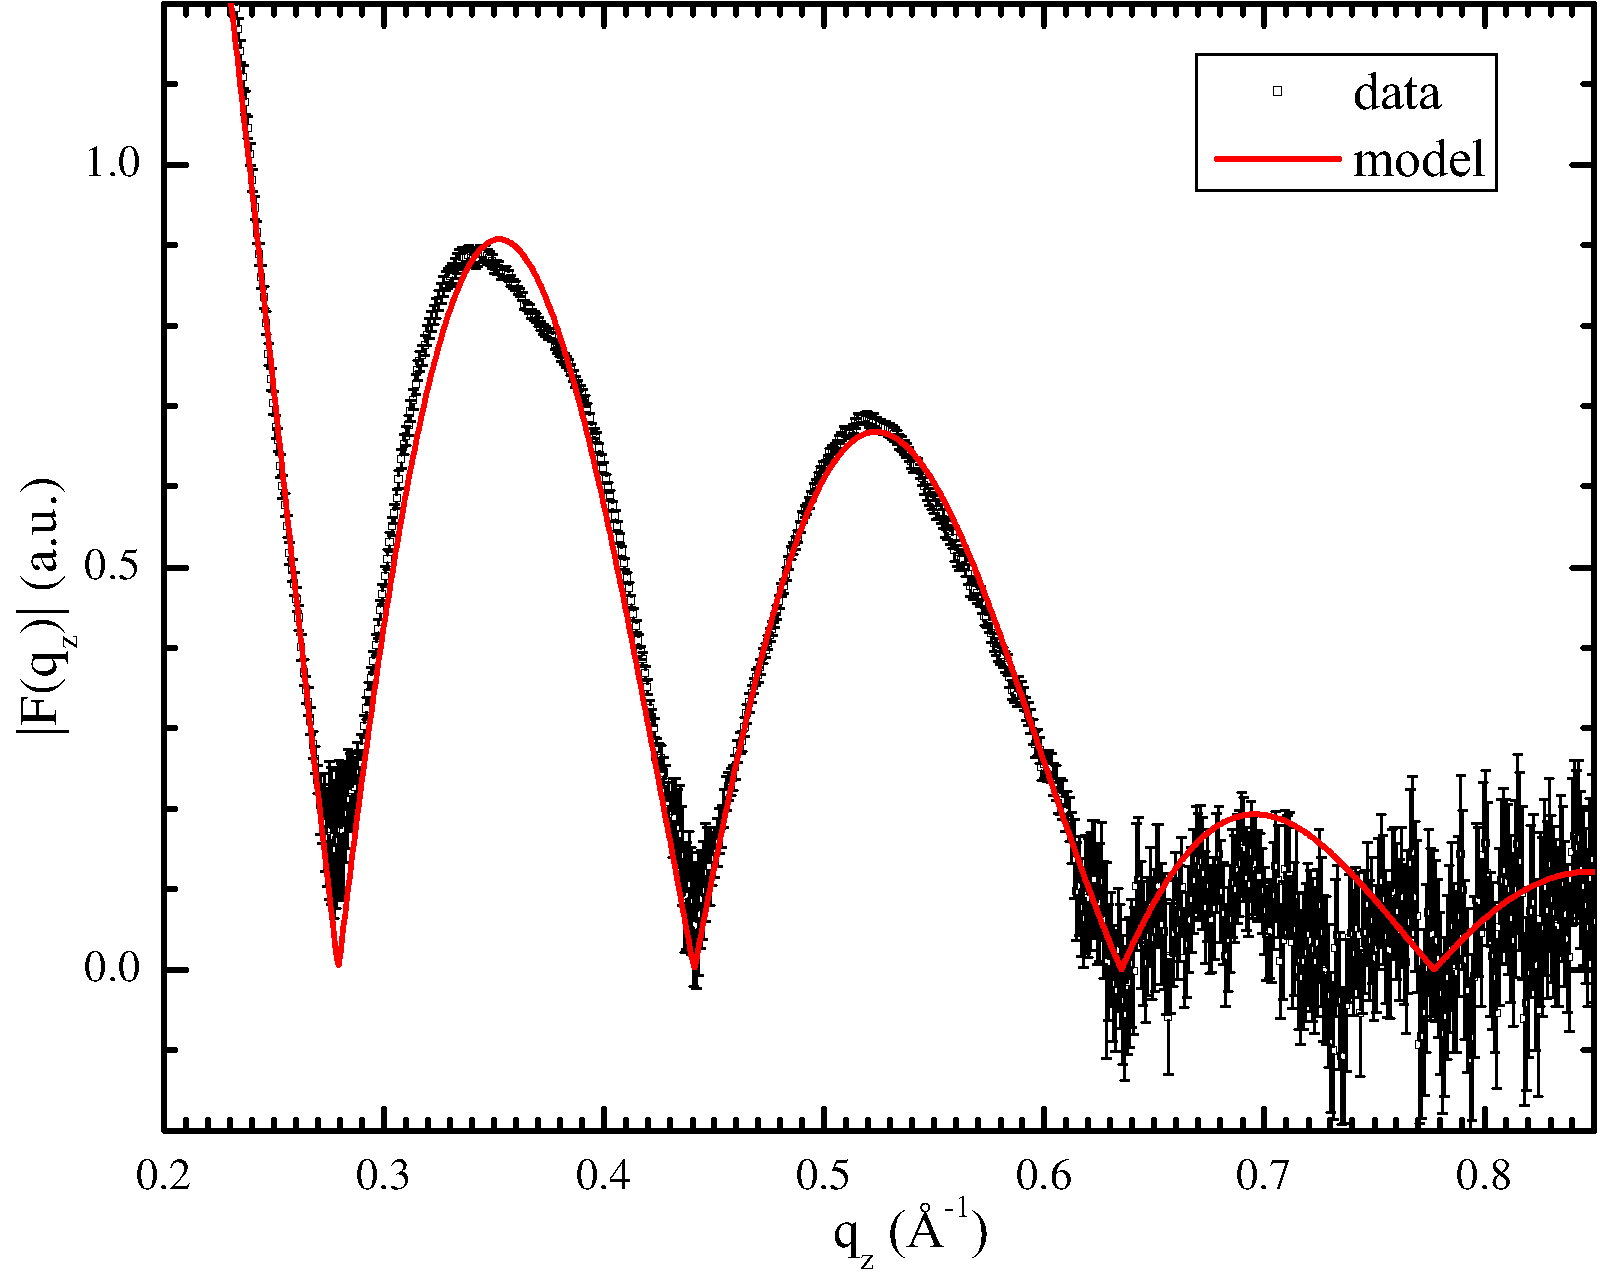
\includegraphics[width=0.45\textwidth,valign=t]{figures/Tat/SDP_Results/XFF/DOPCDOPE3to1_Tat_62to1_3p0_XFF1}
  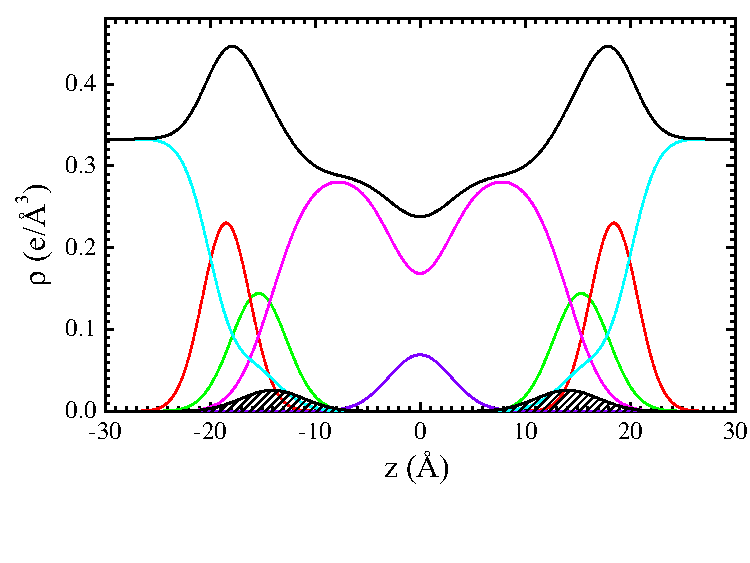
\includegraphics[width=0.45\textwidth,valign=t]{./figures/Tat/SDP_Results/EDP/DOPCDOPE3to1_Tat_62to1_3p0_EDP1}
  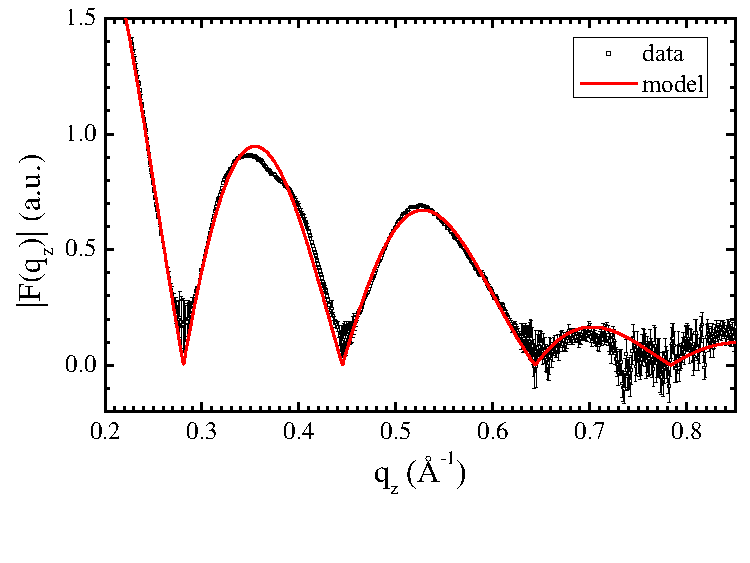
\includegraphics[width=0.45\textwidth,valign=t]{figures/Tat/SDP_Results/XFF/DOPCDOPE3to1_Tat_28to1_3p0_XFF1}
  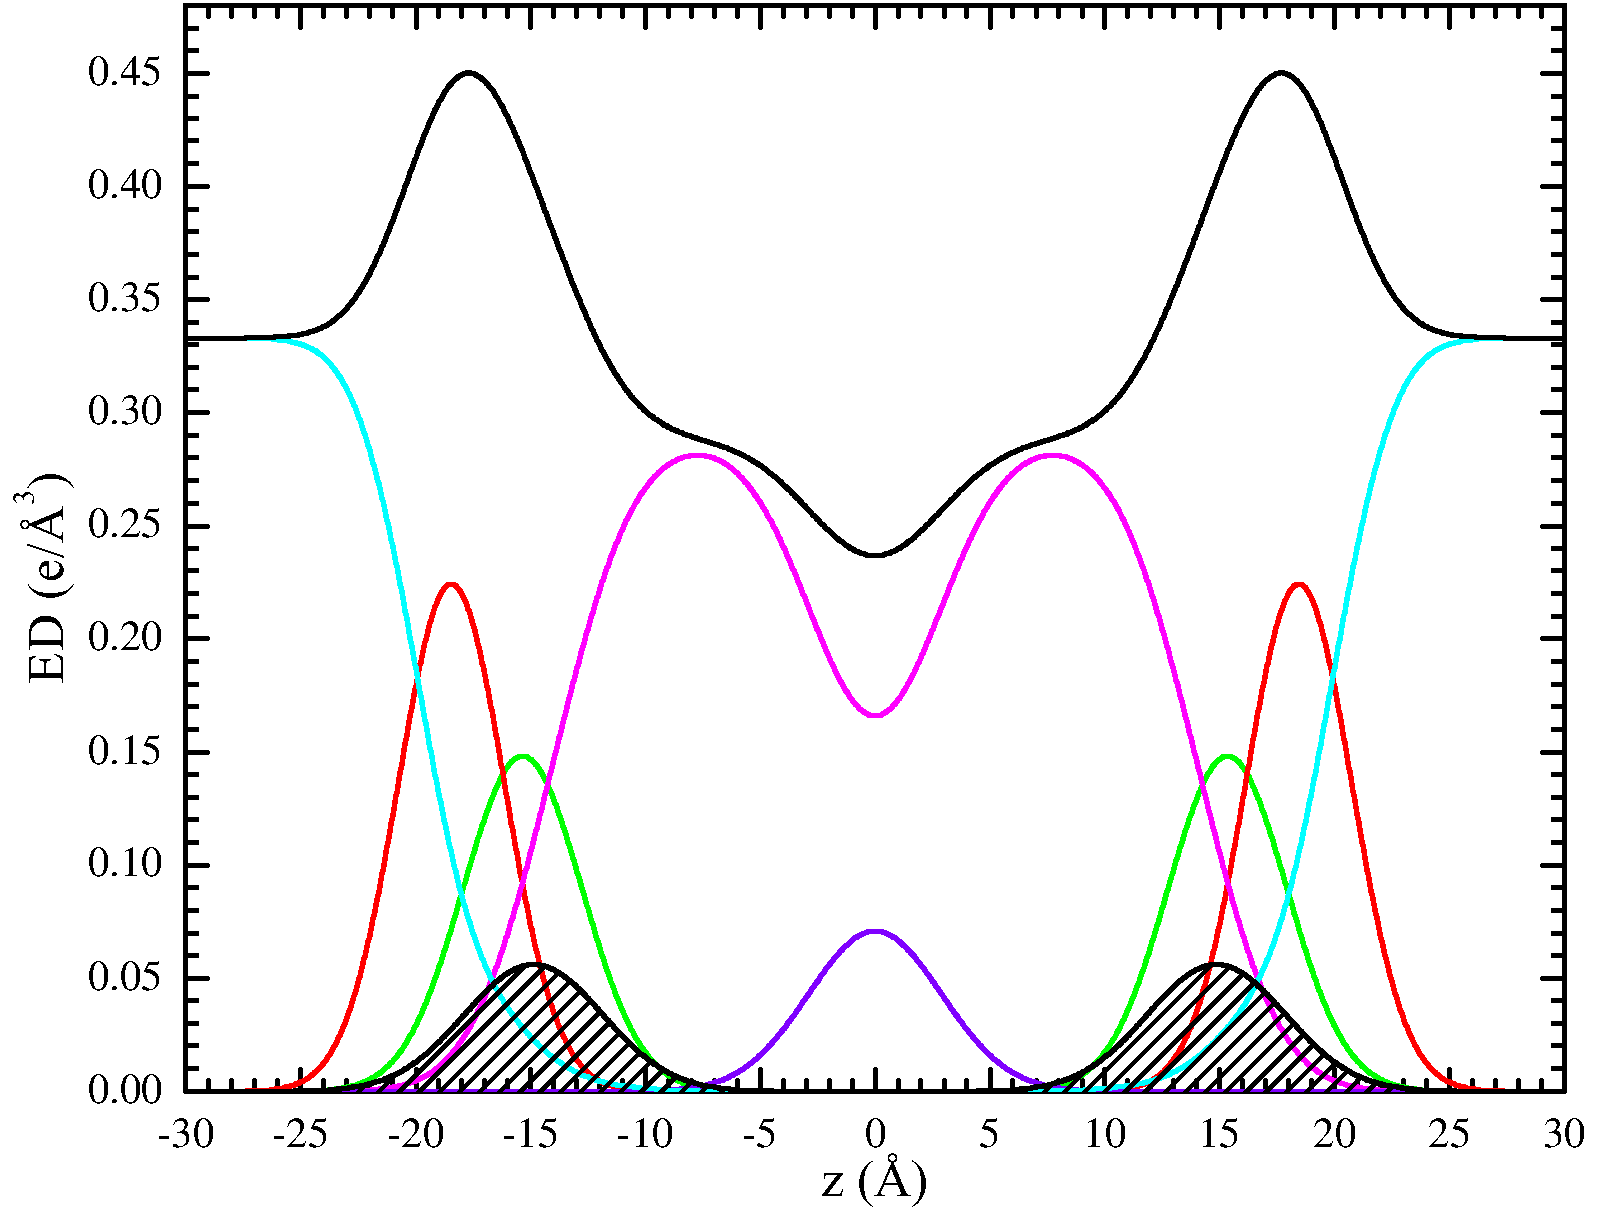
\includegraphics[width=0.45\textwidth,valign=t]{./figures/Tat/SDP_Results/EDP/DOPCDOPE3to1_Tat_28to1_3p0_EDP1}
  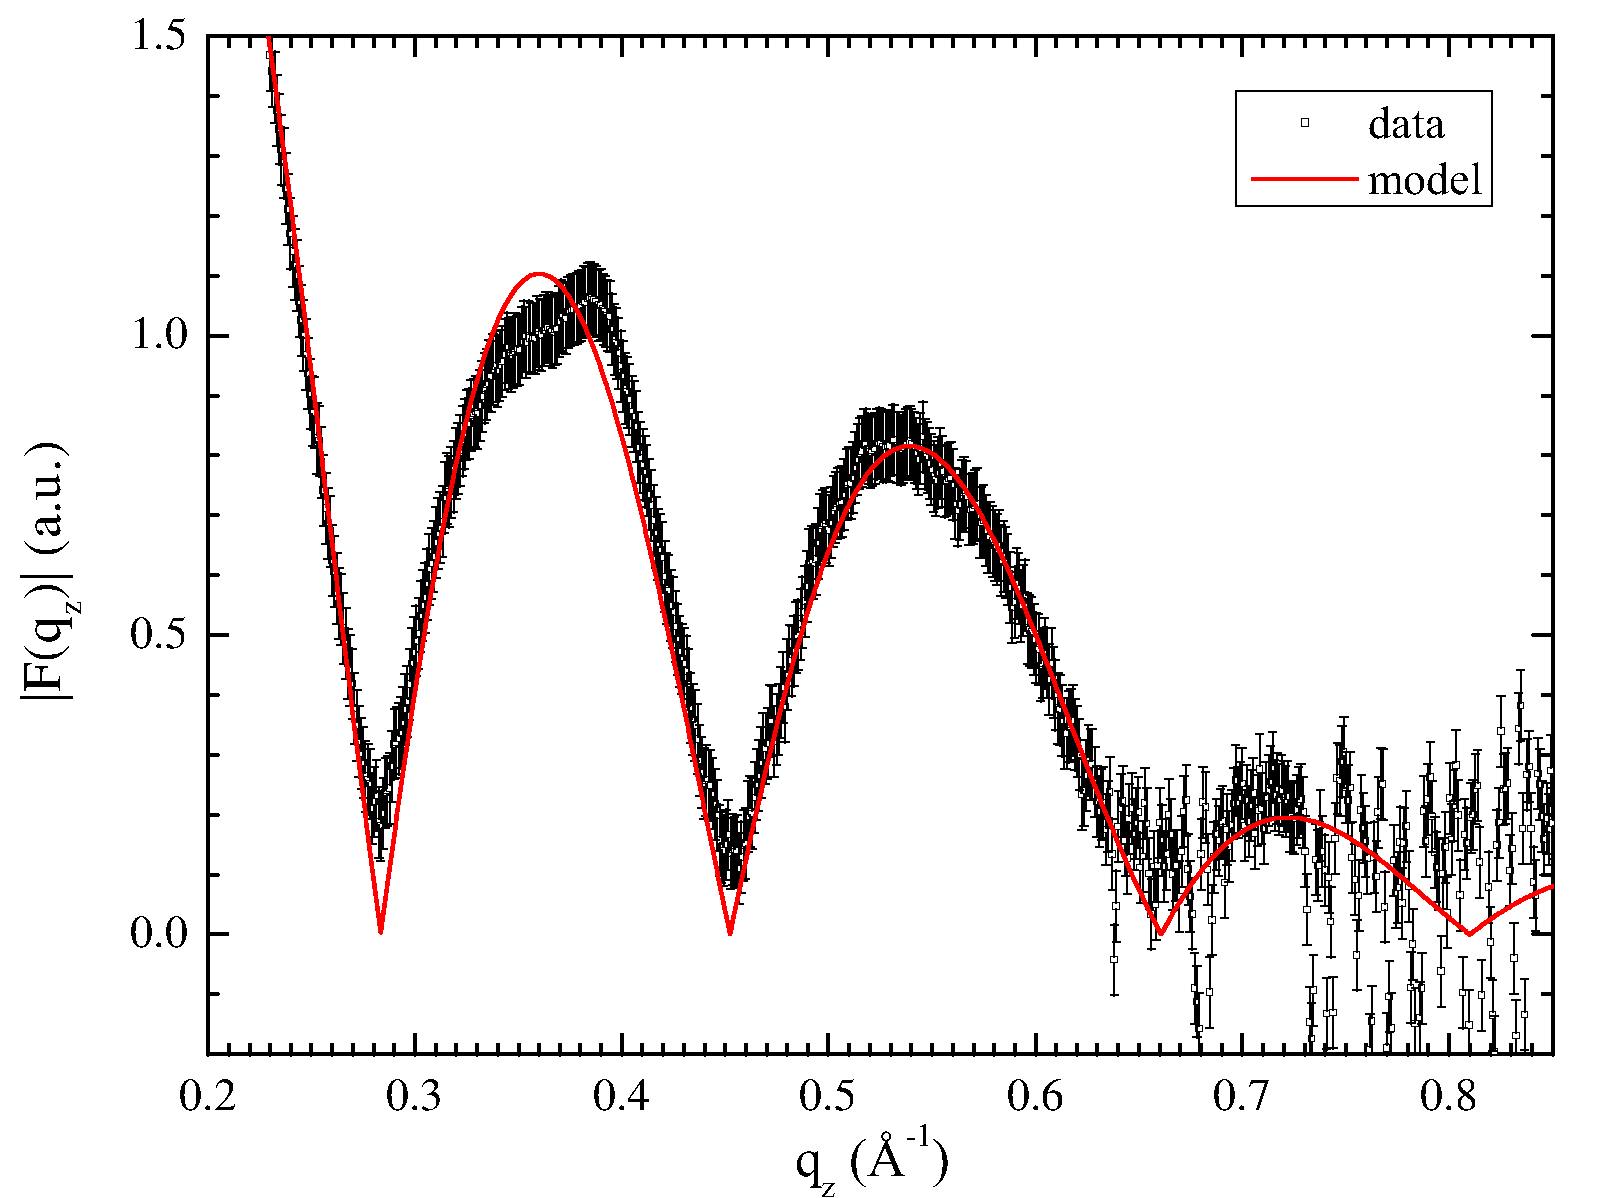
\includegraphics[width=0.45\textwidth,valign=t]{figures/Tat/SDP_Results/XFF/DOPCDOPE3to1_Tat_16to1_3p0_XFF1}
  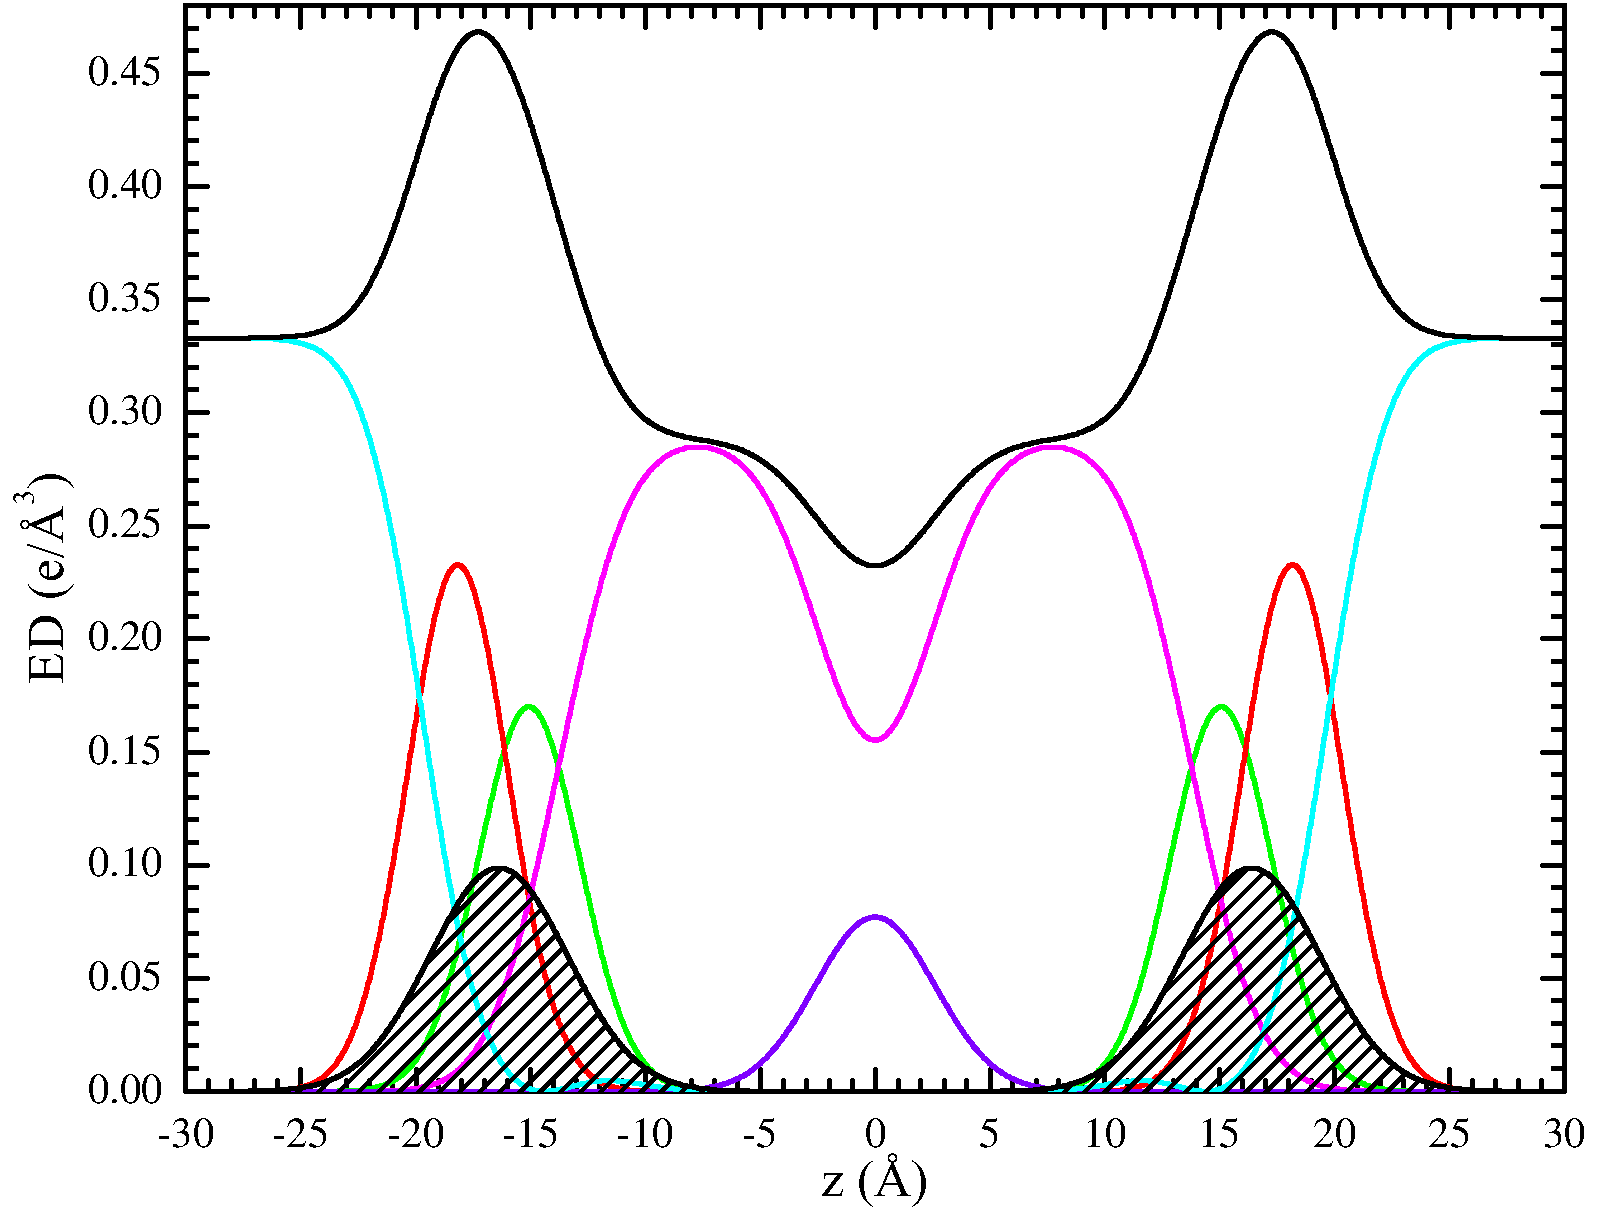
\includegraphics[width=0.45\textwidth,valign=t]{./figures/Tat/SDP_Results/EDP/DOPCDOPE3to1_Tat_16to1_3p0_EDP1}
  \caption{The best fits to DOPC:DOPE (3:1) form factors (left) and the corresponding 
  electron density profiles (right) with $\xTat$ = 0, 0.016, 0.034, 
  and 0.059 (from top to bottom).}
  \label{fig:DOPCDOPE3to1_Tat_XFF1}
\end{figure}
%------------------------------------------------------------------------------
\begin{table}[htbp]
  \centering
  \begin{tabular}{|c|c|c|c|c|c|c|c|c|c|c|}
    \hline
    $\xTat$ & 0 & \multicolumn{3}{c|}{1/63} & \multicolumn{3}{c|}{1/29} & \multicolumn{3}{c|}{1/17} \\
    \hline
    $\chi^2$ & 924.5 & 4972 & 4985 & 4994 & 6758 & 6826 & 6863 & 2293 & 2280 & 2296 \\ 
    \hline
    $\zPC$ & 18.3 & 18.5 & 18.5 & 18.4 & 18.5 & 18.4 & 18.3 & 18.2 & 18.2 & 18.1 \\
    $\sigmaPC$ & 2.66 & 2.23 & 2.26 & 2.27 & 2.25 & 2.31 & 2.34 & 2.31 & 2.19 & 2.11 \\
    $\zCG$ & 15.2 & 15.4 & 15.4 & 15.3 & 15.4 & 15.3 & 15.2 & 15.1 & 15.1 & 15.0 \\
    $\sigmaCG$ & 2.92 & 2.63 & 2.65 & 2.69 & 2.52 & 2.58 & 2.63 & 2.40 & 2.20 & 2.01 \\
    $\zHC$ & 13.9 & 14.1 & 14.1 & 14.0 & 14.1 & 14.0 & 13.9 & 13.8 & 13.8 & 13.7 \\
    $\sigmaHC$ & 2.73 & 2.70 & 2.83 & 2.91 & 2.86 & 2.79 & 2.84 & 2.25 & 2.38 & 2.60 \\
    $\sigmaCHthree$ & 3.24 & 2.94 & 2.97 & 2.98 & 2.87 & 2.90 & 2.91 & 2.63 & 2.61 & 2.65 \\
    $\zTat$ & NA & 13.5 & 14.0 & 15.0 & 14.3 & 14.9 & 16.0 & 16.3 & 16.4 & 16.9 \\
    $\sigmaTat$ & NA & 2.5 & 3.0 & 3.5 & 2.5 & 3.0 & 3.5 & 2.5 & 3.0 & 3.5 \\ 
    \hline
    $\VL$ & 1288 & \multicolumn{3}{c|}{1319} & \multicolumn{3}{c|}{1354} & \multicolumn{3}{c|}{1407} \\ 
    $\VHL$ & 306 & \multicolumn{3}{c|}{336} & \multicolumn{3}{c|}{372} & \multicolumn{3}{c|}{425} \\
    $\VTat$ & 0 & \multicolumn{3}{c|}{30.5} & \multicolumn{3}{c|}{66.1} & \multicolumn{3}{c|}{118.8} \\
    $\RPC$ & 0.59 & \multicolumn{3}{c|}{0.54} & \multicolumn{3}{c|}{0.49} & \multicolumn{3}{c|}{0.43} \\
    $\RCG$ & 0.41 & \multicolumn{3}{c|}{0.38} & \multicolumn{3}{c|}{0.0.34} & \multicolumn{3}{c|}{0.30} \\
    \hline
    $\Delta z_1$ & \multicolumn{10}{c|}{3.1} \\
    $\Delta z_2$ & \multicolumn{10}{c|}{1.3} \\
    $\rCHthree$ & \multicolumn{10}{c|}{1.97} \\
    $\rTat$ & \multicolumn{10}{c|}{0} \\
    \hline
    $\AL$ & 70.9 & 69.8 & 69.9 & 70.1 & 69.5 & 70.0 & 70.6 & 71.3 & 71.4 & 71.7 \\
    \hline
  \end{tabular}
  \caption{Fitting Results for DOPC:DOPE (3:1) membranes. $\Delta z_1 = \zPC-\zCG$
  and $\Delta z_2 = \zCG-\zHC$.}
  \label{tb:DOPCDOPE3to1_fit_results}
\end{table}
%------------------------------------------------------------------------------


%------------------------------------------------------------------------------
\begin{figure}[htbp]
  \centering
  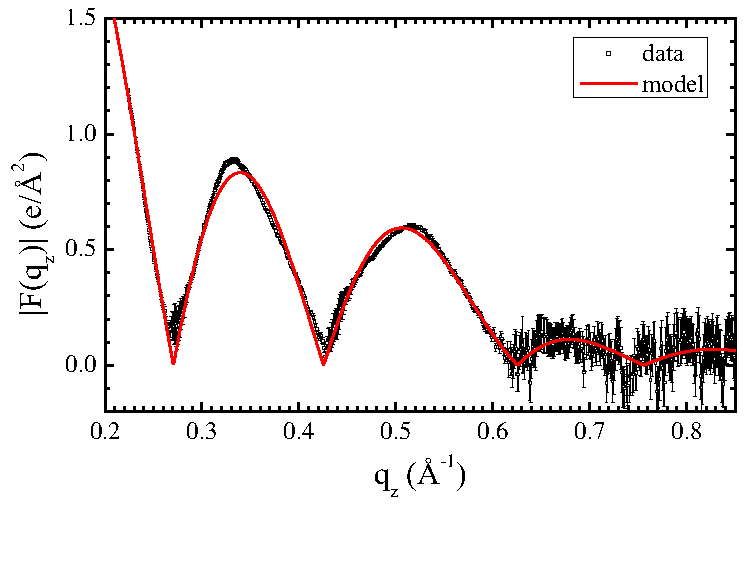
\includegraphics[width=0.45\textwidth,valign=t]{figures/Tat/SDP_Results/XFF/DOPCDOPE1to1_XFF1}
  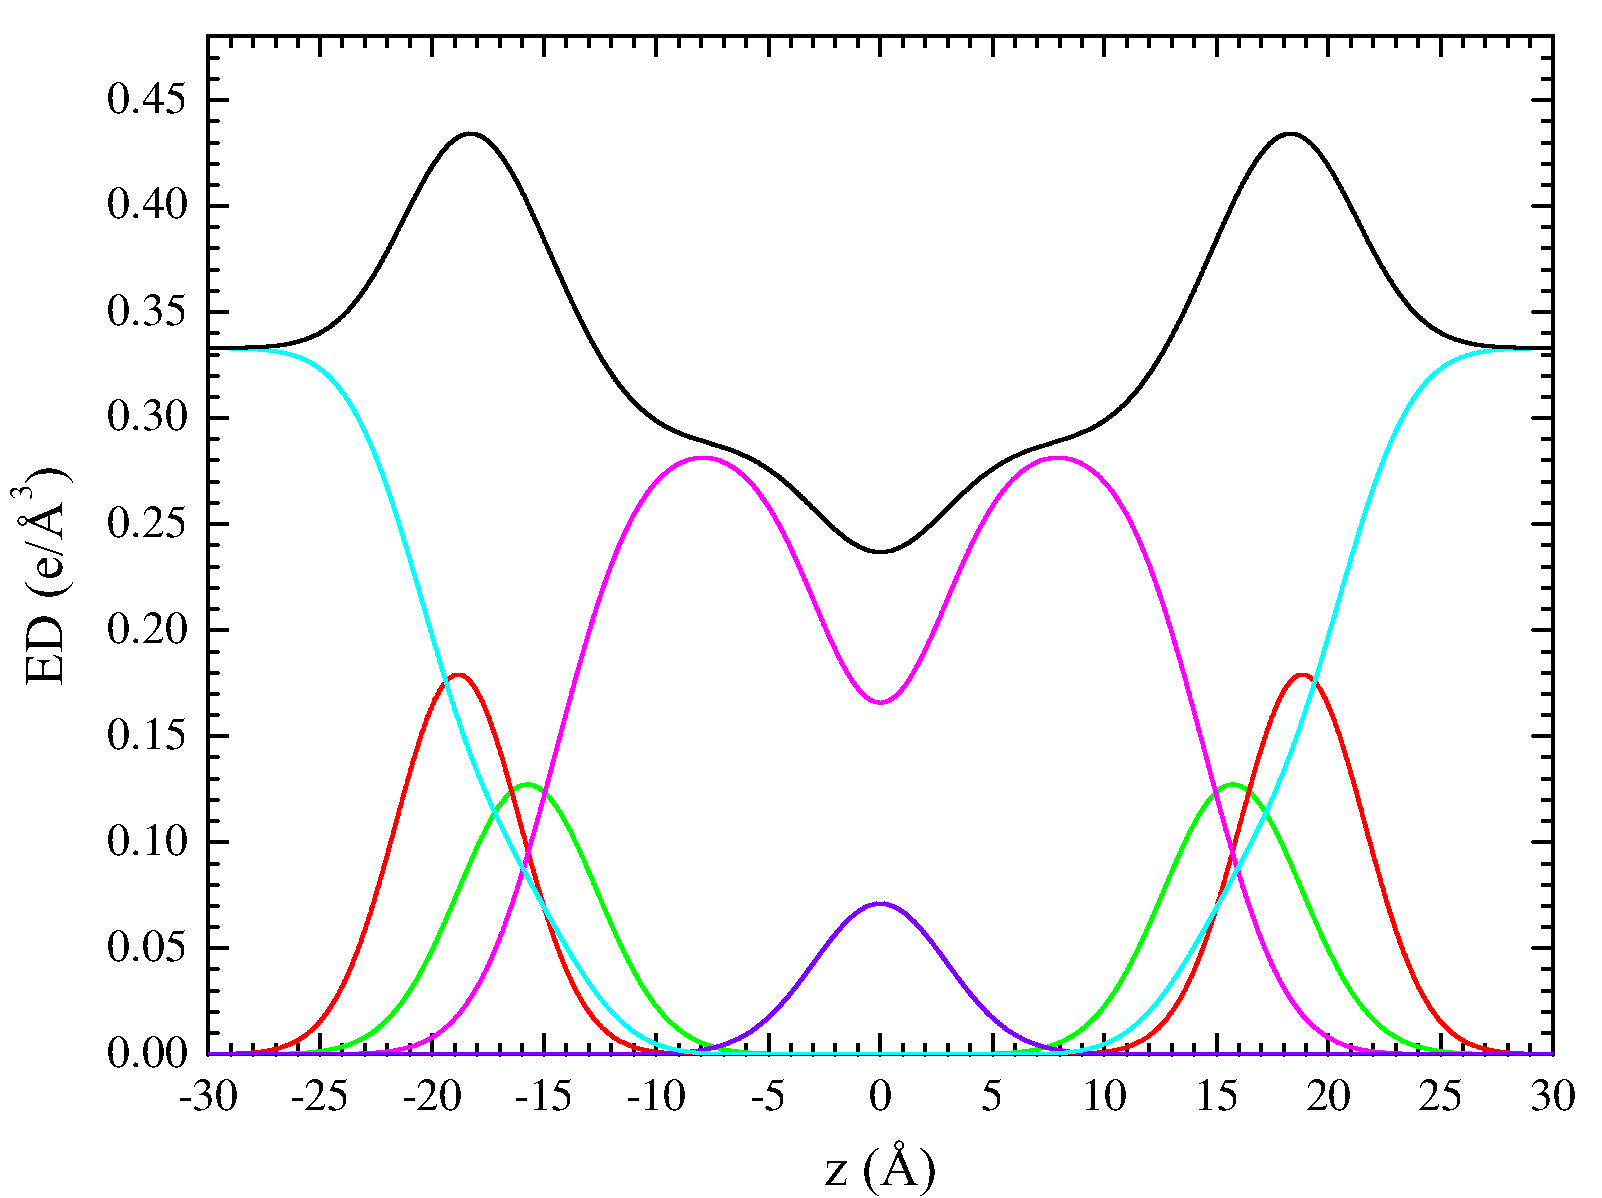
\includegraphics[width=0.45\textwidth,valign=t]{./figures/Tat/SDP_Results/EDP/DOPCDOPE1to1_EDP1}
  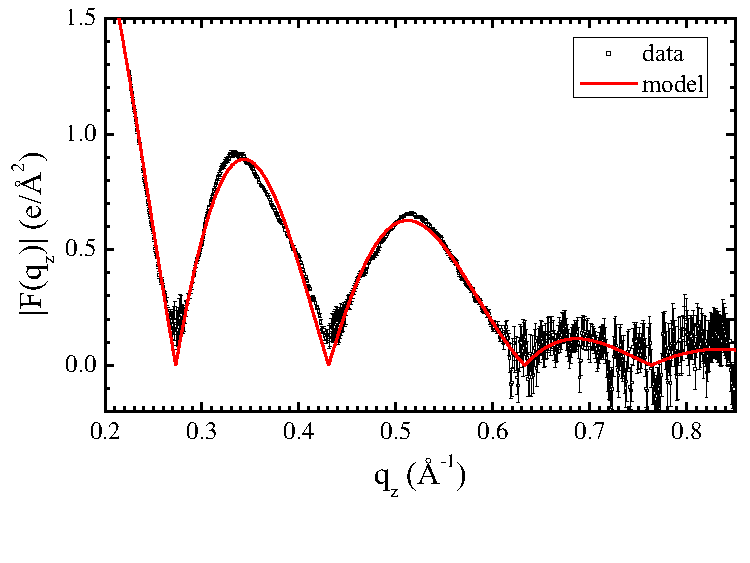
\includegraphics[width=0.45\textwidth,valign=t]{figures/Tat/SDP_Results/XFF/DOPCDOPE1to1_Tat_62to1_3p0_XFF1}
  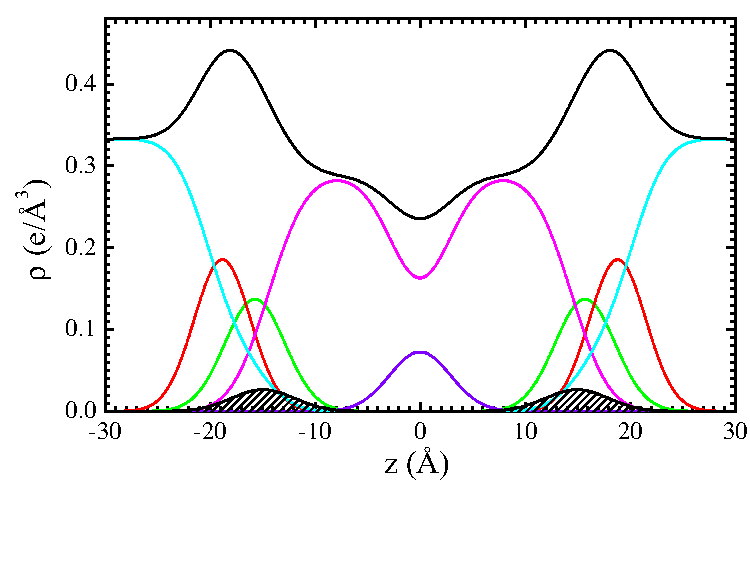
\includegraphics[width=0.45\textwidth,valign=t]{./figures/Tat/SDP_Results/EDP/DOPCDOPE1to1_Tat_62to1_3p0_EDP1}
  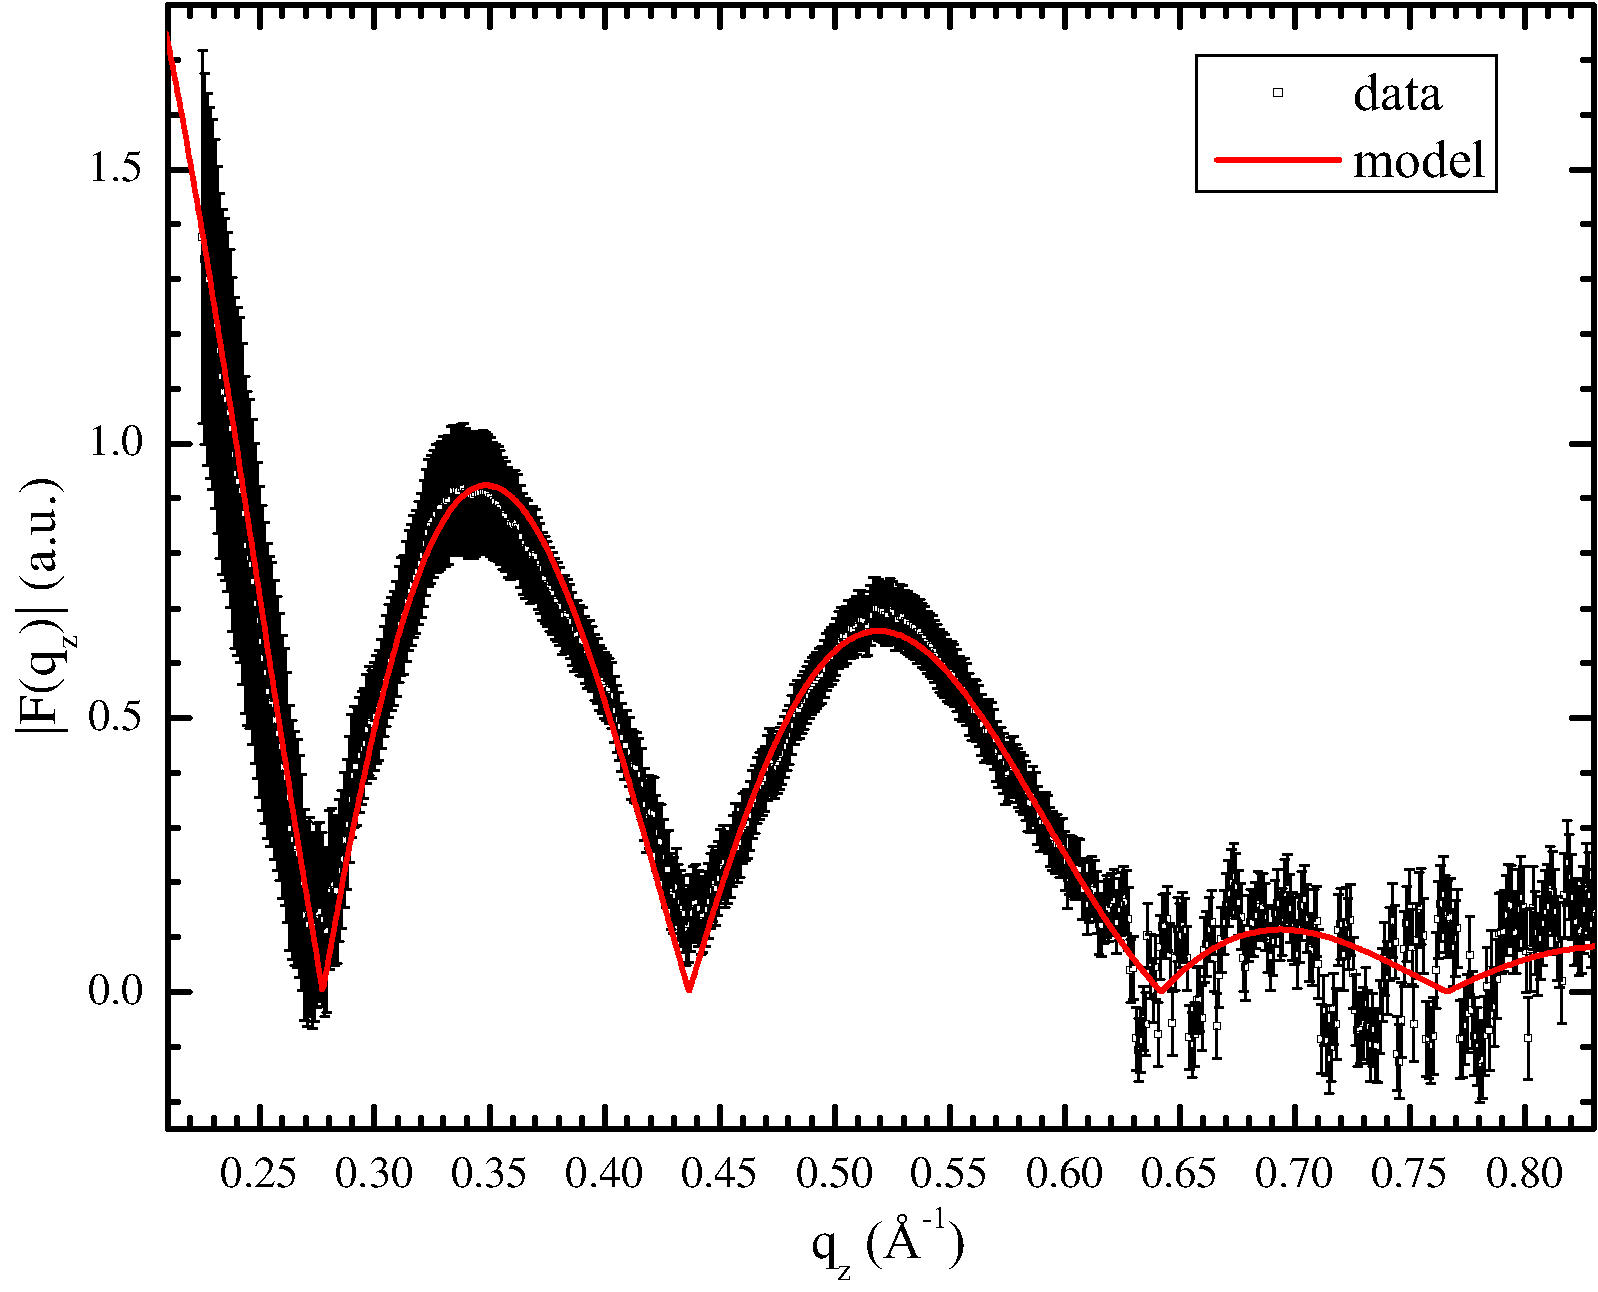
\includegraphics[width=0.45\textwidth,valign=t]{figures/Tat/SDP_Results/XFF/DOPCDOPE1to1_Tat_28to1_3p0_XFF1}
  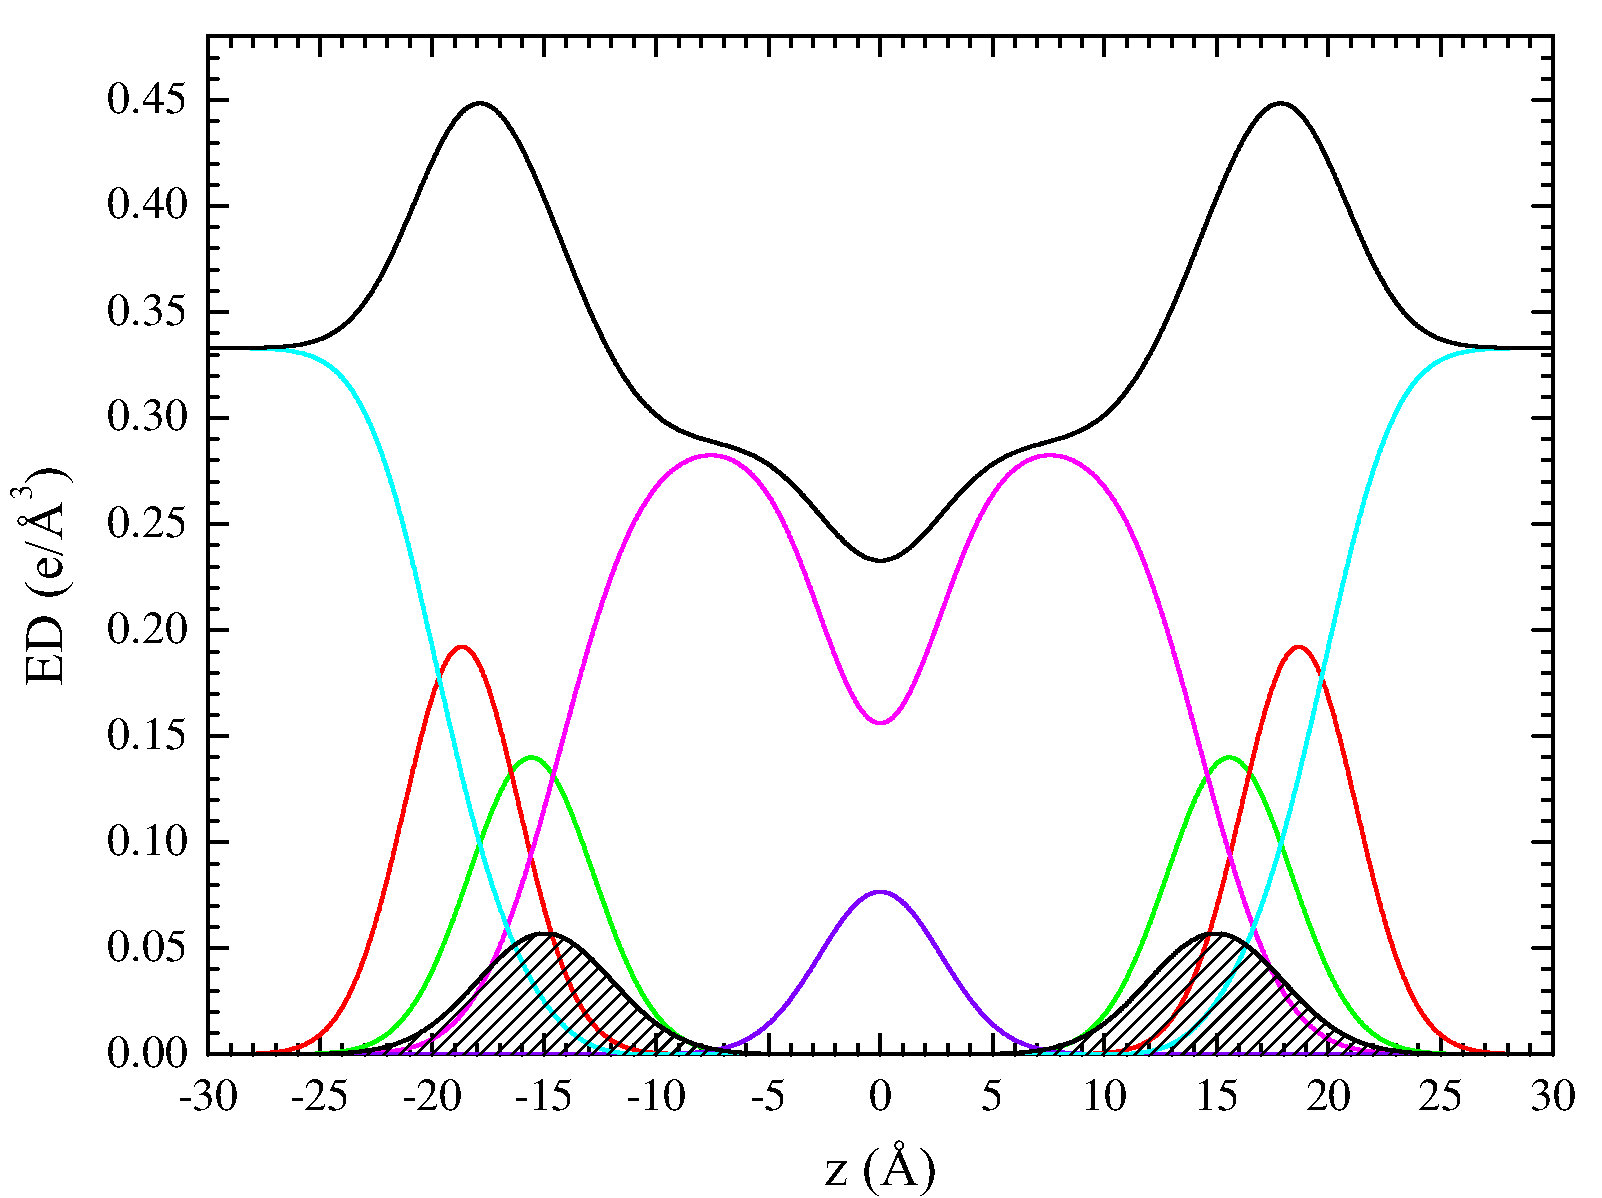
\includegraphics[width=0.45\textwidth,valign=t]{./figures/Tat/SDP_Results/EDP/DOPCDOPE1to1_Tat_28to1_3p0_EDP1}
  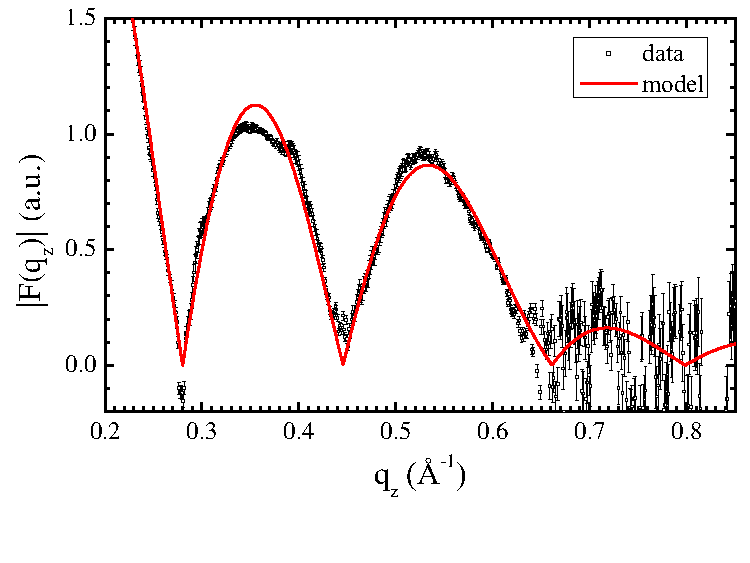
\includegraphics[width=0.45\textwidth,valign=t]{figures/Tat/SDP_Results/XFF/DOPCDOPE1to1_Tat_16to1_3p0_XFF1}
  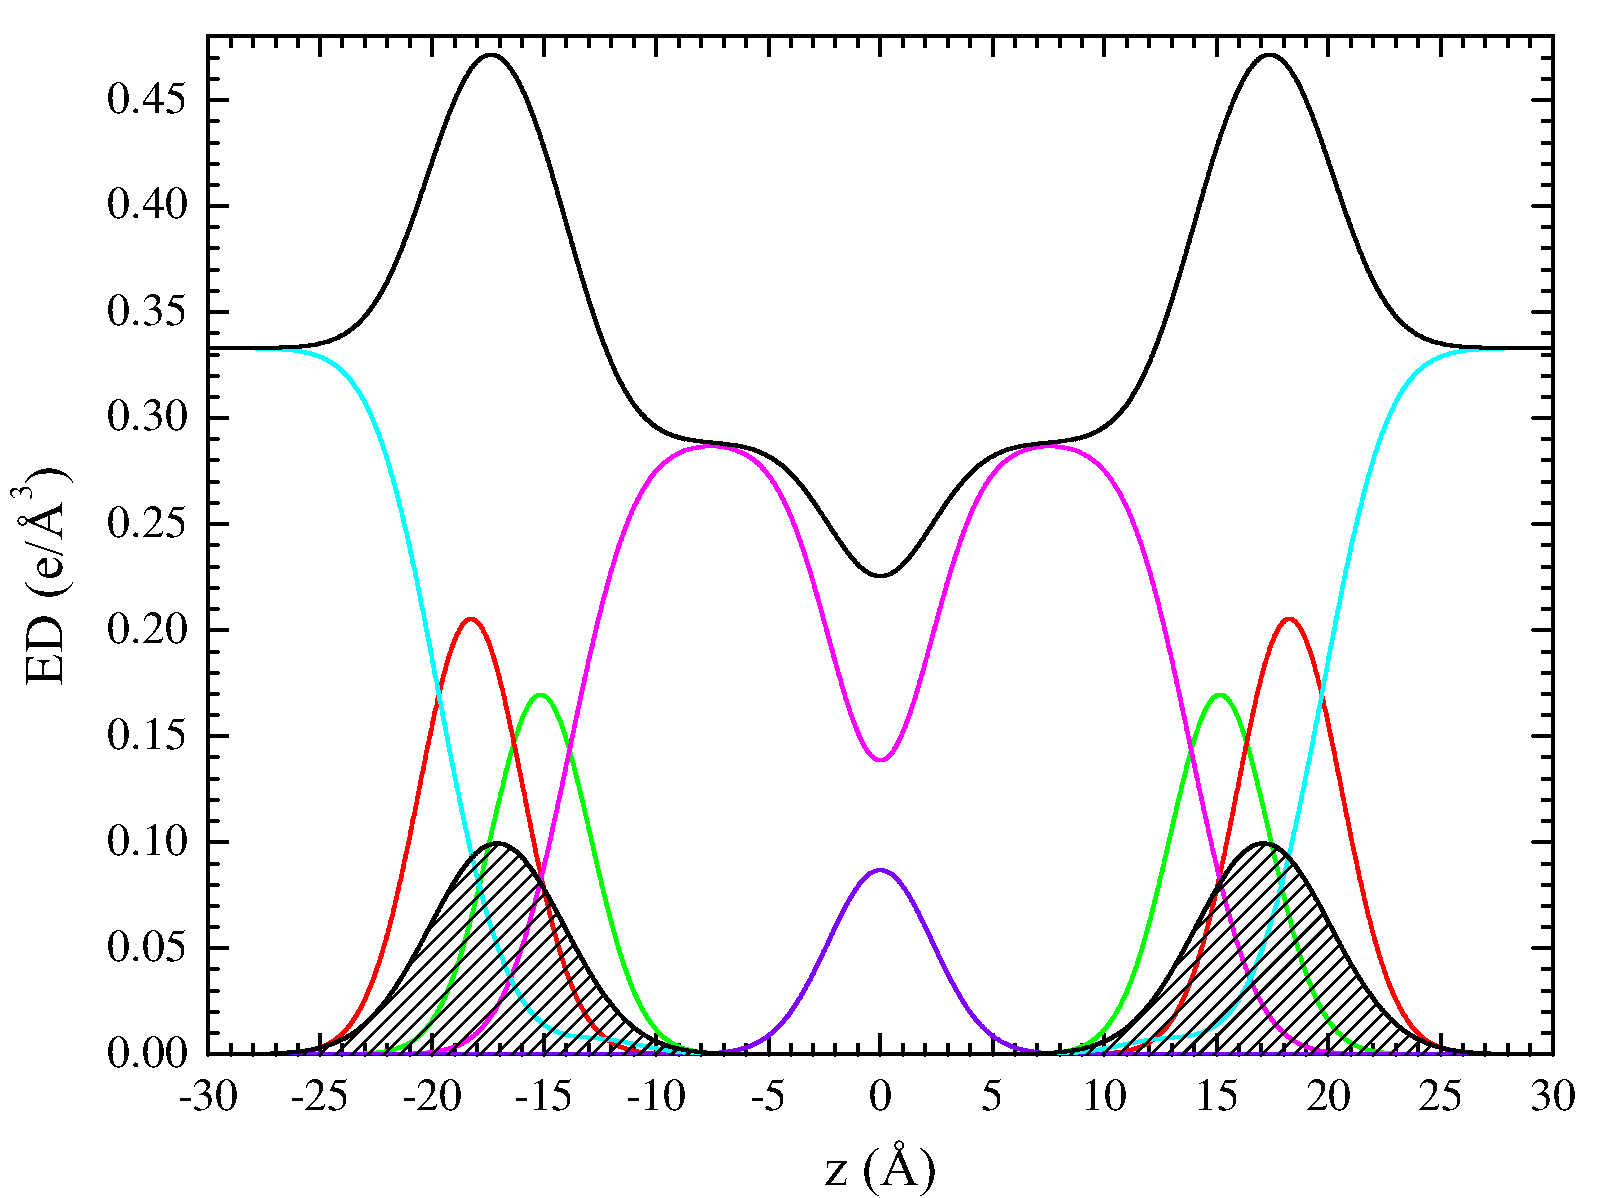
\includegraphics[width=0.45\textwidth,valign=t]{./figures/Tat/SDP_Results/EDP/DOPCDOPE1to1_Tat_16to1_3p0_EDP1}
  \caption{The best fits to DOPC:DOPE (1:1) form factors (left) and the corresponding 
  electron density profiles (right) with $\xTat$ = 0, 0.016, 0.034, 
  and 0.059 (from top to bottom).}
  \label{fig:DOPCDOPE1to1_Tat_XFF1}
\end{figure}
%------------------------------------------------------------------------------
\begin{table}[htbp]
  \centering
  \begin{tabular}{|c|c|c|c|c|c|c|c|c|c|c|}
    \hline
    $\xTat$ & 0 & \multicolumn{3}{c|}{1/63} & \multicolumn{3}{c|}{1/29} & \multicolumn{3}{c|}{1/17} \\
    \hline
    $\chi^2$ & 2961 & 1554 & 1570 & 1581 & 1563 & 1587 & 1607 & 2342 & 2338 & 2363 \\ 
    $\chi^2_\textrm{red}$ & 5.307 & 2.785 & 2.813 & 2.833 & 2.807 & 2.849 & 2.885 & 4.197 & 4.189 & 4.235 \\
    \hline
    $\zPC$ & 18.1 & 18.0 & 17.9 & 17.9 & 17.8 & 17.7 & 17.6 & 17.8 & 17.8 & 17.7 \\
    $\sigmaPC$ & 2.52 & 2.14 & 2.17 & 2.18 & 1.86 & 1.92 & 1.93 & 2.02 & 1.97 & 1.93 \\
    $\zCG$ & 15.0 & 14.9 & 14.8 & 14.8 & 14.7 & 14.6 & 14.5 & 14.7 & 14.7 & 14.6 \\
    $\sigmaCG$ & 3.00 & 2.62 & 2.64 & 2.66 & 2.22 & 2.30 & 2.31 & 2.58 & 2.27 & 2.14 \\
    $\zHC$ & 13.7 & 13.6 & 13.5 & 13.5 & 13.4 & 13.3 & 13.2 & 13.4 & 13.4 & 13.3 \\ 
    $\sigmaHC$ & 3.00 & 2.69 & 2.84 & 2.95 & 2.65 & 2.82 & 3.01 & 2.47 & 2.58 & 2.83 \\
    $\sigmaCHthree$ & 3.20 & 3.19 & 3.22 & 3.24 & 3.37 & 3.43 & 3.47 & 2.70 & 2.70 & 2.74 \\
    $\zTat$ & NA & 12.9 & 13.4 & 14.2 & 13.1 & 13.8 & 14.4 & 15.2 & 15.2 & 15.7 \\
    $\sigmaTat$ & NA & 2.5 & 3.0 & 3.5 & 2.5 & 3.0 & 3.5 & 2.5 & 3.0 & 3.5 \\ 
    \hline
    $\VL$ & 1314 & \multicolumn{3}{c|}{1344} & \multicolumn{3}{c|}{1380} & \multicolumn{3}{c|}{1432} \\ 
    $\VHL$ & 331 & \multicolumn{3}{c|}{362} & \multicolumn{3}{c|}{397} & \multicolumn{3}{c|}{450} \\
    $\VTat$ & 0 & \multicolumn{3}{c|}{30.5} & \multicolumn{3}{c|}{66.1} & \multicolumn{3}{c|}{118.8} \\
    $\RPC$ & 0.59 & \multicolumn{3}{c|}{0.54} & \multicolumn{3}{c|}{0.49} & \multicolumn{3}{c|}{0.43} \\
    $\RCG$ & 0.41 & \multicolumn{3}{c|}{0.38} & \multicolumn{3}{c|}{0.0.34} & \multicolumn{3}{c|}{0.30} \\
    \hline
    $\Delta z_1$ & \multicolumn{10}{c|}{3.1} \\
    $\Delta z_2$ & \multicolumn{10}{c|}{1.3} \\
    $\rCHthree$ & \multicolumn{10}{c|}{1.97} \\
    $\rTat$ & \multicolumn{10}{c|}{0} \\
    \hline
    $\AL$ & 71.5 & 72.4 & 72.5 & 72.7 & 73.6 & 74.0 & 74.4 & 73.6 & 73.5 & 73.9 \\
    \hline
  \end{tabular}
  \caption{Fitting Results for DOPC:DOPE (1:1) membranes. $\Delta z_1 = \zPC-\zCG$
  and $\Delta z_2 = \zCG-\zHC$. (Need to work)}
  \label{tb:DOPCDOPE1to1_fit_results}
\end{table}
%------------------------------------------------------------------------------

We also investigated how the goodness of fits varied as the placement of 
the Tat Gaussian was varied. Figure~\ref{fig:DOPC_Tat_X2} plots $\chi^2$ as a 
function of fixed Tat position, $\zTat$. We found that model A and B resulted 
in similar electron density profiles, yielding similar $\chi^2$ values 
when Tat was placed near the hydrocarbon-water interface region. In model B, 
the error function representing the hydrocarbon chain region became wider as the 
Tat component was placed deeper into the headgroup region. The subtraction
of the Tat component from the hydrocarbon chain error function resulted in 
a smooth error function-like profile with a smaller value of $\sigma$ such that
the total profile calculated from model B was very similar to that calculated 
from model A.
%------------------------------------------------------------------------------
\begin{figure}[htbp]
  \centering
  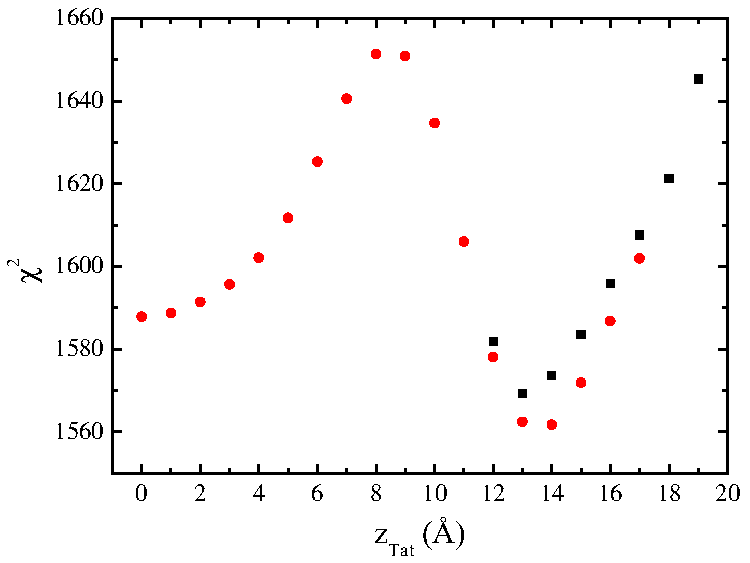
\includegraphics[width=0.3\textwidth]{figures/Tat/SDP_Results/X2/DOPC_Tat_62to1_3p0_X2} 
  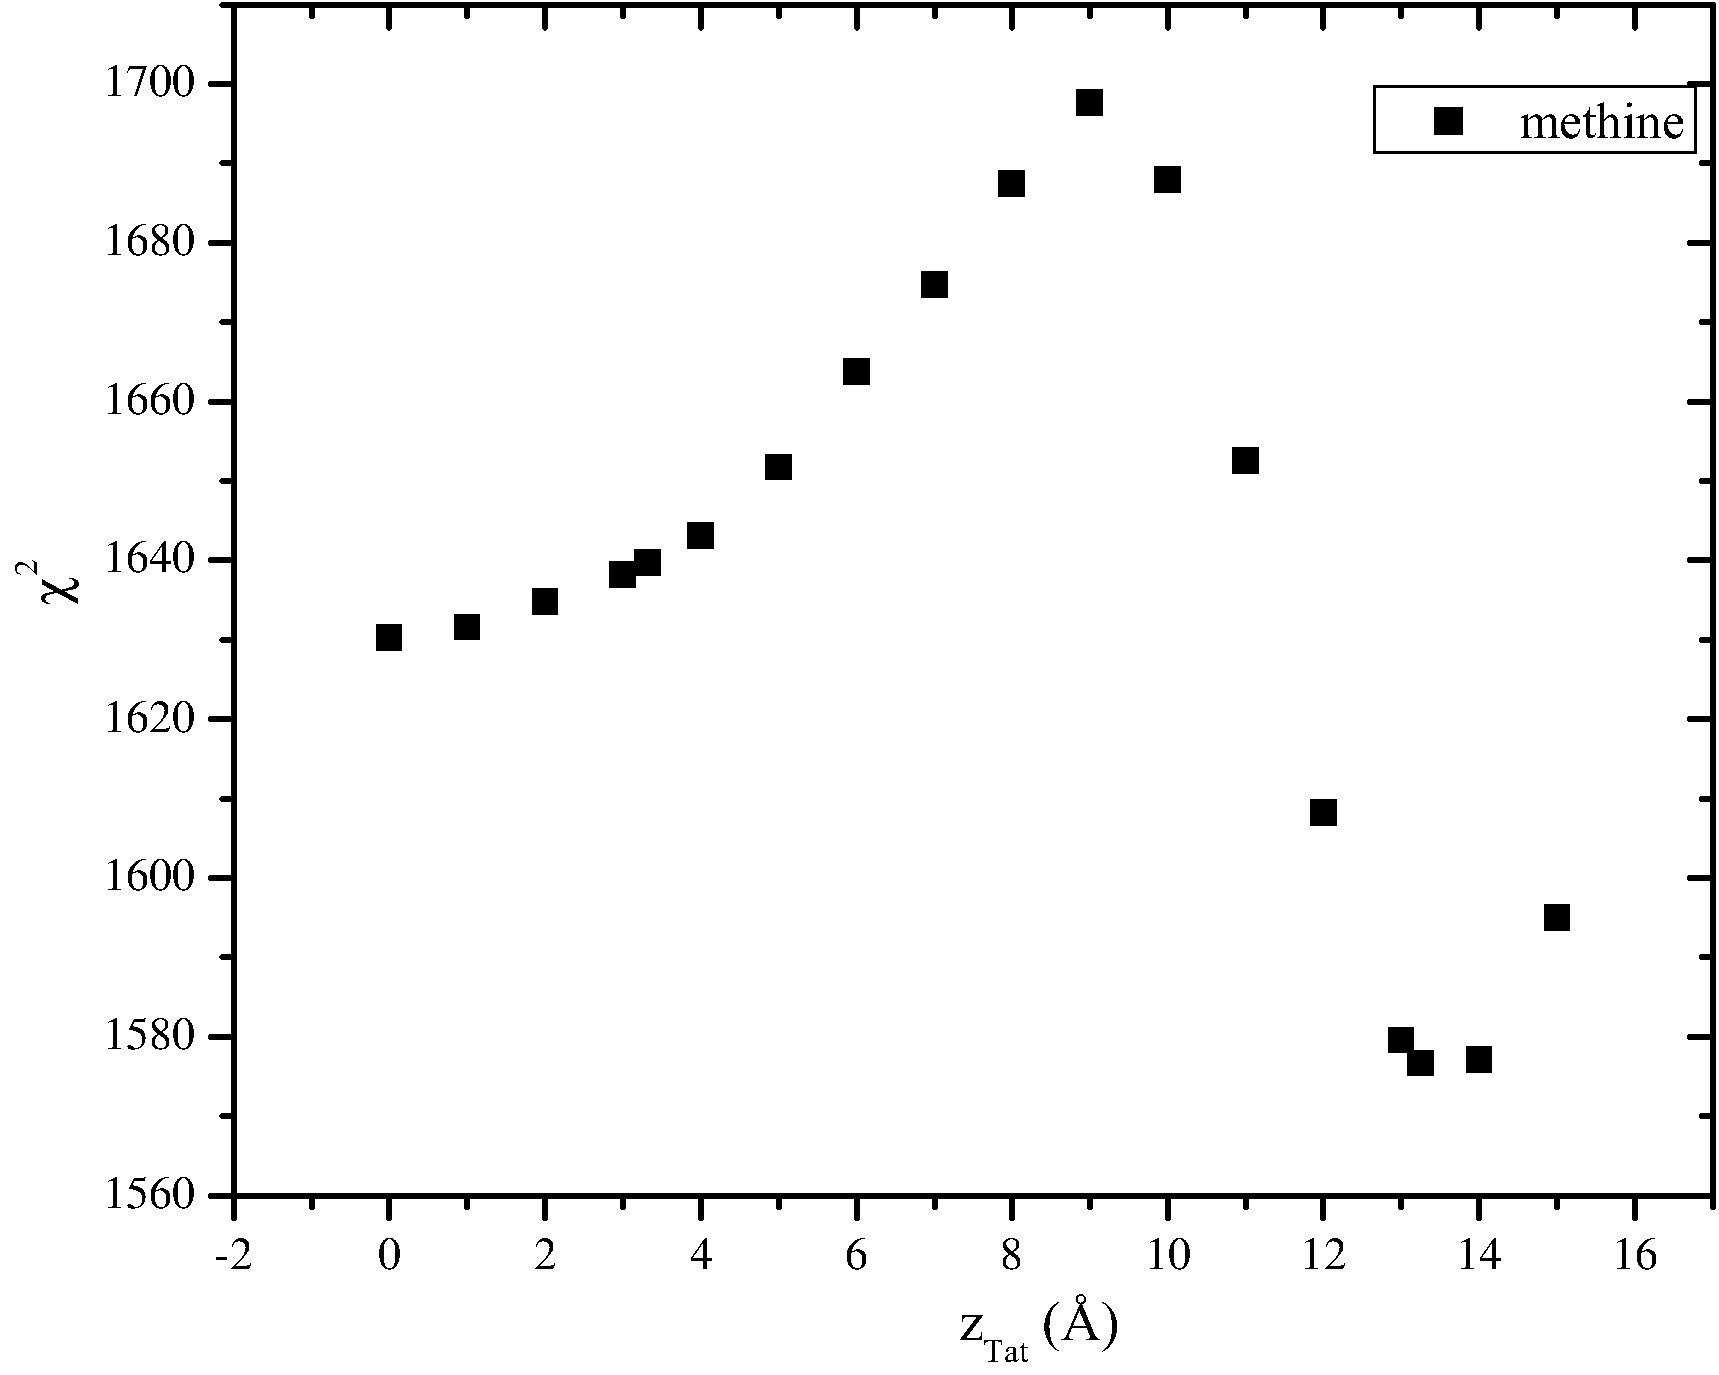
\includegraphics[width=0.3\textwidth]{figures/Tat/SDP_Results/X2/DOPC_Tat_28to1_3p0_X2} 
  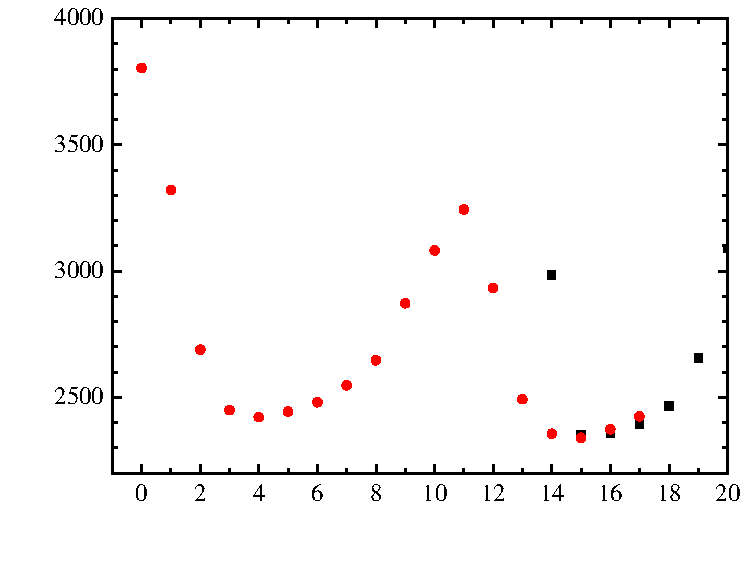
\includegraphics[width=0.3\textwidth]{figures/Tat/SDP_Results/X2/DOPC_Tat_16to1_3p0_X2}
  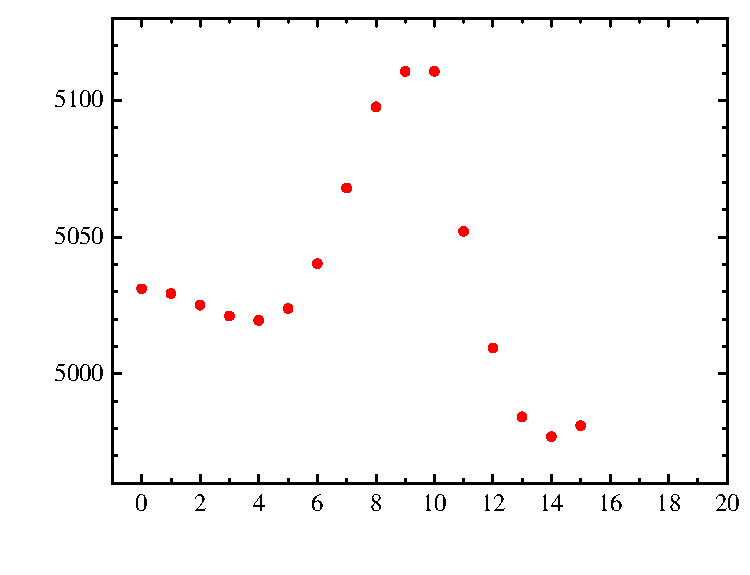
\includegraphics[width=0.3\textwidth]{figures/Tat/SDP_Results/X2/DOPCDOPE3to1_Tat_62to1_3p0_X2}
  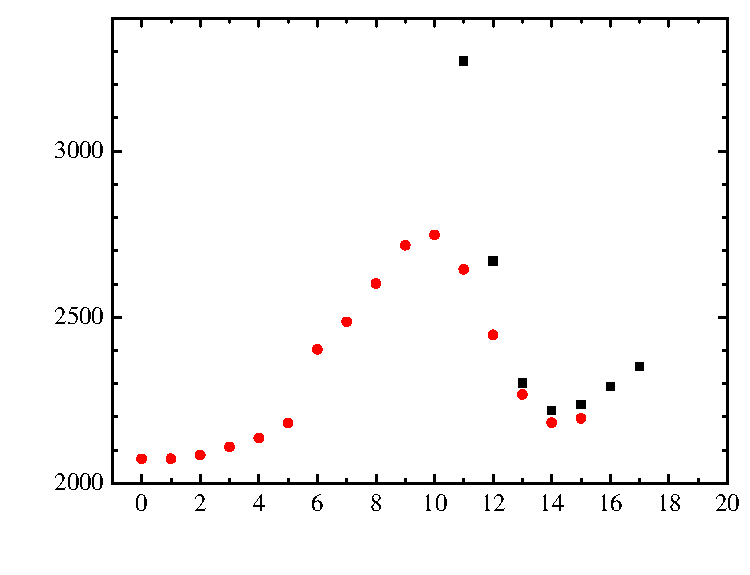
\includegraphics[width=0.3\textwidth]{figures/Tat/SDP_Results/X2/DOPCDOPE3to1_Tat_28to1_3p0_X2}
  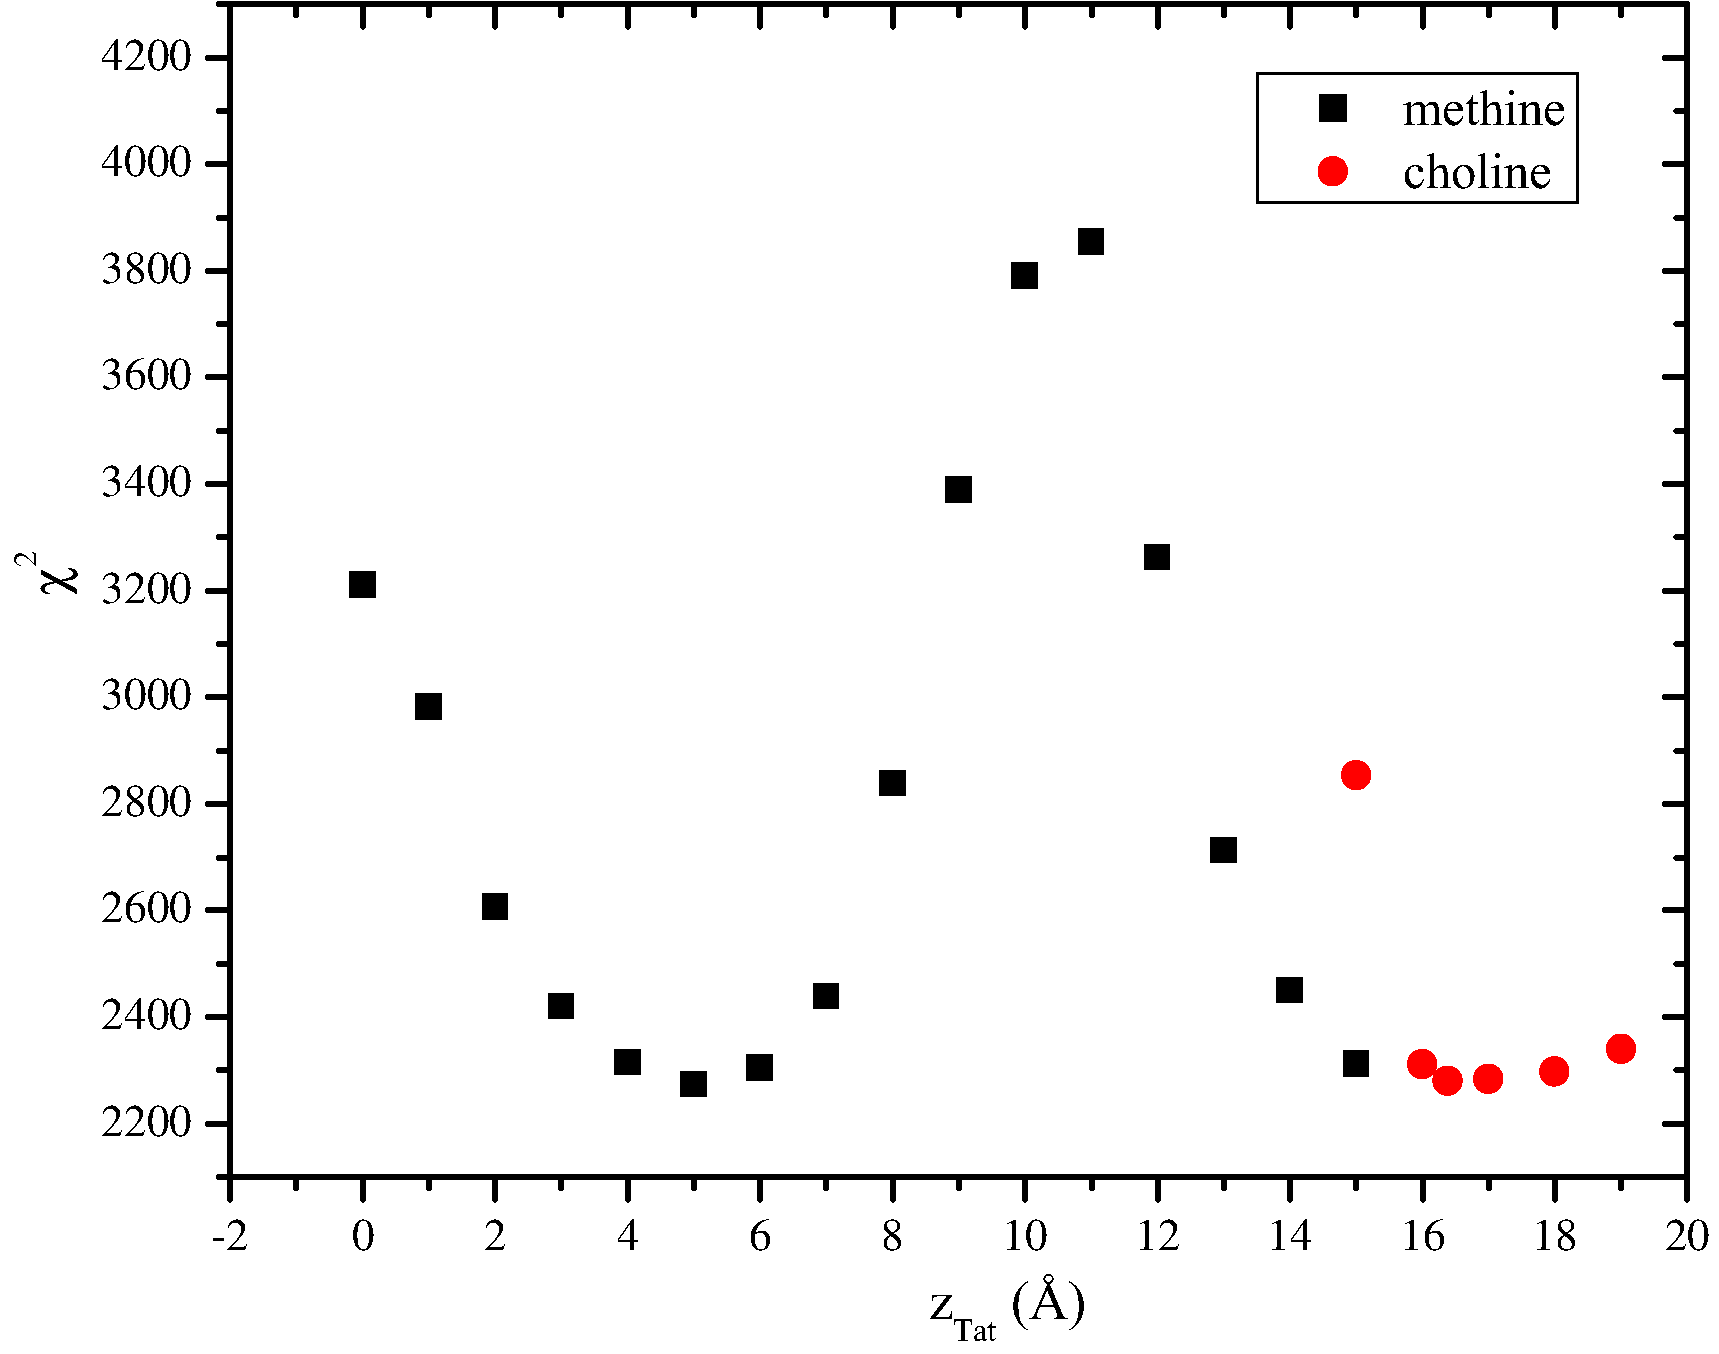
\includegraphics[width=0.3\textwidth]{figures/Tat/SDP_Results/X2/DOPCDOPE3to1_Tat_16to1_3p0_X2}
  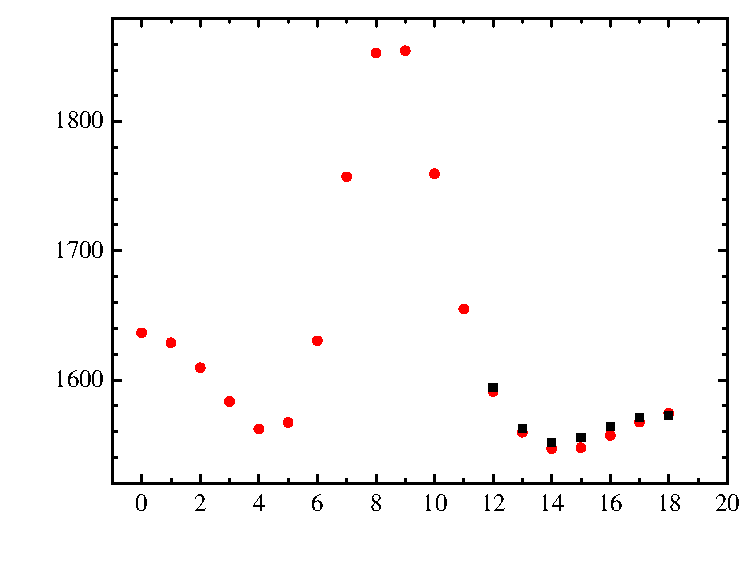
\includegraphics[width=0.3\textwidth]{figures/Tat/SDP_Results/X2/DOPCDOPE1to1_Tat_62to1_3p0_X2}
  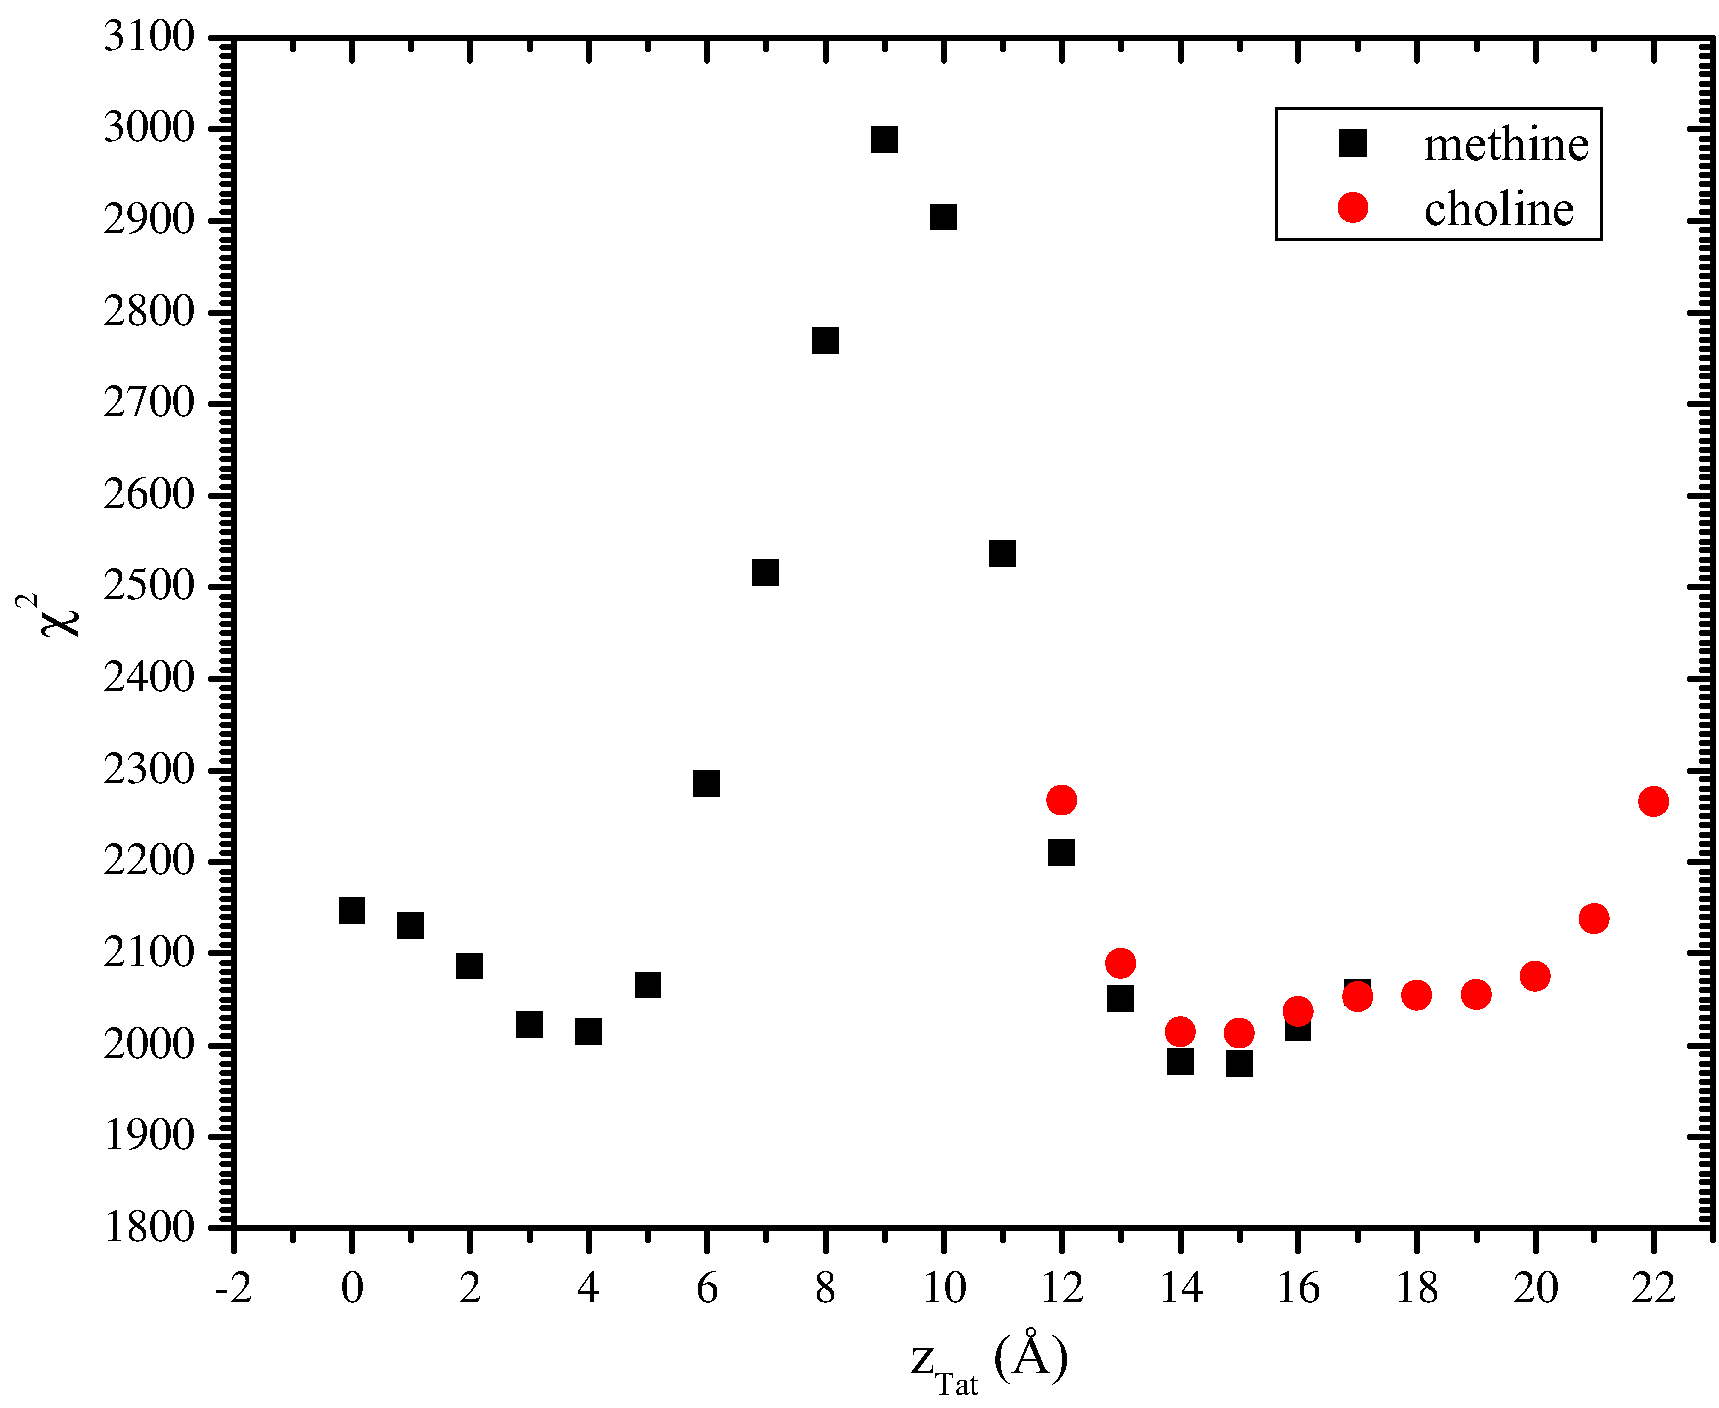
\includegraphics[width=0.3\textwidth]{figures/Tat/SDP_Results/X2/DOPCDOPE1to1_Tat_28to1_3p0_X2}
  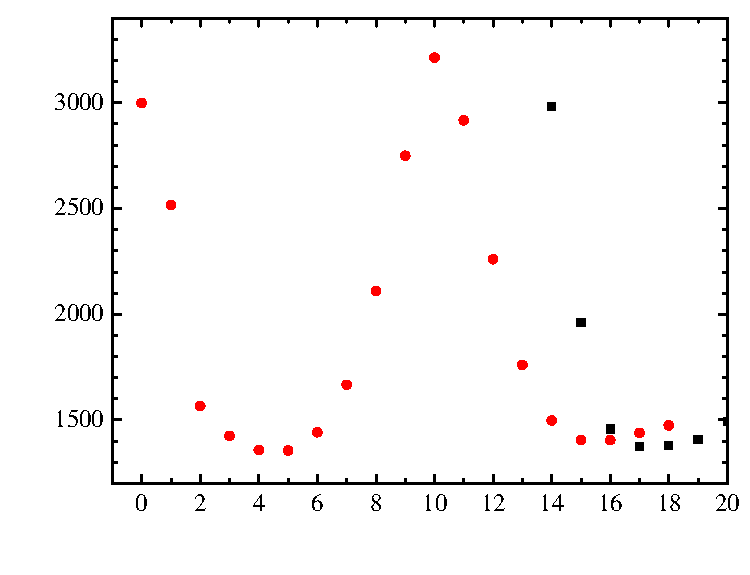
\includegraphics[width=0.3\textwidth]{figures/Tat/SDP_Results/X2/DOPCDOPE1to1_Tat_16to1_3p0_X2}
  \caption{$\chi^2$ as a function of $\zTat$ for DOPC, DOPC:DOPE (3:1), and 
  DOPC:DOPE (1:1) (from left to right) 
  with $\xTat$ = 0.016, 0.034, and 0.059 (from top to bottom).}
  \label{fig:DOPC_Tat_X2}
\end{figure}
%------------------------------------------------------------------------------

In generaly, while the total electron density profile is well determined by 
our modeling procedures, the values of the parameters for the components are 
not as well determined as the agreement of the fit to the data may suggest. 
in many cases, we found multiple local minima in the fitting landscape, 
including one with Tat closer to the center of the bilayer as
shown in Fig.~\ref{fig:DOPC_Tat_X2}. $\chi^2$ calculated at these local minima 
tended to be smaller for larger concentration of Tat. We also found
that $\chi^2$ with $\zTat$ in the hydrocarbon chain region and headgroup
region was almost equal for the smallest value of $\xTat$ for DOPC:DOPE (1:1)
bilayer.
While Fig.~\ref{fig:DOPC_Tat_X2} shows trends for the $\chi^2$ minima with Tat 
in the hydrocarbon chain region, this position seemed energetically 
unfavorable as Tat is a hydrophilic molecule. Also, if Tat favored to be 
inserted deep in a membrane, it would be difficult for Tat to
leave the membrane. This difficulty seems inefficient in terms of the HIV virus
infection because Tat passing through the nuclear membrane and binding
to the viral integrated DNA is crucial for proliferation of HIV infected cells as
discussed in section~\ref{sec:Tat_intro}. 
These considerations suggested that the local minima in the chain region
was artifact of our models.
With a help of MD simulations performed by Dr. Kun Huang,
we were able to discard the interior position as an artifact of our 
modeling. The simulation results are discussed in section~\ref{sec:sim_results}.

Electron density profiles for DOPC/DOPS (3:1) and the nuclear membrane 
mimic were not
successful, due to loss of diffuse scattering by Tat’s charge neutralization 
of these negatively
charged membranes as described in section \ref{sec:Kc_results}.

%%%%%%%%%%%%%%%%%%%%%%%%%%%%%%%%%%%%%%%%%%%%%%%%%%%%%%%%%%%%%%%%%%%%%%%%%%%%%%%
\subsection{Hard Wall Constraint Fits}
As seen from Table~\ref{tb:DOPC_fit_results}, \ref{tb:DOPCDOPE3to1_fit_results},
and \ref{tb:DOPCDOPE1to1_fit_results}, the widths of the headgroup components
became smaller as Tat concentration increased in all membranes. These 
decreases seemed somewhat unreasonable; if Tat causes a bilayer 
to locally become thinner near where it is bound, 
we would expect that the headgroup components to become
wider. Therefore, we also fitted the model with hard wall constrains
on these headgroup widths. Namely, the minimum values of the widths of
the headgroup components, PC and CG, were limited to the corresponding 
values for pure bilayers without Tat. (Need to finish analysis on this)

%%%%%%%%%%%%%%%%%%%%%%%%%%%%%%%%%%%%%%%%%%%%%%%%%%%%%%%%%%%%%%%%%%%%%%%%%%%%%%%
\subsection{Summary of Electron Density Profile Modeling}
Figs. 7A and 7B show that both these 
quantities tend to
decrease with increasing Tat mole fraction (P/(L+P)), showing that Tat thins 
membranes,
increasingly so as its concentration is increased, even though both simulation 
and modeling
suggest that Tat moves further from the membrane center with increasing 
concentration as
shown in Fig. 7D. Fig. 7C shows that the area per lipid AL usually increases 
with increasing
mole fraction of Tat, similar to the findings from MD simulations (Section 3.2), 
as would be
expected. The results from the simulation data plotted in Fig. 7 were obtained 
by using a
weighted average based on chi-square of the four best fits of the simulated 
form factors with the
experimental form factors.

Figure shows that $A_L$ as defined by $(V_L-V_{HL})/D_c$ decreases as the 
amount of DOPE increases for systems without Tat. This is consistent with the
previous studies (or predictions?) and attributed to the small size of PE
head group. Because DOPE has smaller head group than DOPC, lipids in DOPC/DOPE
bilayers pack more compactly than DOPC bilayers do, leading to a smaller $A_L$.
Consequently, bilayers composed of DOPC and DOPE tend to have a higher order 
parameter than DOPC alone. (NO THEY DON'T. WHAT'S GOING ON HERE?). Similarly,
the thickness of bilayers is larger at higher PE content. 

Figure shows that Tat is located further out from the bilayer center with 
higher content of PE lipids. This is also consistent with MD simulation PMF,
which showed that arginine insertion cost more energy for PE membrane than
PC membrane, the result of which was attributed to more possible hydrogen 
bonding between PE group and arginines.

More structural detail from the modeling and from the simulations is shown in 
Fig. 7. The bilayer thickness can be described as DHH, which is the 
distance between the maxima in the electron density profile, or as DPP, which 
is the distance between the phosphocholines on the opposing monolayers. Figs. 
7A and 7B show that both these quantities decrease with increasing Tat mole 
fraction (P/(L+P)), showing that Tat thins membranes, increasingly so as its 
concentration is increased, even though both simulation and modeling suggest 
that Tat moves further from the membrane center with increasing concentration 
as shown in Fig. 7D.  Fig. 7C shows that the area per lipid AL usually increases 
with increasing mole fraction of Tat, as would be expected from consideration of 
conservation of lipid volume. Interestingly, the bilayer thickness did not 
increase for DOPC/DOPE (3:1) bilayers with x less than 0.03.  

%%%%%%%%%%%%%%%%%%%%%%%%%%%%%%%%%%%%%%%%%%%%%%%%%%%%%%%%%%%%%%%%%%%%%%%%%%%%%%%
\subsection{Molecular Dynamics Simulations}\label{sec:sim_results}
Due to the slow relaxation in lipid bilayers and limited accuracy of the force 
field, a good
agreement between experimental and MD simulation calculated form factors may 
be difficult to
reach. Consequently, we carried out several constrained simulations at $A_L$ 
and $Z_{Tat}$ as described
in Materials and Methods. We then compared the simulated form factor $F(q_z)$ 
with the
experiment. The best match for DOPC/Tat (128:4) was found when the Tats were 
constrained at 18 \AA away from the bilayer center (Fig. 4.A,B). The other 
best fit results were: DOPC $A_L$ = 70 \AA$^2$ and DOPC/Tat(128:2) $A_L$ = 72 
\AA$^2$, $Z_{Tat} = 18$ \AA. It clearly indicates that with increasing Tat
concentration, $A_L$ increases. The agreement worsened as Tat was constrained 
to be closer to the
center of the bilayer. When Tats were constrained at 5 \AA away from the bilayer 
center, we
observed a spontaneous formation of water pores in the MD simulation. However, 
as shown in
Fig. 4.C the corresponding form factor calculated from MD simulations does not 
match well
with experiments.
Figure 4. MD simulated form factors (red solid lines in A and C) of Tat/(DOPC+Tat), x=0.030,
with Tat fixed at ZTat= 18 Å (panel A) and 5 Å (panel C) from the bilayer center compared to
experimental form factors (open circles) scaled vertically to provide the best fit to the
simulations. Corresponding snapshots are shown in Panels B and D in which the lipid chains are
represented as grey sticks on a white background, Tats are yellow, phosphate groups are red and
water is blue.



\subsection{Summary of Results}
We summarize our results for how Tat affects the lipid bilayer in Fig. 9. 
The height of Tat, $H_{Tat} = 8.7$ \AA, was the full width at half maximum of 
the Tat electron density profiles
obtained from simulations and the cylindrical radius, $R_{Tat} = 8.3$ \AA, was 
calculated to give the
measured volume. The $Z$ distances from the center of the bilayer were derived 
from weighted
averages of four MD simulations of Tat:DOPC 2:128. The $\chi^2$ obtained by 
comparison to
experiment indicated that the best $Z_{Tat}$ lay between the simulated values 
of 16 \AA and 18 \AA and
the best area/lipid $A_L$ lay between the simulated values of 72 \AA$^2$ and 
74 \AA$^2$, 
so averages were
obtained from these four combinations of $Z_{Tat}$ and $A_L$, weighted inversely 
with their $\chi^2$. The
average positions, Z'Phos, of phosphates situated underneath the Tats were calculated by
averaging over the phosphates whose in-plane distance, R, from the center of Tat is smaller than
RTat. The simulation cell extended to 38 \AA, far enough to ensure that ZPhos for most of the lipids is
the same as for DOPC. Assuming a simple linear ramp in ZPhos, Fig. 9 then indicates a ring of
boundary lipids that extends twice are far in R as Tat itself. Although the guanidinium electron
density profile was broad (Fig. S8), indicating that some were pointing away from the bilayer
relative to the center of Tat, more were pointing towards the bilayer center as indicated in Fig. 9.
Numerical values are given in Table S1.

\section{Discussion}
Given that 8 of the 11 amino acids in Tat (47-57) are arginines and lysines, 
one would have
suggested 20 years ago that highly charged Tat would partition strongly into 
solution rather than
being associated with lipid bilayers. By contrast, but in agreement with more 
recent perspectives
on arginine partitioning into the interfacial region [58], we find that Tat
interacts with lipid
bilayers, even with neutral DOPC and DOPC/DOPE mixtures, as well as with 
negatively
charged DOPC/DOPS and nuclear membrane mimic lipid mixtures. This paper 
presents
multiple lines of evidence for a Tat/membrane interaction. Fig. 2 shows that 
Tat decreases the
bending modulus. Although one could argue that such a decrease is only apparent 
and could
instead be due to local changes in membrane spontaneous curvature [59], either 
interpretation
supports a Tat-bilayer interaction. The changes with increasing Tat 
concentration in the X-ray
membrane form factors in Fig. 3 prove that Tat affects membrane structure, 
and the shift of the
zero positions to higher qz suggests thinning. Thinning is substantiated by 
quantitative analysis
of the X-ray data and by MD simulations. Fig. 7A shows that the average 
membrane thickness,
as measured by the distance DPP between phosphocholines on opposite surfaces, 
decreases with
increasing Tat concentration. Similar thinning is shown in Fig. 7B for the 
distance DHH between
the maxima in the electron density profiles of opposite surfaces. Compared to 
DPP, DHH is pulled
towards both the carbonyl/glycerol groups and Tat because both have electron 
densities (~0.4
e/Å3) greater than water (~0.33 e/Å3) or hydrocarbon (~0.3 e/Å3). Although 
the thinning shown
in Figs. 7A and 7B is not large, it obviously requires interaction of Tat with 
the bilayers. Fig.
7C shows that AL increases with increasing Tat concentration, by both model 
fitting and MD
simulations.

It is of considerable interest to learn where Tat resides, on average, in the 
membrane, as
this would establish a base position from which translocation would be initiated.
We have
combined our two main methods, MD simulations and X-ray scattering, to address 
this question.
In general, Tats locate at the bilayer/water interface as indicated in Section 3.2, 
and they are
close to the phosphocholine headgroup region by comparing the simulated 2ZTat
in Fig. 7.D with
7.A. Although the SDP modeling of the X-ray data obtains excellent fits to the experimental
form factors for a model with Tat deep in the hydrocarbon interior (see Fig. S5), the
corresponding MD simulation (shown in Fig. 4.C) eliminates this spurious result. Fig. 7D also
shows that modeling gives smaller values for ZTat than the simulation. The modeling result is
supportive of the original simulation result of Herce and Garcia that Tat resides closer to the
bilayer center than do the phosphocholine groups [60]. That is a base position that would be a
possibly important precursor to translocation, as would the larger AL.

Several groups have carried out calculations and MD simulations showing that the cost of
moving an arginine group from water to the bilayer center is ~12-26 kcal/mol [58, 61-63] or 6-7
kcal/mol if side-chain snorkeling to the surface is taken into account [64]. This is not inconsistent
with our result that Tat interacts with the membrane because, as is well known, the bilayer is not
just a hydrocarbon slab, but has interfacial headgroup regions where Tat can reside. It has been
suggested that the free energy cost for charged amino acids entering the headgroup region is
similar to that for partitioning into octanol, about an order of magnitude smaller free energy cost
than partitioning into cyclohexane [65-67]. Simulations suggest that the free energy is smaller
for an arginine residing in the interfacial region than in water, roughly by 3 kcal/mole, depending
upon the lipid [58, 67]. Our results therefore appear energetically reasonable.

One concern with diffraction experiments on samples consisting of adjacent bilayers in a
stack or in a multilamellar vesicle is that the samples have to be partially dried to obtain
conventional diffraction data. But then there is no pure water layer between adjacent bilayers, so
a hydrophilic peptide is forced into the interfacial, partially hydrophilic region of the lipid
bilayer. In contrast, by using diffuse scattering, we obtained structure from experimental
samples that had a range of lamellar D spacings (see Fig. 2 caption) that were considerably
larger than the thickness of the bilayer in Fig. 7A, thereby providing an ample pure water space,
typically greater than 20Å. The result that 2ZTat shown in Fig. 7D is so much smaller than our
repeat spacings shows that Tat preferentially associates with the membrane rather than
dissociating into water.

Consistent with Tat softening the bilayers (Fig. 2), it also disorders them as indicated by
Sxray decreasing with Tat concentration shown in Fig. 8. Tat also increases the mosaic spread
observed by X-ray and neutron scattering as shown in Figs. S1-3; this is a much larger scale
disordering of the stack of bilayers. As shown in Table 1 and in Fig. S7, Tat assumed slightly
>50% β structures, both when dissolved in water and in contact with a hydrated thin film
membrane. Our results were determined using the DichroWEB program, which compares the
mean residue ellipticity with that from standard globular proteins, with details given in
Supplementary data near Fig. S7. These structures include approximately equal amounts of
regular β strands and turns, with ~half that amount of distorted β strands. The next most
prevalent structure was random coil (~37%). Measurements in the literature (see Section 1.
Introduction) report a primarily random structure, determined using either CD or NMR. This
difference could be due to different sample preparations, or due to a different interpretation of
the CD spectra. Ref. [68] reported that CD spectra of unordered polypeptides are similar to that
of the poly(Pro)II helix, and a significant fraction of the unordered conformation in globular
proteins consists of poly(Pro)II helix plus distorted β strands.

In an effort to better determine the secondary structure of Tat, our collaborator, Dr.
Rieko Ishima, performed 1D and 2D-NMR of Tat in solution at 10, 20 and 30oC. Her results
showed no evidence for backbone hydrogen bond formation, indicating that the peptide does not
have a stable β conformation, at least on the time scale of the NMR measurement. Additionally,
we analyzed the secondary structures of Tats from MD simulations using the Define Secondary
Structure of Proteins (DSSP) program [69]. Data from the MD simulation which has the best fit
to experimental X-ray form factors show that Tat contains neither β nor α-helix structures.
Therefore, both our solution NMR and MD simulation results find primarily random coil, with
no significant β structure, which contrasts with our CD findings of >50% β conformation. While
the interpretation of CD spectra as β, P2 helix or coil is controversial, what is clear is that the
membrane does not influence the conformation of solubilized Tat. In addition, no studies
including our own, have implicated Tat forming an α-helix, either in solution or in the
membrane.

Given our structural and elastic moduli results, we now compare to other 
experiments in
the literature. In 2008, the Wong group implicated Tat’s ability to induce saddle-splay curvature
with a potential role of bidentate hydrogen bonding as key [70]. Rhodamine-tagged Tat only
entered GUVs when the PE headgroup was included with PS and PC lipids (PS/PC/PE,
20:40:40), indicating that hydrogen-bonding, and/or curvature-promoting lipids are required for
Tat translocation. In PS/PE (20:80) lipids, they found Tat caused a highly curved cubic phase
using X-ray diffraction [70]. In our experiments, there was little effect of adding DOPE to
DOPC at either a 3:1 or 1:1 mole ratio on decrease in the bending modulus, bilayer thinning,
Tat’s outward movement with increasing concentration or disordering of chains (Sxray). Our two
results are not inconsistent, however, since curvature-promotion appears not to be required for
Tat’s ability to lower the energy required to bend, nor to locate Tat in the bilayer, nor to disorder
chains, all of which may be important for Tat translocation. Yet Tat does translocate across
membranes in their experiments only with PE in the membrane, so the ability to induce saddle-
splay curvature may also be required for Tat’s translocation. Another study by Melikov et al.
[26] found that Tat’s main mechanism of action is to induce lipid mixing and membrane leakage
with lipids of late endosomes. This result is consistent with our results that Tat induced a
reversible, hydration-induced increase in mosaic spread (Figs. S1-3) and a disordering of chains
(Fig. 8). Both of these could induce lipid mixing and perhaps, membrane leakage. An X-ray,
neutron and AFM study reported thickening upon initial Tat binding, in contradiction to our
result in Fig. 7B that shows thinning [71]. We suggest that this difference was caused by their
using stiff gel phase DPPC lipid that did not allow bound Tat to perturb the bilayer. Using a
variety of techniques, including high sensitivity isothermal titration calorimetry and 2H- and 31P-
NMR, Seelig et al. [72] presented evidence that the lipid bilayer remains intact upon Tat binding
and our results confirm this. Finally, we compare our structural results to those obtained by solid
state NMR, although at a lower hydration level than in our sample. Hong et al. [32] found that
Tat lies parallel to the bilayer surface in the headgroup region of DMPC/DMPG (8:7) bilayers,
similar to our cartoon in Fig. 9.

\section{Conclusion}
Although a recent MD simulation using umbrella sampling [73] found that the 
free
energy required for cR9 to traverse a membrane was smaller if a water pore was 
present, we
cannot directly test the existence of a transient water pore from our X-ray or 
neutron scattering
experiments. This is because, even with a water pore, the translocation process 
still requires
crossing a free energy barrier which is a non-equilibrium process. X-ray form 
factors measure
an equilibrium state. If the form factors obtained from water pore structures 
agreed well with
experiments, it would indicate that the pore structure was thermodynamically 
stable. This may
be the case for some antimicrobial peptides, but certainly not for 
cell-penetrating peptides.
Finding a kinetically competent pathway for the interesting phenomenon of 
translocation
of highly charged Tat through hydrophobic membranes is difficult. An 
energetically passive
translocation likely occurs very seldom on an MD simulation time scale, and 
it probably happens
quickly, so it would not significantly change the average structure of the 
membrane in which it
occurs. Although our results in this paper do not reveal a kinetically competent 
pathway, they do
show that Tat is drawn to the surface of the membrane, and is therefore ready 
for translocation at
a region of local thinning. And they show that these interactions tend to 
soften (Fig. 2) and
disorder (Fig. 8) the membrane and increase the AL, thereby likely reducing 
the energy barrier
for passive translocation.

